% This is the Reed College LaTeX thesis template. Most of the work
% for the document class was done by Sam Noble (SN), as well as this
% template. Later comments etc. by Ben Salzberg (BTS). Additional
% restructuring and APA support by Jess Youngberg (JY).
% Your comments and suggestions are more than welcome; please email
% them to cus@reed.edu
%
% See http://web.reed.edu/cis/help/latex.html for help. There are a
% great bunch of help pages there, with notes on
% getting started, bibtex, etc. Go there and read it if you're not
% already familiar with LaTeX.
%
% Any line that starts with a percent symbol is a comment.
% They won't show up in the document, and are useful for notes
% to yourself and explaining commands.
% Commenting also removes a line from the document;
% very handy for troubleshooting problems. -BTS

% As far as I know, this follows the requirements laid out in
% the 2002-2003 Senior Handbook. Ask a librarian to check the
% document before binding. -SN

%%
%% Preamble
%%
% \documentclass{<something>} must begin each LaTeX document
\documentclass[12pt,oneside]{reedthesis}
% Packages are extensions to the basic LaTeX functions. Whatever you
% want to typeset, there is probably a package out there for it.
% Chemistry (chemtex), screenplays, you name it.
% Check out CTAN to see: http://www.ctan.org/
%%

\usepackage[normalem]{ulem}
\usepackage[spanish,es-tabla]{babel}
\usepackage{setspace}\onehalfspacing%%%\doublespacing
\usepackage{float}

\usepackage{graphicx,latexsym}
\usepackage{amsmath}
\usepackage{amssymb,amsthm}
\usepackage{longtable,booktabs,setspace}
\usepackage{chemarr} %% Useful for one reaction arrow, useless if you're not a chem major
\usepackage[hyphens]{url}
% Added by CII
\usepackage{hyperref}
\usepackage{lmodern}
\usepackage{float}
\floatplacement{figure}{H}
% End of CII addition
\usepackage{rotating}

% Next line commented out by CII
%%% \usepackage{natbib}
% Comment out the natbib line above and uncomment the following two lines to use the new
% biblatex-chicago style, for Chicago A. Also make some changes at the end where the
% bibliography is included.
%\usepackage{biblatex-chicago}
%\bibliography{thesis}


% Added by CII (Thanks, Hadley!)
% Use ref for internal links
\renewcommand{\hyperref}[2][???]{\autoref{#1}}
\def\chapterautorefname{Capítulo}
\def\sectionautorefname{Sección}
\def\subsectionautorefname{Subsección}
% End of CII addition

% Added by CII
\usepackage{caption}
\captionsetup{width=5in}
% End of CII addition

% \usepackage{times} % other fonts are available like times, bookman, charter, palatino

% Syntax highlighting #22

% To pass between YAML and LaTeX the dollar signs are added by CII
\title{Curva de Beveridge}
\author{Federico Molina Magne}
% The month and year that you submit your FINAL draft TO THE LIBRARY (May or December)
\date{28 de febrero de 2020}
\division{Facultad de Ciencias Económicas y de Administración}
\advisor{Rodrigo Ceni}
\institution{Universidad de la República}
\degree{Magíster en Economía}
%If you have two advisors for some reason, you can use the following
% Uncommented out by CII
% End of CII addition

%%% Remember to use the correct department!
\department{Economía}
% if you're writing a thesis in an interdisciplinary major,
% uncomment the line below and change the text as appropriate.
% check the Senior Handbook if unsure.
%\thedivisionof{The Established Interdisciplinary Committee for}
% if you want the approval page to say "Approved for the Committee",
% uncomment the next line
%\approvedforthe{Committee}

% Added by CII
%%% Copied from knitr
%% maxwidth is the original width if it's less than linewidth
%% otherwise use linewidth (to make sure the graphics do not exceed the margin)
\makeatletter
\def\maxwidth{ %
  \ifdim\Gin@nat@width>\linewidth
    \linewidth
  \else
    \Gin@nat@width
  \fi
}
\makeatother

\renewcommand{\contentsname}{Índice general}
% End of CII addition

\setlength{\parskip}{0pt}

% Added by CII

\providecommand{\tightlist}{%
  \setlength{\itemsep}{0pt}\setlength{\parskip}{0pt}}

\Acknowledgements{
Quiero agradecer a toda mi familia y amigos, a mi tía Maritza, Norberto y primas que no veo hace más de diez años. Mi abuela lulo y tíos Jorge y Paola que no van a poder estar y me vieron crecer, a mi grandes amigos casi hermanos Pancho (y sus viejos), el gordo droga, wismael, paoli, motuco, manolete (y al comandante), a la banda supercheto y otros tantos que tampoco van a poder estar. A mis amigos de acá (pero que están de viaje y tampoco van a poder estar! Ya tomaremos una y discutiremos de economía, política y series temporales!) rafa, joaco, claudio y eri. Germán y Augusto (ustedes si tienen que ir! Después vamos a tomar una..) y manuel y antonio con quienes discutimos y bebemos café. A mi tutor, Rodrigo que me banco y relajo merecidamente cuando me rasque las bolas (lo compadezco! No fui el mejor tesista). También a Natalia con quien trabaje el último año en el IESTA y me sirvió un montón, ya soy un R boy (y este año volvemos a trabajar!) y a Silvia de quién fui ayudante el año pasado y este año ya soy ayudante oficial!
Por último y con especial enfásis quiero agradecer a papa, la abuela Mirna, Vane mi novia :) , mama y mi hermana. Porque en cada momento que me ha tocado estar con ustedes me han ayudado de forma permanente, en las buenas y en las malas.
A todos muchas gracias, me hubiese gustado dedicarles un mejor trabajo pero bueno\ldots{}Será para el doctorado! (sera?)
}

\Resumen{

}

\Dedication{
Dedico este trabajo a mi abuelo quien acaba de fallecer y me dejo muchas enseñanzas, de las cuales quiero destacar dos. La primera es que no importa la circunstancia, siempre se debe actuar de forma correcta y ser honesto. La segunda es que fue quien me inculco que estudiar es la única forma de superarse y salir adelante, como siempre me decía (y yo no hacía caso porque era un vago\ldots{} ahora no tanto) ``¿Qué es lo que tiene que hacer un estudiante? Estudiar, estudiar y estudiar!''. A mi abuelo, a quien no pude ver por la distancia que nos separaba, le mando un abrazo.
}

\Preface{

}

\Abstract{
\par

La curva de Beveridge (CB) se plantea como una relación negativa entre la tasa de vacantes laborales y la tasa de desempleo. Las vacantes se entienden como aquella posición dentro de la firma que el empleador busca llenar activamente en un periodo a determinar. Es utilizada como un proxy de la demanda laboral cuantificándose mediante los avisos laborales publicados en la prensa o portales de Internet. Los desocupados se definen como personas buscando trabajo remunerado activamente que no logran obtenerlo durante un periodo de referencia. La CB es el marco teórico dominante en el análisis macroeconómico del mercado laboral puesto que contiene información esencial para analizar los shocks, la coexistencia de vacantes y desempleo, el proceso de matching y la eficiencia.

\par

Pese a su relevancia no es posible calcular la CB en Uruguay porque no se cuenta con información de vacantes laborales. Por ello, el primer objetivo específico de este trabajo es sistematizar datos existentes respecto a vacantes laborales cuya metodología permita una armonización de las series de vacantes. Extender el periodo de análisis en base a información recabada a partir del diario El País, clasificados laborales, \emph{Gallito Luis} y los portales laborales \emph{Buscojobs} y \emph{Computrabajo} mediante scraping web y conteo de avisos en prensa laboral, imputación de datos faltantes y análisis de texto. Creando un índice de vacantes laborales de frecuencia trimestral de carácter público y prolongado que se convierta en una herramienta de análisis macroeconómico. El mismo siempre es condicional al departamento de Montevideo.

\par

Posteriormente se busca responder si existe algún cambio de pendiente o traslado en la CB en el periodo considerado, para lo cual se utilizan dos estrategias empíricas. Se pone a prueba la hipótesis nula de que no existe un cambio estructural en la relación de vacantes y desempleo bajo diferentes test de quiebre estructural, se plantean test de tipo dating que obtienen la cantidad de quiebres estructurales optimizando una función objetivo bajo el algoritmo de programación dinámica y se estiman las CB para los periodos obtenidos. Finalmente se plantea la estimación de la curva de Beveridge mediante vectores autorregresivos de parámetros variables y volatilidad estocástica para analizar cambios de la relación entre vacantes y desempleo, identificado bajo un modelo básico de búsqueda y emparejamiento, con restricciones de identificación de Cholesky y estimado de forma bayesiana bajo el muestreo de Gibbs.

\textbf{Clasificación ( ----- ):}
\begin{itemize}
\tightlist
\item
  \emph{Mercado laboral \textasciitilde{}\textgreater{} ---- \textasciitilde{}\textgreater{} ------}
\item
  \emph{Series temporales \textasciitilde{}\textgreater{} ---- \textasciitilde{}\textgreater{} ----}
\end{itemize}
\textbf{Palabras claves:} \emph{Curva de Beveridge - Vacantes laborales - TVP-VAR-SV - Quiebres estructurales}
}

	\usepackage[spanish]{babel}
\usepackage{footmisc}
\usepackage{amsmath}
\usepackage{subfig}
\usepackage{pdflscape}
	\usepackage{booktabs}
\usepackage{longtable}
\usepackage{array}
\usepackage{multirow}
\usepackage{wrapfig}
\usepackage{float}
\usepackage{colortbl}
\usepackage{pdflscape}
\usepackage{tabu}
\usepackage{threeparttable}
\usepackage{threeparttablex}
\usepackage[normalem]{ulem}
\usepackage{makecell}
\usepackage{xcolor}
% End of CII addition
%%
%% End Preamble
%%
%
\begin{document}

% Everything below added by CII
  \maketitle



\frontmatter % this stuff will be roman-numbered
\pagestyle{empty} % this removes page numbers from the frontmatter
  \begin{dedication}
    Dedico este trabajo a mi abuelo quien acaba de fallecer y me dejo muchas enseñanzas, de las cuales quiero destacar dos. La primera es que no importa la circunstancia, siempre se debe actuar de forma correcta y ser honesto. La segunda es que fue quien me inculco que estudiar es la única forma de superarse y salir adelante, como siempre me decía (y yo no hacía caso porque era un vago\ldots{} ahora no tanto) ``¿Qué es lo que tiene que hacer un estudiante? Estudiar, estudiar y estudiar!''. A mi abuelo, a quien no pude ver por la distancia que nos separaba, le mando un abrazo.
  \end{dedication}
  \begin{acknowledgements}
    Quiero agradecer a toda mi familia y amigos, a mi tía Maritza, Norberto y primas que no veo hace más de diez años. Mi abuela lulo y tíos Jorge y Paola que no van a poder estar y me vieron crecer, a mi grandes amigos casi hermanos Pancho (y sus viejos), el gordo droga, wismael, paoli, motuco, manolete (y al comandante), a la banda supercheto y otros tantos que tampoco van a poder estar. A mis amigos de acá (pero que están de viaje y tampoco van a poder estar! Ya tomaremos una y discutiremos de economía, política y series temporales!) rafa, joaco, claudio y eri. Germán y Augusto (ustedes si tienen que ir! Después vamos a tomar una..) y manuel y antonio con quienes discutimos y bebemos café. A mi tutor, Rodrigo que me banco y relajo merecidamente cuando me rasque las bolas (lo compadezco! No fui el mejor tesista). También a Natalia con quien trabaje el último año en el IESTA y me sirvió un montón, ya soy un R boy (y este año volvemos a trabajar!) y a Silvia de quién fui ayudante el año pasado y este año ya soy ayudante oficial!
    Por último y con especial enfásis quiero agradecer a papa, la abuela Mirna, Vane mi novia :) , mama y mi hermana. Porque en cada momento que me ha tocado estar con ustedes me han ayudado de forma permanente, en las buenas y en las malas.
    A todos muchas gracias, me hubiese gustado dedicarles un mejor trabajo pero bueno\ldots{}Será para el doctorado! (sera?)
  \end{acknowledgements}
  \begin{abstract}
    \par
    
    La curva de Beveridge (CB) se plantea como una relación negativa entre la tasa de vacantes laborales y la tasa de desempleo. Las vacantes se entienden como aquella posición dentro de la firma que el empleador busca llenar activamente en un periodo a determinar. Es utilizada como un proxy de la demanda laboral cuantificándose mediante los avisos laborales publicados en la prensa o portales de Internet. Los desocupados se definen como personas buscando trabajo remunerado activamente que no logran obtenerlo durante un periodo de referencia. La CB es el marco teórico dominante en el análisis macroeconómico del mercado laboral puesto que contiene información esencial para analizar los shocks, la coexistencia de vacantes y desempleo, el proceso de matching y la eficiencia.
    
    \par
    
    Pese a su relevancia no es posible calcular la CB en Uruguay porque no se cuenta con información de vacantes laborales. Por ello, el primer objetivo específico de este trabajo es sistematizar datos existentes respecto a vacantes laborales cuya metodología permita una armonización de las series de vacantes. Extender el periodo de análisis en base a información recabada a partir del diario El País, clasificados laborales, \emph{Gallito Luis} y los portales laborales \emph{Buscojobs} y \emph{Computrabajo} mediante scraping web y conteo de avisos en prensa laboral, imputación de datos faltantes y análisis de texto. Creando un índice de vacantes laborales de frecuencia trimestral de carácter público y prolongado que se convierta en una herramienta de análisis macroeconómico. El mismo siempre es condicional al departamento de Montevideo.
    
    \par
    
    Posteriormente se busca responder si existe algún cambio de pendiente o traslado en la CB en el periodo considerado, para lo cual se utilizan dos estrategias empíricas. Se pone a prueba la hipótesis nula de que no existe un cambio estructural en la relación de vacantes y desempleo bajo diferentes test de quiebre estructural, se plantean test de tipo dating que obtienen la cantidad de quiebres estructurales optimizando una función objetivo bajo el algoritmo de programación dinámica y se estiman las CB para los periodos obtenidos. Finalmente se plantea la estimación de la curva de Beveridge mediante vectores autorregresivos de parámetros variables y volatilidad estocástica para analizar cambios de la relación entre vacantes y desempleo, identificado bajo un modelo básico de búsqueda y emparejamiento, con restricciones de identificación de Cholesky y estimado de forma bayesiana bajo el muestreo de Gibbs.
    
    \textbf{Clasificación ( ----- ):}
    \begin{itemize}
    \tightlist
    \item
      \emph{Mercado laboral \textasciitilde{}\textgreater{} ---- \textasciitilde{}\textgreater{} ------}
    \item
      \emph{Series temporales \textasciitilde{}\textgreater{} ---- \textasciitilde{}\textgreater{} ----}
    \end{itemize}
    \textbf{Palabras claves:} \emph{Curva de Beveridge - Vacantes laborales - TVP-VAR-SV - Quiebres estructurales}
  \end{abstract}

  \hypersetup{linkcolor=black}
  \setcounter{tocdepth}{2}
  \tableofcontents

  \listoftables

  \listoffigures

\mainmatter % here the regular arabic numbering starts
\pagestyle{fancyplain} % turns page numbering back on

\hypertarget{intro}{%
\chapter{Introducción}\label{intro}}

El análisis teórico de la dinámica agregada del mercado laboral ha estado organizado en base a dos relaciones, la curva de Phillips y la curva de Beverige (Blanchard \& Diamond, \protect\hyperlink{ref-Blanchard1989}{1989}). La curva de Beveridge (en adelante CB) analizada por primera vez por Beveridge (\protect\hyperlink{ref-Beveridge}{1944}) y Dicks-Mireaux \& A. (\protect\hyperlink{ref-Dicks-Mireaux1958}{1958}) plantea una relación negativa entre la tasa de vacantes laborales y tasa de desempleo y, resume información esencial sobre el funcionamiento del mercado de trabajo y shocks que afecten al mismo (Blanchard \& Diamond, \protect\hyperlink{ref-Blanchard1989}{1989}). Las vacantes se entienden como aquella posición dentro de la firma que el empleador busca cubrir activamente durante un periodo de referencia mientras los desocupados se definen como aquellas personas que durante un periodo de tiempo buscan trabajo remunerado activamente pero no logran obtenerlo.\footnote{Ambas variables suelen ser normalizadas por la población económicamente activa (PEA), personas que pertenecer a la población en edad de trabajar (PET) y buscar hacerlo activamente.}

El objetivo principal de esta investigación es profundizar en esta relación negativa y probar si existe estabilidad parámetrica a lo largo del tiempo, por lo tanto, la pregunta de investigación busca responder si la curva de Beveridge de Uruguay entre 1980 y 2019 presenta cambios de pendientes y/o traslados paralelos en cualquier momento del periodo considerado. La hipótesis sostenida es que la relación entre vacantes y desempleo no puede ser estable para el periodo de estudio.

La medición de la tasa de trabajadores desocupados se mide regularmente a lo largo del mundo con una metodología estandarizada y validada. Mientras las vacantes son raramente calculadas bajo una metodología sistemática, no suelen ser recolectadas, ni existen encuestas al respecto a excepción de algunos países, especialmente de la OCDE (Albertini, Poirier, \& Trupkin, \protect\hyperlink{ref-ArgentinaBC2019}{2019}; Hobijn \& Şahin, \protect\hyperlink{ref-Hobijn2013}{2013}; Nickell, Nunziata, Ochel, \& Quintini, \protect\hyperlink{ref-Nickell2002}{2002}). En Uruguay no existe una serie de vacantes oficial que se publique de forma pública y sistemática.\footnote{Una explicación es que la recolección y medición de vacantes es una tarea compleja para las oficinas estadísticas encargadas de recabar dicha información, debido a la difícil definición de qué es una vacante y cuando una empresa identifica que existen vacantes y buscan llenarla (Elsby, Michaels, \& Ratner, \protect\hyperlink{ref-Elsby2015}{2015}).} Por lo tanto, el primer objetivo específico de este trabajo es crear el primer indicador de vacantes laborales reproducible, extenso y sistemático. La base de datos que se construye abarca casi 40 años, incorporando para los últimos quince años tres fuentes de datos y el análisis de datos a traves de \emph{text mining}.

Finalizado el indicador se obtiene el primer resultado empírico, el cual es una correlación positiva con el producto hasta el año 2013 y una relación negativa con la tasa de desempleo.

Para responder la pregunta se utiliza la tasa de desempleo calculada por el Instituto Nacional de Estadística (INE), la Encuesta Continua de Hogares (ECH) sistematizada por parte del Instituto de Economía (IECON), el Producto Interno Bruto (PIB) calculado por el Banco Central del Uruguay (BCU) y el indicador de vacantes laborales construido a partir de avisos de el diario El País (sección \emph{Gallito}), los portales laborales \emph{Buscojobs}, \emph{Computrabajo}, \emph{Uruguay Concursa}, el Índice Ceres de Demanda Laboral (ICDL) y los datos de vacantes provenientes de Rama (\protect\hyperlink{ref-Rama1988}{1988}) y Urrestarazu (\protect\hyperlink{ref-Urrestarazu1997}{1997}).

La hipótesis sostenida es que la relación entre vacantes y desempleo no puede ser estable para el periodo de estudio, deberíamos observar al menos uno de los siguientes efectos: cambios de pendiente, traslados de la CB y/o alteraciones en la varianza de los errores en un modelo lineal. El marco teórico utilizado para explicar la CB y fundamentar la hipótesis es el marco DMP (Pissarides, \protect\hyperlink{ref-Pissarides2000}{2000}) basado fundamentalmente en los trabajos de Pissarides (\protect\hyperlink{ref-Pissarides1985}{1985}), Mortensen \& Pissarides (\protect\hyperlink{ref-Mortensen1994}{1994}), Diamond (\protect\hyperlink{ref-Diamond1982}{1982}) quienes derivan analíticamente una CB microfundada.

Los cambios observados en la CB pueden deberse principalmente a factores institucionales (Blanchard \& Wolfers, \protect\hyperlink{ref-Blanchard2000}{2000}; Bouvet, \protect\hyperlink{ref-Bouvet2012}{2012}; Gujarati, \protect\hyperlink{ref-Gujarati1972}{1972}; Nickell et al., \protect\hyperlink{ref-Nickell2002}{2002}), factores tecnológicos (Elsby et al., \protect\hyperlink{ref-Elsby2015}{2015}; Lubik, \protect\hyperlink{ref-Lubik2013}{2013}) o a factores asociados al ciclo económico (Abraham \& Watcher, \protect\hyperlink{ref-Abraham1987}{1987}; Blanchard \& Diamond, \protect\hyperlink{ref-Blanchard1989}{1989}; Hobijn \& Şahin, \protect\hyperlink{ref-Hobijn2013}{2013}). Según el marco DMP (Pissarides, \protect\hyperlink{ref-Pissarides2000}{2000}) los movimientos sobre la curva se asocian a factores de ciclo económico mientras traslados paralelos (mayor o menor desempleo para una tasa de vacantes dada) se interpretan como cambios estructurales que afectan el \emph{matching} entre puestos y trabajadores desempleados. Los traslados pueden ser por aumentos en la tasa de destrucción de puestos laborales o modificaciones en la función de matching. Cambios en la función de matching pueden deberse a cambios en los costos de contratación, despido, seguro de desempleo y salario mínimo (Bouvet, \protect\hyperlink{ref-Bouvet2012}{2012}); existencia de derecho a huelga, ocupación y sindicalización (Nickell et al., \protect\hyperlink{ref-Nickell2002}{2002}); facilidad de la mano de obra para moverse geográficamente (Hobijn \& Şahin, \protect\hyperlink{ref-Hobijn2013}{2013}), modificaciones en las habilidades de los trabajadores y; alteraciones tecnológicas que puedan cambiar los costos de búsqueda y la probabilidad de encontrarse, osea mayor o menor eficiencia (Barnichon, Elsby, Hobijn, \& Şahin, \protect\hyperlink{ref-Barnichon2012}{2012}), como la creación de portales laborales en Internet (Elsby et al., \protect\hyperlink{ref-Elsby2015}{2015}).

Muchas de estas causas estructurales se observan en Uruguay. Por ejemplo, en la década de 1980 retorna la democracia (1985), con ella aumenta la sindicalización\footnote{El trabajo de Supervielle \& Quiñones (\protect\hyperlink{ref-Quinones2001}{2002}) muestra la caída de la cantidad de afiliados a sindicatos privados entre 1987 y 2000. No hay datos para periodos previos, sin embargo, el aumento planteado es relativo al periodo previo de dictadura en el cual la central CNT fue declarada ilegal, posteriormente el decreto 622/73 permitió la creación de sindicatos pero mediante elecciones secretas.} y se reinstauran los consejos de salarios los cuales funcionaron junto a una elevada negociación por rama de actividad del orden del 94\% (Filgueira \& Gelber, \protect\hyperlink{ref-Filgueira2003}{2003}).\footnote{Entre 1985 y 1999 la negociación por rama era de 94 \%, entre 1990-1994 de 76.4 \% y en 1995-1999 de 35 \%. La negociación por empresa entre 1985-1989 era de 6 \%, entre 1990-1994 de 21.2 \% y entre 1995-1999 de 64.4\% Filgueira \& Gelber (\protect\hyperlink{ref-Filgueira2003}{2003})} En los años 90, el efecto es inverso, disminuye la sindicalización prácticamente a la mitad (Supervielle \& Quiñones, \protect\hyperlink{ref-Quinones2001}{2002}), cae la negociación por rama de actividad a un 35\% (Filgueira \& Gelber, \protect\hyperlink{ref-Filgueira2003}{2003}) y se dejan de convocar los consejos de salarios a partir de 1992 (Antía, \protect\hyperlink{ref-Antia2001}{2001}). A partir de 2005, se promulgan un conjunto de reformas estructurales que conformando un cambio sustancial en las reglas de juego de la economía (Bergara \& Milnitsky, \protect\hyperlink{ref-Bergara2017}{2017}). Los gobiernos vuelven a convocar los consejos de salarios, fomentan la negociación por rama de actividad, establecen la protección de los trabajadores en procesos de terciarización, aumentan fuertemente el salario mínimo, limitan la jornada laboral de trabajadores rurales, regulan el trabajo del servicio doméstico y aprueban la ley de responsabilidad penal empresarial (Bergara \& Milnitsky, \protect\hyperlink{ref-Bergara2017}{2017})\footnote{Lo cual pudo generar mayor poder de negociación de los trabajadores, por ejemplo, en el aumento de la densidad sindical, ya que, la central obrera PIT-CNT cuadruplicó sus afiliados entre 2005 y 2020.}.

Además hay cambios tecnológicos relevantes en la penetración de Internet que genera el ingreso de nuevos actores en el sector de prensa laboral apareciendo los portales \emph{Buscojobs}, \emph{Computrabajo}, el funcionamiento de \emph{Gallito} a través de Internet y la creación del portal \emph{Uruguay Concursa} donde se centralizan las solicitudes de empleos públicos. Por último, la crisis 2002 genera una enorme emigración de población y desalienta a los trabajadores, lo cual repercute en una caída importante de la población económicamente activa (PEA).\footnote{Ver figura \ref{fig:PeaMontevideo} en el anexo.}

Las dos crisis económicas previamente mencionadas, sumado a una breve recesión en 1995 pueden dar explicaciones asociadas al ciclo económico. Entre 1982-1984 la crisis de la \emph{tablita} genera una caída de casi 16\% del producto, el salario real medio cae un 28\% y el desempleo en Montevideo llega al 14\% (Antía, \protect\hyperlink{ref-Antia2001}{2001}). Entre 1985-2000 el índice de horas trabajadas cae a la mitad, mientras los índices de productividad se duplican (Supervielle \& Quiñones, \protect\hyperlink{ref-Quinones2001}{2002}) y la economía tiene años de elevado crecimiento de la actividad como 1996-1998 con crecimiento de 5\% (Antía, \protect\hyperlink{ref-Antia2001}{2001}). Posteriormente, entre 1999 y el tercer trimestre de 2003 la economía entra en recesión (caída de 3.8\% y 7.7\% en la tasa de crecimiento), sufriendo una grave crisis económica y social, a nivel generalizado . Desde 2003 en adelante la economía crece de forma sistemática (entre 2004 y 2011 la tasa de crecimiento oscila entre 4.1\% y 7.8\%), hay un shock externo de commodities y un flujo importante de inversión extranjera, con lo cual hasta 2011 la tasa promedio anual de variación del IVF del PIB es 5.9\% y el desempleo se ubica en sus menores valores en cuarenta años, 5-6\%.

Dada esta multiplicidad de transformaciones en la economía uruguaya, se busca trabajar con estrategías empíricas lo suficientemente flexibles para captar posibles cambios parámetricos continuos o discretos. A modo de exploración se utilizan los test de fluctuación generalizada (Brown, Durbin, \& Evans, \protect\hyperlink{ref-Brown1975}{1975}; Kramer, Ploberger, \& Alt, \protect\hyperlink{ref-Society1988}{1988}; Kuan \& Hornik, \protect\hyperlink{ref-Kuan1995}{1995}; Ploberger, Krämer, \& Alt, \protect\hyperlink{ref-Ploberger1989}{1989}) con los cuales se encuentra evidencia de posibles quiebres estructurales tanto en media como en varianza. Se profundiza con test de quiebres estructurales de tipo F generalizados que no requieren definir el momento del cambio estructural para poner a prueba la hipótesis nula de no existencia de un cambio estructural en la relación de vacantes y desempleo (Andrews \& Ploberger, \protect\hyperlink{ref-Andrews1994}{1994}; Andrews, \protect\hyperlink{ref-Andrews1991}{1991}, \protect\hyperlink{ref-Andrews1993}{1993}; Hansen, \protect\hyperlink{ref-Hansen1992}{1992}), de esta forma se encuentra una modificación en la media del proceso en 1990, resultado obtenido previamente por Urrestarazu (\protect\hyperlink{ref-Urrestarazu1997}{1997}). Posteriormente, se utilizan test generalizados los cuales permiten obtener múltiples cambios estructurales sin imponer los momentos de dichos quiebres y, se agrega la posibilidad de un quiebre en la varianza de la relación (Bai \& Perron, \protect\hyperlink{ref-BaiPerron1998}{1998}, \protect\hyperlink{ref-BaiPerron2003}{2003}; Zeileis, Shah, \& Patnaik, \protect\hyperlink{ref-Zeileis2010}{2010}). De esta forma se obtienen cuatro CB, todas con relación negativa entre vacantes y desempleo y, con alteraciones tanto en la pendiente como en traslados paralelos, indicando un efecto importante debido a fricciones del mercado laboral.

A continuación se pleantean vectores autorregresivos con parámetros variables y volatilidad estocástica, TVP-VAR o TVP-VAR-SV (Benati \& Lubik, \protect\hyperlink{ref-Benati2013}{2013}; Lubik \& Matthes, \protect\hyperlink{ref-Lubik2016b}{2015}; Nakajima, \protect\hyperlink{ref-Nakajima2011}{2011}; Primiceri, \protect\hyperlink{ref-Primiceri2005}{2005}), identificado bajo un modelo básico de búsqueda y emparejamiento, con restricciones de identificación de Cholesky y estimado de forma bayesiana mediante el muestreo de Gibbs. Esta estrategia se elige en la medida que si bien es lineal condicional en los parámetros, el modelo completo es altamente no lineal y extremadamente flexible al permitir que los coeficientes del modelo (interceptos, rezagos, varianzas y covarianzas de errores) evolucionen como un paseo aleatorio (Lubik \& Matthes, \protect\hyperlink{ref-Lubik2016b}{2015}). De su estimación surge que tanto interceptos como rezagos no cambian a lo largo del tiempo, aunque si lo hace levemente la varianza de los errores, indicando que lo que estaría generando alteraciones en la CB son shocks de distinta indole, por ejemplo, de productividad.

Ambas estrategias concuerdan en que las varianzas de los errores se modifican a lo largo del tiempo, sin embargo llegan a conclusiones diferentes en cuanto a los interceptos y rezagos. Es un resultado común en la literatura de TVP-VAR la posibilidad de no encontrar variabilidad en intercepto y rezagos pese a que si debería existir y, si en las varianzas y covarianzas (Lubik \& Matthes, \protect\hyperlink{ref-Lubik2016b}{2015}). Los resultados indican distintas fases de la CB que pueden deberse a cambios por el ciclo económico (dadas las crisis y periodos de alto y bajo crecimiento o alteraciones de la PEA) pero también a modificaciones por shocks de productividad y mejoras tecnológicas que faciliten el \emph{match} como la creación de portales laborales web. Adicionalmente la causa puede ser de origen institucional, debido a la elevada cantidad de reformas estructurales que tuvo la economía, en especial de la década de 2000 en adelante. Por último, la enorme disminución observada en las vacantes laborales y el leve aumento del desempleo (especialmente en la comparación histórica) indican que el mercado laboral uruguayo debería haberse vuelto notoriamente más eficiente en su proceso de matching pese a reformas institucionales que deberían ir sentido opuesto (Bouvet, \protect\hyperlink{ref-Bouvet2012}{2012}; Nickell et al., \protect\hyperlink{ref-Nickell2002}{2002}). Sin embargo, para poder afirmar dicha frase es necesario agregar un análisis de flujos laborales, identificar shocks de productividad y aislar el efecto de otras variables relevantes que puedan tener influencia. Es de interés que trabajos posteriores se enfoquen en identificar las causas de los movimientos en la CB, lo cual es de suma importancia para la política económica.

La organización del documento es la siguiente:
\begin{itemize}
\item
  \textbf{\protect\hyperlink{cap:Fundamentos}{Capítulo 2}:} revisa la literatura de la curva de Beveridge en Uruguay, Estados Unidos y Europa. Expone la teoría de Búsqueda y Emparejamiento.
\item
  \textbf{\protect\hyperlink{cap:Metodologuxeda}{Capítulo 3}:} define las variables y la metodología de quiebres estructurales y TVP-VAR.
\item
  \textbf{\protect\hyperlink{cap:Datos}{Capítulo 4}:} define conceptos y fuentes de datos.
\item
  \textbf{\protect\hyperlink{cap:Resultados}{Capítulo 5}:} presenta los principales resultados, creación del índice de vacantes, estimación de la CB, test de quiebres estructurales y la estimación de un TVP-VAR
\item
  \textbf{\protect\hyperlink{cap:Discusion}{Capítulo 6}:} discute mejoras y posibles comentarios del indicador de vacantes y los resultados obtenidos de la estimación de la CB.
\item
  \textbf{\protect\hyperlink{cap:Conclusiones}{Capítulo 7}:} exhibe las conclusiones de la investigación y posibles trabajos futuros producto de la tesis, en especial posibles lineas de investigación futuras.
\end{itemize}
\hypertarget{cap:Fundamentos}{%
\chapter{Curva de Beveridge}\label{cap:Fundamentos}}

\hypertarget{revisiuxf3n-de-literatura}{%
\section{Revisión de literatura}\label{revisiuxf3n-de-literatura}}

Beveridge (\protect\hyperlink{ref-Beveridge}{1944}) es pionero en identificar las vacantes laborales como un determinante de la tasa de desempleo y, encontrar una relación negativa entre ambas variables. Dicks-Mireaux \& A. (\protect\hyperlink{ref-Dicks-Mireaux1958}{1958}) plantean por primera vez la CB gráficamente al examinar la confiabilidad del uso de vacantes y desempleo para ilustrar tendencias en la demanda de trabajo. Entienden y utilizan la CB para medir el exceso de demanda en el mercado de trabajo como un indicador del exceso de demanda en el mercado de bienes.

A nivel europeo en los años sesenta y setenta se genera una gran cantidad de trabajos, principalmente en Inglaterra, los cuales buscaban explicar los traslados de la CB (Rodenburg, \protect\hyperlink{ref-Rodenburg2007}{2007}). Por ejemplo, Gujarati (\protect\hyperlink{ref-Gujarati1972}{1972}) encuentra que el traslado de la CB (1958-1972) en Inglaterra se debió a factores institucionales. Bewley (\protect\hyperlink{ref-Bewley1979}{1979}) halla resultados similares y agrega que el movimiento de la CB se asoció a factores demográficos que disminuyeron la eficiencia de la búsqueda laboral en conjunto a modificaciones en los flujos de destrucción de puestos laborales (renuncias y despidos). Evans (\protect\hyperlink{ref-Evans1977}{1977}) lo asocia a la diferencia entre desempleo total y desempleo registrado, mostrando que las proporciones de personas registradas como desempleadas varían considerablemente entre regiones y en el tiempo\footnote{El estudio fue novedoso en la medida que utilizó la discriminación por sexo en las vacantes laborales. Lo cual fue prohibido a partir de 1976 en Inglaterra. Chew \& Beng (\protect\hyperlink{ref-Chew1986}{1986}) realizan un estudio similar entre 1965-1980 para Singapur}.

Nickell et al. (\protect\hyperlink{ref-Nickell2002}{2002}) estudian los mercados laborales de países de la OCDE entre 1960 y 1990 encontrando traslados de la CB para todos los países a excepción de Noruega y Suecia. El motivo principal son los cambios en las instituciones del mercado laboral, como la unión sindical y las protecciones en el empleo. Bouvet (\protect\hyperlink{ref-Bouvet2012}{2012}) encuentra resultados similares en Alemania, Bélgica, Holanda, España y Reino Unido entre 1975 y 2004 donde los traslados en la curva se deben a rigideces del mercado laboral, como aumentos de salarios mínimos y elevados seguros de desempleo, sumado al desempleo de largo plazo generando \emph{histeresis}. Hobijn \& Şahin (\protect\hyperlink{ref-Hobijn2013}{2013}) encuentra desplazamientos de la fuerza laboral en las recesiones que generan un cambio en la composición de vacantes disminuyendo la eficiencia del matching, lo cual se ve compensado por la disminución en la tasa de abandono (separaciones, sin incluir los despidos).

En los EEUU Abraham \& Watcher (\protect\hyperlink{ref-Abraham1987}{1987}) genera un índice ajustado del proxy de vacantes basado en el help-wanted-index que asocia los movimientos en la CB a cambios en la composición del empleo, en la dispersión de la demanda laboral entre sectores de actividad y modificaciones en los comportamientos de búsqueda. Blanchard \& Diamond (\protect\hyperlink{ref-Blanchard1989}{1989}) utilizan datos de vacantes, desempleo y fuerza laboral para identificar cambios en el desempleo y tasa de vacantes debido a shocks cíclicos (demanda agregada), sectoriales (realocación) y shocks de oferta. Encuentran que en el largo plazo son los shocks sectoriales y una tendencia determinista los que generan los traslados de la CB, mientras en el corto plazo los shocks de oferta agregada generan un movimiento sobre la curva. Hobijn \& Şahin (\protect\hyperlink{ref-Hobijn2013}{2013}) encuentra que la Gran Recesión generó traslados de la CB por un tiempo superior al que podría esperar según Mortensen \& Pissarides (\protect\hyperlink{ref-Mortensen1994}{1994}), además de dezplazamientos de la fuerza laboral que genero un cambio en la composión de vacantes disminuyendo la eficiencia del matching.
Benati \& Lubik (\protect\hyperlink{ref-Benati2013}{2013}) usando los datos generados por Barnichon (\protect\hyperlink{ref-Barnichon2010}{2010}) y la metodología de Stock \& Watson (\protect\hyperlink{ref-Stock1996}{1996}) y Stock \& Watson (\protect\hyperlink{ref-Stock1998}{1998}) ponen a prueba la variabilidad paramétrica entre vacantes y desempleo con lo cual estiman un TVP-VAR donde la evolución de los traslados de la CB es similar a observada para el periodo recesivo de la era Volcker, encontrando modificaciones similares desde 1960. Lubik (\protect\hyperlink{ref-Lubik2013}{2013}) siguiendo la misma metodología TVP-VAR encuentra que el traslado de la CB luego de la Gran Recesión puede ser explicado por la interacción de una caída cíclica de la productividad y una disminución en la eficiencia del matching. Lubik \& Matthes (\protect\hyperlink{ref-Lubik2016}{2016}) plantean un modelo de Búsqueda y Emparejamiento con el cual encuentran un cambio estructural en la CB, sin embargo al plantear un TVP-VAR no encuentran modificaciones en los parámetros de las variables endógenas pero si modificaciones en la matriz de varianzas y covarianzas (VCV). Concluyendo que un TVP-VAR puede asociar cambios estructurales a variaciones temporales en la matriz de VCV de los shocks.

Hobijn \& Şahin (\protect\hyperlink{ref-Hobijn2013}{2013}) encuentra tanto para EEUU como países europeos cambios en la composición de vacantes. Elsby et al. (\protect\hyperlink{ref-Elsby2015}{2015}), resume hallazos previos para las dos regiones y nota movimientos y traslados de la CB similares entre algunos países europeos como Holanda y EEUU. Resultado guiado por los cambios en los procesos de contratación, a la vez que interesante en la medida que las instituciones del mercado laboral difieren fuertemente, ya que, Europa se caracteriza por ser un mercado laboral más regulado.

A nivel sudamericano la cantidad de trabajos es escasa comparativamente debido a la ausencia de series de vacantes laborales, por eso, suelen compartir la necesidad de construir un indicador de vacantes. En Chile García, Pastén, \& Bellani (\protect\hyperlink{ref-BankChile2002}{2002}) construyen un índice de vacantes utilizando los puestos laborales solicitados en los avisos laborales de periódicos para las cinco mayores áreas urbanas desde 1986 hasta 2002.
En Argentina Albertini et al. (\protect\hyperlink{ref-ArgentinaBC2019}{2019}) utilizan encuestas sobre posiciones abiertas recolectadas por el Ministerio de Trabajo y construyen un índice de vacantes siguiendo la metodología expuesta por Barnichon (\protect\hyperlink{ref-Barnichon2010}{2010}).

Los trabajos en Uruguay comienzan con Rama (\protect\hyperlink{ref-Rama1988}{1988}) quien utiliza la CB con fines descriptivos para aproximarse a la descomposición de la desocupación en desempleo voluntario, de segmentación y desequilibrio. Es el primer trabajo en Uruguay en plantear gráficamente la CB (1978-1988) y construir un índice de vacantes. Su objetivo es cuantificar los componentes de la desocupación analizando la agregación de micro mercados de trabajo mediante un modelo de desequilibrio. Plantea que la CB puede utilizarse para cuantificar los componentes de segmentación y desequilibrio, no así el componente voluntario debido a las variaciones de la PEA en la década de 1980. Bucheli, Cassoni, Rossi, \& Diez de Medina (\protect\hyperlink{ref-DECON1993}{1993}) estiman mediante una regresión lineal la CB entre 1980 y 1990 en la cual encuentran evidencia de una tendencia de la curva a desplazarse hacia afuera, indicando un mercado de trabajo con mayor rigidez, aunque se demarcan que la razón fundamental de ello sean salarios relativos inadecuados. Urrestarazu (\protect\hyperlink{ref-Urrestarazu1997}{1997}) construye en base al trabajo y serie de Rama (\protect\hyperlink{ref-Rama1988}{1988}) y extiende el periodo de análisis hasta el año 1995. Si bien su foco al igual que Rama es el análisis del desempleo de segmentación y los micro mercados mediante modelos de desequilibrio, estima por mínimos cuadrados ordinarios (MCO) una CB. Siguiendo a Chow (\protect\hyperlink{ref-Chow1960}{1960}) mediante una estimación restringida y otra no restringida pone a prueba la hipótesis de que exista un cambio estructural en 1990. Sus resultados concluyen que se rechaza la hipótesis nula de no existencia de un cambio estructural entre 1980 y 1995. Finalmente, Espino, Goinheix, \& Alves (\protect\hyperlink{ref-Alma2011}{2011}) obtienen datos de puestos laborales a partir de las publicaciones de prensa en las primeras dos semanas de los meses de marzo, mayo o junio y septiembre entre 2000 y 2009, con lo cual construyen una CB anual utilizada con fines ilustrativos para mostrar una relación inversa y negativa para el periodo 2000-2009. Los autores hacen referencia a un posible cambio de pendiente en la curva, sin embargo, dada la escasez de datos afirman que no es posible identificar alteraciones relevantes.

Este trabajo se siguen los últimos trabajos de Benati \& Lubik (\protect\hyperlink{ref-Benati2013}{2013}), Lubik (\protect\hyperlink{ref-Lubik2013}{2013}) y Lubik \& Matthes (\protect\hyperlink{ref-Lubik2016}{2016}) al estimar un TVP-VAR para analizar la existencia de cambios en la CB que puedan estar asociados a modificaciones en la media o shocks idiosincraticos que alteren la volatilidad de la relación entre vacantes y desempleo. Adicionalmente, se utilizan test de quiebres estructurales como en Urrestarazu (\protect\hyperlink{ref-Urrestarazu1997}{1997}), aunque los mismos son generalizados y no requieren especificar el punto de quiebre. Finalmente, se da un paso más al utilizar un test que permiten encontrar múltiples quiebres estructurales en la CB, tanto en media como en varianza.

\hypertarget{teoruxeda-de-buxfasqueda-y-emparejamiento}{%
\section{Teoría de Búsqueda y Emparejamiento}\label{teoruxeda-de-buxfasqueda-y-emparejamiento}}

Es posible enmarcar la CB bajo la teoría de búsqueda y emparejamiento utilizando el modelo básico de Pissarides (\protect\hyperlink{ref-Pissarides2000}{2000}) con el cual derivar una forma analítica de la curva suponiendo la existencia de una función de matching, un proceso estocástico de Poisson mediante el cual se llenan las vacantes y que en estado estacionario la tasa de variación de la tasa de desempleo debe ser nula. Conceptualmente modificaciones en la función de matching generan traslados de la CB. Así como alteraciones en la función de producción generan una economía con mayor o menor capacidad de producción, la función de matching refleja una economía donde el match entre trabajador y firma puede ser más rápido o lento, por lo tanto, el mercado laboral puede ser más o menos eficiente (deben considerarse los flujos).

El \emph{matching} es un proceso estocástico sujeto a una tecnología o función de producción (denominada función de \emph{matching}) donde interactúan firmas (demanda) y trabajadores (oferta) quienes guían sus decisiones optimizando sus funciones objetivos dada su información disponible (imperfecta) y restricciones. La contratación del trabajador (el match) resulta de una búsqueda aleatoria y negociación (a la nash y en general asimétrica) que satisface ciertas condiciones salariales negociadas por ambas partes.
En este proceso el trabajador incurre en costos de búsqueda y pierde beneficios potenciales en otras actividades, valora el ingreso salarial y condiciones laborales presentes (decisión estática) y el flujo de ingresos futuros y condiciones laborales futuras (factores monetarios y no monetarios que implican una decisión dinámica). La firma tiene costos de búsqueda los cuales internaliza en conjunto a los potenciales costos de capacitación y posible fin de la relación laboral futura, por lo cual calcula el valor presente del costo de la vacante y sus beneficios potenciales. Este proceso de decisión es inherentemente dinámico, descoordinado, con fricciones, riesgos y asimetrías de información que generan una diferencia sistemática entre demanda y oferta laboral .\footnote{Estudios sobre el proceso de \emph{matching} puede verse en Pissarides (\protect\hyperlink{ref-Pissarides2000}{2000}) y Elsby et al. (\protect\hyperlink{ref-Elsby2015}{2015}) mientras inspecciones sobre la función de \emph{matching} en Petrongolo \& Pissarides (\protect\hyperlink{ref-Petrongolo2001}{2001}).}

En la ecuación \eqref{eq7} (\(u = \frac{\lambda}{\lambda+\theta q(\theta)}\)) puede observarse como modificaciones de \(\theta\), cociente entre vacantes y tasa de desempleo, genera movimientos sobre la curva asociados al ciclo económico. Modificaciones de q(\(\theta\)), que reflejen cambios en la función de matching \(m\) o alteraciones en \(\lambda\), incertidumbre que sufre el trabajador de perder los beneficios de un puesto ocupado, van a generar corrimientos de la curva.

Modificaciones en la función de matching pueden asociarse a una diferencia entre las habilidades requeridas por las firmas y las ofrecidas por los trabajadores. Por ejemplo, si los cambios tecnológicos son sesgados hacia la utilización del capital, nuevas tecnologías y personas con alta capacitación. Si este fuese el caso, tanto las vacantes laborales como la tasa de desempleo pueden aumentar, o crecer solamente el desempleo para una misma tasa de vacantes. Los shocks sobre la función de matching pueden tener un carácter permanente o transitorio, por ejemplo, una reforma estructural, como las políticas sociales, en especial las nuevas relaciones laborales mencionadas en Bergara \& Milnitsky (\protect\hyperlink{ref-Bergara2017}{2017}) deberían tener un efecto permanente.

El modelo básico también permite ver como una economía en la cual los trabajadores enfrenten un riesgo mayor de perder los beneficios de un puesto ocupado, mayor \(\lambda\), genera un mercado laboral menos eficiente. El caso extremo de \(\lambda=0\), nos lleva a un punto de la curva que se situaría sobre el origen, un mercado sin desempleo ni vacantes. Si bien dicho caso es irrelevante en términos prácticos, muestra que sin la existencia del riesgo de perdida laboral y sin trabajadores que transiten del empleo al desempleo (ecuación \eqref{eq4} sería cero), estaríamos en una economía completamente eficiente. Es decir, el riesgo y los flujos laborales son relevantes para cuantificar la eficiencia de un mercado laboral.

Modificaciones en el riesgo pueden deberse a reformas que hayan cambiado las reglas en el ámbito laboral aumentando la protección de los trabajadores. Los flujos podrían verse alterados por innovaciones tecnológicas como portales laborales que faciliten el match entre trabajador y empresa. Si bien \(\lambda\) es una variable exógena en el modelo, podemos pensar dichos cambios como modificaciones en ella, siendo los mismos shocks transitorios o estructurales.

\hypertarget{cap:Datos}{%
\chapter{Fuentes de datos y definiciones}\label{cap:Datos}}

\hypertarget{definiciones}{%
\section{Definiciones}\label{definiciones}}

En Uruguay el INE sigue las recomendaciones del Conferencia Internacional de Estadísticas del Trabajo (CIET), y define el desempleo como aquellas personas que buscan trabajo remunerado activamente pero no logran obtenerlo\footnote{Según el INE (\protect\hyperlink{ref-INE2019}{2019}), ``se considera como desempleado a toda persona que durante el período de referencia considerado (última semana) no está trabajando por no tener empleo, que lo busca activamente y está disponible para comenzar a trabajar ahora mismo. Por definición, también son desocupados aquellas personas que no están buscando trabajo debido a que aguardan resultados de gestiones ya emprendidas y aquellas que comienzan a trabajar en los próximos 30 días''.}. Si bien existe consenso por parte de países y autoridades en seguir las recomendaciones del CIET para su definición y medición, la misma deja abierto a cada país el período relevante a considerar para catalogar a una persona como ocupada o desocupada, generando una diferencia relevante en la intensidad de búsqueda (Elsby et al., \protect\hyperlink{ref-Elsby2015}{2015}) que puede generar subestimación en la duración del desempleo en hasta un 8\% según Poterba \& Summers (\protect\hyperlink{ref-Poterba1986}{1986}). Además la definición de PEA como personas que aportan su trabajo para producir bienes y servicios comprendidos dentro de la frontera de producción durante un periodo de referencia especificado\footnote{El CIET sigue las recomendaciones del SCN, el cual sigue el criterio de la frontera de posibilidades de producción. Según lo anterior las actividades que quedan por fuera son exclusivamente actividades de producción de servicios, los servicios excluidos son los producidos por los miembros del hogar para el consumo final propio del hogar, producidos por el trabajo voluntario desde los hogares con destino a otros hogares. Las actividades excluidas son limpieza y pequeñas reparaciones del hogar, cocinar para los miembros del hogar, tareas de cuidado y educación de los miembros del hogar, transporte de los miembros del hogar. La PEA se utiliza como un sinónimo de fuerza de trabajo}, si bien compartida, presenta diferencias, por ejemplo, en los límites inferiores lo cual se traslada a la definición y medición de la tasa de desempleo. Aún así, la diferencia entre desempleados y personas fuera de la fuerza de trabajo son significativas, ya que, las primeras es más probable que transiten al empleo (Flinn \& Heckman, \protect\hyperlink{ref-Flinn1982}{1982}).

En el caso de las vacantes laborales no existe una definición compartida a nivel conceptual. Según Abraham (\protect\hyperlink{ref-Abraham1983}{1983}) una vacante debe verse como una demanda insatisfecha por parte de la empresa, sin embargo, para Elsby et al. (\protect\hyperlink{ref-Elsby2015}{2015}) esto presenta tres problemas. El primero es que puede resultar difícil identificar el recurso ocioso en una firma. Segundo, la dificultad para medir la producción no llevada a cabo debido a la ausencia del puesto. Tercero, las empresas pueden contratar anticipándose a una posible apertura de posición y la misma puede variar por sector de actividad, por ejemplo, Myers (\protect\hyperlink{ref-Myers1966}{1966}) identificando algunos problemas conceptuales y de medición de vacantes encuentra que un 10\% de los avisos laborales se llenan antes de que el empleado actual deje la firma, y que las vacantes son más numerosas en las industrias manufactureras durables.

\hypertarget{fuentes}{%
\section{Fuentes}\label{fuentes}}

En el Cuadro \ref{tab:fuentes}, se presentan todas las fuentes de datos utilizadas en el trabajo. La primer columna refiere al tipo de información pudiendo ser avisos laborales, PEA, Encuesta Continua de Hogares (ECH), tasa de desempleo o encuesta de uso de Internet. La columna \emph{Fuente} establece cual es la institución que genero dichos datos, sean portales laborales o el Instituto Nacional de Estadística (INE). \emph{Extraída} indica el lugar físico o virtual del cual fueron obtenidos los datos. Mientras \emph{Periodo} menciona los años contenidos en cada fuente de información.
\begin{table}[!h]

\caption{\label{tab:fuentes}Fuentes de datos}
\centering
\fontsize{12}{14}\selectfont
\begin{threeparttable}
\begin{tabular}[t]{cccc}
\toprule
Nombre & Fuente & Extraída & Periodo\\
\midrule
Avisos laborales & Gallito & Urrestarazu (\protect\hyperlink{ref-Urrestarazu1997}{1997}) & 1980-1995\\
Avisos laborales\textsuperscript{1} & Gallito & Biblioteca Nacional & 1995-1998\\
Avisos laborales\textsuperscript{1} & Gallito & Biblioteca Nacional & \makecell[l]{1999, 2000, 2009, 2010,\\ 2011, 2012, 2013, 2014}\\
Avisos laborales & Gallito & CERES & 1998-2014\\
Avisos laborales & Gallito & Espino et al. (\protect\hyperlink{ref-Alma2011}{2011}) & 2000-2009\\
\addlinespace
Avisos laborales & Gallito & Diario El País & 2013-2018\\
Avisos laborales\textsuperscript{1} & Buscojobs & WaybackMachine & 2007-2018\\
Avisos laborales\textsuperscript{1} & Computrabajo & WaybackMachine & 2003-2018\\
Avisos laborales\textsuperscript{1} & Gallito & Portal Gallito & 2018-2019\\
Avisos laborales\textsuperscript{1} & Buscojobs & Portal Buscojobs & 2019\\
\addlinespace
Avisos laborales\textsuperscript{1} & Computrabajo & Portal Computrabajo & 2018-2019\\
PEA & INE & Urrestarazu (\protect\hyperlink{ref-Urrestarazu1997}{1997}) & 1980-1995\\
ECH & INE & IECON & 1980-2018\\
Tasa desempleo & INE & INE & 1981-2019\\
Encuesta Internet & CIFRA & CIFRA & 2015-2016\\
\bottomrule
\end{tabular}
\begin{tablenotes}
\item \textit{Notas:} 
\item \footnotesize Fuentes de avisos laborales utilizadas. En \textit{Nombre} se define el tipo de información que contiene la fuente de datos. En \textit{Fuente} se define la fuente de datos utilizada, es decir, donde se generó la información. En \textit{Extraída} se menciona donde fueron recabados los datos física o virtualmente. \textit{Periodo} refiere a los años a los cuales pertenecen las fuentes de datos.
\item[1] Datos de recolección propia. En todos los casos fue necesario imputar valores faltantes, lo cual se realizó mediante el paquete imputeTS, ver detalles en Moritz \& Bartz-Beielstein (\protect\hyperlink{ref-Moritz2017}{2017}).
\end{tablenotes}
\end{threeparttable}
\end{table}




De INE se obtiene la tasa de desempleo para el departamento de Montevideo en dos subperiodos con los cuales se construye una serie desde 1981 hasta 2019. La ECH se utiliza desde 1980 hasta 2018, usándose una versión compatibilizada por parte del Instituto de Economía (IECON). Mientras las proyecciones poblacionales de Montevideo utilizadas son del periodo 1995-2025.\footnote{Dichas estimaciones vienen agrupadas por tramo etario en intervalos de cinco años, por lo tanto, no es posible obtener los mayores de 14 años, se debe trabajar con mayores de 15 años. Si bien esto podría introducir un leve sesgo, vale destacar que Urrestarazu (\protect\hyperlink{ref-Urrestarazu1997}{1997}) para calcular la PEA omite mencionar que utiliza las proyecciones de población de CELADE (\protect\hyperlink{ref-Celade1990}{1990}), las cuales están agrupadas de la misma forma.}

La serie de Urrestarazu (\protect\hyperlink{ref-Urrestarazu1997}{1997}) extiende el periodo del índice de Rama (\protect\hyperlink{ref-Rama1988}{1988}) quien construye en base a las publicaciones semanales de \emph{Gallito}, Ministerio de Trabajo y Seguridad Social (MTSS) y Banco Central del Uruguay (BCU) una serie trimestral entre 1978-1987.\footnote{La serie construida por Rama (\protect\hyperlink{ref-Rama1988}{1988}) une tres fuentes que miden distintas poblaciones, las primeras dos son de carácter nacional mientras la tercera es departamental para Montevideo, el autor supone que no genera sesgos relevantes.} Urrestarazu (\protect\hyperlink{ref-Urrestarazu1997}{1997}) obtiene por parte de El País las publicaciones semanales entre 1989 y 1995, estima la cantidad de avisos entre 1988 y 1989 y calcula un índice de vacantes laborales de frecuencia trimestral desde 1978 hasta 1995.\footnote{Para obtener la cantidad de avisos en 1987-1988 realiza un supuesto de aviso promedio. Estudian las publicaciones del primer trimestre de 1987 obtiene el tamaño del aviso promedio y supone que el mismo no varia para el total del periodo analizado. Posteriormente observando el espacio disponible con que contaba la sección de demanda de trabajo en cada edición estima la cantidad de avisos promedio que podían caber}

Los datos de CERES corresponden al ICDL desde abril de 1998 hasta julio de 2014 con frecuencia mensual, fueron facilitado por CERES. La serie esta corregida por factores estacionales, pero no se detalla el filtro aplicado ni es especificada la fuente de datos. La información metodológica se puede ver en CERES (\protect\hyperlink{ref-Ceres2012}{2012}). Espino et al. (\protect\hyperlink{ref-Alma2011}{2011}) construyen una base de datos de vacantes laborales a partir de las publicaciones de prensa en las primeras dos semanas de los meses de marzo, mayo o junio y septiembre entre 2000 y 2009. La base de datos es compartida por los autores.

El diario el País entrega una base de datos confidencial con todas las publicaciones laborales contenidas en el portal \emph{gallito} entre 2013 y 2018. Adicionalmente se construye el año 2019 por medio de scraping web. Todos los datos de 2013-2019 referidos al gallito son publicaciones donde se han limpiado publicaciones repetidas por link.\footnote{Esta limpieza refiere a publicaciones con link idéntico, lo cual es un identificador utilizado en la base de datos. Posteriormente se realiza una limpieza adicional utilizando la similaridad del texto de los avisos.} Como se puede observar en la Figura \ref{fig:ga13-18-comparacion} el efecto es cambio de nivel, pero manteniendo la misma forma de la serie de avisos sin filtrar.

En \emph{Buscojobs} se recaba la cantidad de publicaciones mensuales publicadas por el portal \emph{Buscojobs} entre 2007 y 2019. Para el periodo 2007 a 2018 se obtienen muestras por mes y en cada mes, las cuales son promediadas mensualmente obteniendo la cantidad de avisos mensuales, dichos datos son obtenidos a través de la página web \emph{Waybackmachine}. Para el año 2019 se realiza scraping del portal \emph{Buscojobs}. En \emph{Computrabajo} se extraen todas las publicaciones mensuales disponibles publicadas en el portal laboral \emph{Computrabajo} entre 2003 y 2018 a partir de \emph{Waybackmachine} y avisos laborales entre 2018 y 2019 mediante scraping del portal \emph{Computrabajo}. La particularidad de este portal es que la cantidad de avisos publicados que se observa no se corresponde con la cantidad de avisos publicados en los últimos 30 días debido a que dicho portal mantiene avisos por más de 60 días, inclusive.

\hypertarget{cap:Metodologia}{%
\chapter{Estrategias Empíricas}\label{cap:Metodologia}}

Se utilizan dos estrategias empíricas, primero se trabaja con test de quiebre estructural siguiendo a Andrews (\protect\hyperlink{ref-Andrews1993}{1993}), Andrews \& Ploberger (\protect\hyperlink{ref-Andrews1994}{1994}), Bai \& Perron (\protect\hyperlink{ref-BaiPerron2003}{2003}), Bai \& Perron (\protect\hyperlink{ref-BaiPerron1998}{1998}), Zeileis, Leisch, Hornik, \& Kleiber (\protect\hyperlink{ref-Zeileis2002}{2002}), Zeileis (\protect\hyperlink{ref-Zeileis2005}{2005}), Zeileis et al. (\protect\hyperlink{ref-Zeileis2010}{2010}), ya que, que son capaces de captar quiebres discretos en los parámetros de un modelo lineal. Posteriormente se utilizan vectores autoregresivos estructurales con parámetros variables y volatilidad estocástica (TVP-VAR) siguiendo a Primiceri (\protect\hyperlink{ref-Primiceri2005}{2005}), Nakajima (\protect\hyperlink{ref-Nakajima2011}{2011}), Lubik \& Matthes (\protect\hyperlink{ref-Lubik2016b}{2015}) y se utiliza el algoritmo corregido por Del Negro \& Primiceri (\protect\hyperlink{ref-DelNegro2015}{2015}).

Los TVP-VAR permiten relajar el supuesto de una relación invariante en los parámetros del modelo, mediante la modelización de parámetros que siguen un proceso de markov de cierto orden\footnote{Se suele asumir que el orden del proceso es uno, por lo cual se modelan como paseos aleatorios.}. El primer motivo para la utilización de los TVP-VAR con volatilidad estocástica se da porque gran parte de las series macroeconómicas muestran cierta no linealidad con comportamientos diferentes tanto en la persistencia como en la volatilidad.\footnote{Por ejemplo, el desempleo tiende a aumentar más rápidamente al comienzo de una recesión que su caída ante una recuperación de la economía (Lubik \& Matthes, \protect\hyperlink{ref-Lubik2016b}{2015})} Segundo, si solo se permite volatilidad en los parámetros, es posible obtener una gran variabilidad en los parámetros pese a que el verdadero PGD tenga únicamente volatilidad estocástica (Sims, \protect\hyperlink{ref-Sims2002}{2002}), por lo cual, es preferible modelar ambos de forma conjunta y que los datos definan la fuente más importante (Lubik \& Matthes, \protect\hyperlink{ref-Lubik2016b}{2015}). Tercero, la utilización de un TVP-VAR debería incluir volatilidad estocástica para poder representar de forma subyacente un modelo dinámico estocástico de equilibrio general, DSGE (Lubik \& Matthes, \protect\hyperlink{ref-Lubik2016b}{2015}).

Los test de quiebres estructurales para modelos de regresión lineal se pueden dividir en dos clases. Los test de fluctuación generalizada (Brown et al., \protect\hyperlink{ref-Brown1975}{1975}; Kramer et al., \protect\hyperlink{ref-Society1988}{1988}; Kuan \& Hornik, \protect\hyperlink{ref-Kuan1995}{1995}; Ploberger et al., \protect\hyperlink{ref-Ploberger1989}{1989}) y los test basados en el estadístico F (Andrews \& Ploberger, \protect\hyperlink{ref-Andrews1994}{1994}; Andrews, \protect\hyperlink{ref-Andrews1993}{1993}; Hansen, \protect\hyperlink{ref-Hansen1992}{1992}). Los primeros incluyen los test CUSUM, MOSUM y basados en estimadores. Mientras el test de Chow, test supF, aveF y expF corresponden al segundo tipo\footnote{Zeileis (\protect\hyperlink{ref-Zeileis2005}{2005}) plantean un marco de referencia más general conocido como el marco de fluctuación M-generalizado que engloba a las dos clases anteriores y los scores por máxima verosimilitud (ML scores).}.

Los test de tipo F permiten poner a prueba la hipótesis nula de parámetros invariables en el período, contra la hipótesis alternativa de cambio en los parámetros en un momento particular. Los mismos son generalizados (supF, aveF y expF) para poner a prueba Ho sin conocer el momento de quiebre estructural, sin embargo, se sigue planteando la existencia de dos particiones.\footnote{La existencia de un quiebre estructural en los parámetros de la media condicional implica la existencia de dos periodos. En general si existen n quiebres se tienen n+1 periodos.} Bai \& Perron (\protect\hyperlink{ref-BaiPerron1998}{1998}) y Bai \& Perron (\protect\hyperlink{ref-BaiPerron2003}{2003}) extienden los test de tipo F para encontrar múltiples quiebres estructurales, al minimizar una función objetivo y aplicar el algoritmo de programación dinámica para encontrar un mínimo global sobre todas las posibles particiones. Zeileis et al. (\protect\hyperlink{ref-Zeileis2010}{2010}) lo adapta para modelos estimados por máxima verosimilitud y la inclusión de la varianza como un regresor (los casos anteriores lo tratan como un parámetro molesto).

Los test de fluctuación generalizada incluyen los test CUSUM, que contienen la suma acumulada de residuos estandarizados, mientras MOSUM refiere a suma de residuos móviles. Adicionalmente, estos procesos se repiten pero en vez de utilizar residuos, se utilizan las estimaciones de los parámetros, siendo procesos basados en los estimadores. La idea de los test de fluctuación generalizada es ajustar un modelo a los datos y derivar un proceso empírico que capture las fluctuaciones en los residuos o en las estimaciones de los coeficientes. Para esto se calculan límites del proceso (fronteras), lo que implica que el proceso límite es conocido bajo la hipótesis nula. Si el proceso de fluctuación empírico (efp) cruza dichos límites en algún momento, la fluctuación del mismo es improbablemente elevado lo que lleva a rechazar la hipótesis nula al nivel de significación \(\alpha\) (Zeileis et al., \protect\hyperlink{ref-Zeileis2002}{2002}).

Como remarca Benati \& Lubik (\protect\hyperlink{ref-Benati2013}{2013}), bien podría utilizarse únicamente test de quiebre estructural. Sin embargo, Benati (\protect\hyperlink{ref-Benati2007}{2007}) muestra que los test de quiebres estructurales de Bai \& Perron (\protect\hyperlink{ref-BaiPerron1998}{1998}), Bai \& Perron (\protect\hyperlink{ref-BaiPerron2003}{2003}), Bai (\protect\hyperlink{ref-Bai1997}{1997}) ofrecen poca evidencia de quiebres cuando el proceso generador de datos (PGD) evoluciona como un paseo aleatorio, en contraposición a una metodología más flexible como Stock \& Watson (\protect\hyperlink{ref-Stock1996}{1996}), Stock \& Watson (\protect\hyperlink{ref-Stock1998}{1998}) que logra captar dicha evolución, Cogley \& Sargent (\protect\hyperlink{ref-Cogley2005}{2005}) encuentran resultados similares. Benati \& Lubik (\protect\hyperlink{ref-Benati2013}{2013}) remarcan que la utilización de TVP-VAR es robusta frente a la especificación de la variación temporal en los datos, mientras que los test de quiebres estructurales lo son solamente si el PGD tiene quiebres discretos. Sin embargo, Lubik \& Matthes (\protect\hyperlink{ref-Lubik2016}{2016}) obtiene que el TVP-VAR puede llevar a conclusiones erróneas al asociar corrimientos paralelos de la curva con shocks en la matriz de varianzas y covarianzas y no en los coeficientes rezagados de las variables endógenas.

Otra posible elección es la desarrollada por Barnichon et al. (\protect\hyperlink{ref-Barnichon2012}{2012}), Hobijn \& Şahin (\protect\hyperlink{ref-Hobijn2013}{2013}). Como sugieren Hobijn \& Şahin (\protect\hyperlink{ref-Hobijn2013}{2013}) el análisis no lineal es el método empírico más común en el análisis de la curva de Beveridge, sin embargo, no es el único, ellos utilizan una nueva forma basados en Barnichon et al. (\protect\hyperlink{ref-Barnichon2012}{2012}) en el cual estiman el logaritmo del ratio de contrataciones sobre el stock de vacantes usando como regresores las contrataciones, separaciones, número de desempleados, empleados y el stock de vacantes. Desafortunadamente, no todas esas variables están disponibles en Uruguay para el periodo considerado. Descartadas esta metodología, se sigue adelante con TVP-VAR y quiebres estructurales.

Para poder estimar un VAR estructural es necesario imponer restricciones de identificación sobre la matriz de varianzas y covarianzas para pasar de la forma reducida a la forma estructural. De esta forma, es posible descomponer el efecto de cada shock individual sobre las restantes variables endógenas del sistema y calcular las funciones de impulso respuesta (Hamilton, \protect\hyperlink{ref-Hamilton1994}{1994}). Las parametrizaciones que se deseen imponer sobre la matriz de varianzas y covarianzas puede provenir o no de la teoría económica. En el primer caso suele suceder cuando una variable es publicada con rezago respecto de otra, o bien responden de forma diferente, por ejemplo una variable financiera y otra relacionada a bienes y servicios. En cualquier caso, las restricciones pueden ser de corto plazo, de largo plazo o de signo y los shocks pueden ser tanto permanentes como transitorios. En el caso de un TVP-VAR el calculo es diferente y se obtiene una FIR para cada momento del tiempo.

La estimación de un TVP-VAR con volatilidad estocástica tiene como desafío principal como realizar la inferencia. Este trabajo utiliza un enfoque bayesiano\footnote{Primiceri (\protect\hyperlink{ref-Primiceri2005}{2005}) remarca cuatro puntos que hacen preferible la estimación con un enfoque bayesiano. El primero es que los parámetros de interés son componentes inobservables. Segundo, si la varianza de los parámetros variables es pequeña, la estimación por máxima verosimilitud (MV) de la varianza tiene un punto de masa en cero. Tercero, la estimación por MV en un modelo de alta dimensión y no lineal puede generar múltiples máximos locales implausibles o sin interés alguno. Por último, puede ser difícil maximizar la verosimilitud en un problema de alta dimensión, mientras los métodos bayesianos manejan esta problemática de forma natural, como el muestreo de Gibbs. Lubik \& Matthes (\protect\hyperlink{ref-Lubik2016b}{2015}) remarca este último punto al mencionar que el enfoque bayesiano tiene desarrollados poderosos algoritmos computacionales que se adaptan particularmente bien al tratamiento de la variación temporal en los parámetros.} en el cual se utiliza el muestreo de Gibbs en el cual el problema original de la estimación del vector de parámetros es intratable, por lo cual, se divide en pequeños bloques que pueden ser evaluados de forma secuencial e independiente.\footnote{Para un detalle de la metodología ver Nakajima (\protect\hyperlink{ref-Nakajima2011}{2011}), Lubik \& Matthes (\protect\hyperlink{ref-Lubik2016b}{2015}). Para ver esquemas de bloques desarrollados para los TVP-VAR ver Primiceri (\protect\hyperlink{ref-Primiceri2005}{2005}), Del Negro \& Primiceri (\protect\hyperlink{ref-DelNegro2015}{2015})}

\hypertarget{tvp-var}{%
\section{TVP-VAR}\label{tvp-var}}

Primiceri (\protect\hyperlink{ref-Primiceri2005}{2005}) propone el siguiente modelo para un vector n-dimensional \(y_t\):
\begin{equation}
y_t = c_t + B_{1,t}y_{t-1} + ...+ B_{k,t}y_{t-k} + u_t \ \ \ \ t = 1,....T.
\label{eq:var-reducido}
\end{equation}
Donde \(y_t\) es un vector de variables endógenas n x 1; \(c_t\) es un vector de parámetros variables n x 1 que multiplica términos constantes; \(B_{i,t}\), \(i = 1,....k\), son matrices n x n de coeficientes variables; \(u_t\) son shocks inobservables, heterocedásticos con matriz de varianzas y covarianzas \(\Omega_t\).

Consideremos (sin perder generalidad) una reducción triangular de \(\Omega_t\) definida por:
\begin{equation}
A_t\Omega_tA_t' = \Sigma_t\Sigma_t'
\end{equation}
Con \(A_t\) una matriz triangular inferior con elementos (\(\alpha_{ij,t}\)) y unos en su diagonal. Y \(\Sigma_t\) una matriz diagonal de elementos \(\sigma_{i, t}\). El modelo \eqref{eq:var-reducido} pasa a ser:
\begin{align}
y_t &= c_t + B_{1,t}y_{t-1} + B_{2,t}y_{t-2} + ... + B_{p,t}y_{t-p} + A_t^{-1}\Sigma_t\epsilon_t \label{eq:svar-sv} \\
V(\epsilon_t) &= \mathbb{I}_t \notag
\end{align}
Apilando mediante el operador \(vec\) todos los coeficientes del lado derecho de la ecuación \eqref{eq:svar-sv} en un vector \(B_t\), se puede reescribir el modelo.
\begin{align}
y_t  &= X_t'B_t + A_t^{-1}\Sigma \epsilon_t \label{eq:svar-sv-final}
\end{align}
Donde \(X_t' = I_n \otimes [1, y_{t-1}, ..., y_{t-p}]\) con \(\otimes\) denotando el producto de Kronecker. Se mantiene que \(y_t\) es un vector columna n-dimensional y \(B_t\) contiene los parámetros \(\{B_{j,t}\}_{j=1}^p\) y \(c_t\) de la ecuación \eqref{eq:svar-sv}.
La estrategia de identificación consiste en modelar los coeficientes de la ecuación \eqref{eq:svar-sv-final} en lugar de \eqref{eq:var-reducido}. El modelo VAR completo es:
\begin{align}
y_t  &= X_t'B_t + A_t^{-1}\Sigma\epsilon_t \label{eq:yt}\\
B_t &= B_{t-1} + \nu_t \label{eq:Bt}\\
\alpha_t &= \alpha_{t-1} + \zeta_t \label{eq:alphat}\\
log \ \sigma_t &= log \ \sigma_{t-1} + \eta_t \label{eq:sigmat}
\end{align}
La dinámica del modelo se resume en las ecuaciones \eqref{eq:Bt} a \eqref{eq:sigmat}, donde \(\alpha_t\) es el vector de elementos no negativos y no unos de la matriz \(A_t\) los cuales están apilados por filas mediante el operador \(vec\) mientras \(\sigma_t = diag(\Sigma)\). Los elementos de \(B_t\) se modelan como paseos aleatorios, supuestos que puede ser relajado, al igual que los elementos de la matriz \(A_t\). Se supone que los desvíos estándar \(\sigma_t\) evolucionan como un paseo aleatorio geométrico, lo cual lo hace pertenecer a la clase de modelos con volatilidad estocástica\footnote{La diferencia más importante respecto a los modelos ARCH es que las varianzas son componentes inobservables.}.

La matriz de varianzas y covarianzas (VCV) de los residuos varía en el tiempo debido al término de error compuesto \(A_t^{-1}\Sigma_t\epsilon_t\). Con \(\epsilon_t\) siguiendo una distribución normal n-dimensional y \(\{\nu, \zeta_t, \eta_t\}\) vectores normales homocedásticos, de media cero y mutuamente independientes.

Las innovaciones en el modelo se asume tienen una distribución normal conjunta con la siguiente matriz de varianzas y covarianzas:
\begin{equation}
V = Var 
\begin{pmatrix} 
\epsilon_t \\\nu_t \\ \zeta_t \\ \eta_t 
\end{pmatrix} =
\begin{pmatrix}
\mathbb{I}_n \ 0 \ 0 \ 0\\
0 \ Q \ 0 \ 0 \\
0 \ 0 \ S \ 0 \\
0\ 0\ 0\ W
\end{pmatrix}
\end{equation}
Donde \(\mathbb{I}_n\) es una matriz identidad n-dimensional, Q, S, W son matrices semidefinidas positivas.\footnote{Primiceri (\protect\hyperlink{ref-Primiceri2005}{2005}) sustenta la elección de la la matriz V en que ya existe una gran cantidad de parámetros en el modelo y que permitir una estructura completa de autocorrelación entre las diferentes fuentes de incertidumbre inhibe cualquier interpretación estructural de los shocks. Adicionalmente se supone que S es diagonal por bloques, donde cada bloque corresponde a cada ecuación por lo cual los coeficientes de las relaciones contemporáneas se asumen evolucionan de forma independiente, esto se realiza para aumentar la eficiencia del algoritmo}

Para poder estudiar los efectos de un shock de productividad desde el producto al desempleo y vacantes, se computan las funciones de impulso respuesta (FIR). En el caso de un VAR de parámetros fijos, el computo de las FIR son independientes al proceso de estimación del modelo, mientras en un TVP-VAR ambas etapas son dependientes y se obtiene una FIR para momento del tiempo.

\hypertarget{quiebres-estructurales}{%
\section{Quiebres estructurales}\label{quiebres-estructurales}}

El modelo básico de regresión lineal es:
\begin{equation}
y_i = x_i^T\beta_i + u_i\space\space\space\space (i= 1...n)
\end{equation}
Para cada momento i, \(y_i\) es la variable dependiente, \(x_i = (1, x_{i2}, ..., x_{ik}^T)\) es un vector \(k \times 1\) con \(k-1\) observaciones de regresores o variables independientes. Los \(u_i\) son \(iid(o, \sigma^2)\) y \(\beta_i\) es un vector k variado de parámetros. Los test de cambio estructural plantean la hipótesis nula de que los \(\beta_i\) son invariantes en el tiempo, versus la hipótesis alternativa de que existe variabilidad en algún parámetro:
\begin{align}
H_0:\space\space \beta_i &= \beta_0 \space\space\space\space (i= 1...n) \\
H_1:\space\space \beta_i &\not= \beta_0 \space\space\space\space (i= 1...n)
\end{align}
Se trabaja con dos estadísticos para poner a prueba la hipótesis nula. El estadístico \(S_r\) se utilizada para los procesos basados en residuos, mientras el estadístico \(S_e\) se utiliza para los procesos basados en estimaciones:
\begin{align}
S_r &= \max_t\frac{efp(t)}{f(t)}, \\
S_e &= \max \Vert efp(t) \Vert
\end{align}
Con f(t) dependiendo de la forma del límite, \(b(t) = \lambda f(t)\).\footnote{Para los distintos cálculos de los p-valores para cada test consultar sección A en Zeileis et al. (\protect\hyperlink{ref-Zeileis2002}{2002}).}

Los estadísticos F difieren de los test anteriores en que se especifica la hipótesis nula a contrastar, se define una hipótesis alternativa de un quiebre en un momento particular.
\begin{equation}
\beta_i = \begin{cases} 
\beta_A &(1 \leq i \leq i_0) \\
\beta_B &(i_0 < i \leq n)
\end{cases}
\end{equation}
Con \(i_0\) es algún punto en el intervalo \((k, n-k)\). Posteriormente son extendidos para no especificar el momento de quiebre, sino un intervalo de tiempo. Se utiliza una secuencia de estadísticos F para un quiebre en un momento i, se calculan los residuos de ese segmento \(\hat{u}_i\) (una regresión para cada submuestra) y se comparan con los residuos de un modelo sin quiebres.
\begin{equation}
F_{i} = \frac{\hat{u}^T\hat{u}-\hat{e}(i)^T\hat{e}(i)} {\hat{e}(i)^T\hat{e}(i)/(n-2k)}
\end{equation}
Al igual que los efp, es posible plantear límites para el estadístico F. Asumiendo \(H_0\), los límites se pueden calcular de tal forma que la probabilidad asintótica de alguna forma de agregación de los distintos estadísticos F calculados sobre los intervalos considerados \(\underline i \leq i \leq \bar{i}\), superen dicho umbral con una significación \(\alpha\). Andrews (\protect\hyperlink{ref-Andrews1993}{1993}), Andrews \& Ploberger (\protect\hyperlink{ref-Andrews1994}{1994}) plantean utilizar los funcionales: supremo, media o exponencial, con lo cual plantean tres estadísticos para poner a prueba la hipótesis nula:
\begin{align}
supF &= \sup_{\underline i \leq i \leq \bar{i}} F_i \\
aveF &= \frac{1}{\bar{i} - \underline i + 1}\sum_{i = \underline i}^{\bar{i}}F_i \\
expF &= log \left( \frac{1}{\bar{i}-\underline i + 1}\sum_{i = \underline i}^{\bar{i}}exp(0.5\times F_i) \right)
\end{align}
Si sucede que el funcional supera dicho umbral, existe evidencia de un cambio estructural con una significación \(\alpha\).

Bai \& Perron (\protect\hyperlink{ref-BaiPerron1998}{1998}) plantean un marco general que engloba a un modelo estructural completo y parcial\footnote{La diferencia entre un modelo estructural completo es que todos los parámetros pueden tener quiebres en la muestra, mientras un modelo estructural parcial permite a un subconjunto de los parámetros tener quiebres, mientras el resto son estimados con la muestra completa asumiéndolos invariables}, y Bai \& Perron (\protect\hyperlink{ref-BaiPerron2003}{2003}) implementan dicha solución utilizando un algoritmo de programación dinámica (ecuación de Bellman) y la función objetivo de MCO.

Sea \(RSS(\{T_{r,n}\})\) la suma de cuadrados de residuos asociada con la partición optima conteniendo \(r\) quiebres usando las primeras n observaciones. La partición óptima resuelve el siguiente problema recursivo\footnote{Se evalúa primero, el primer quiebre óptimo para todas las submuestras desde \(h\) hasta \(T-mh\). Se guardan un conjunto de \(T-(m+1)h+1\) particiones óptimas y sus RSS, donde cada partición corresponde a una submuestra terminando en \(2h\) hasta \(T-(m-1)h\).
  Segundo, se buscan las particiones óptimas con dos quiebres, las cuales terminan en el periodo \(3h\) hasta \(T-(m-2)h\). Para cada uno de estas posibles fechas de término, se busca en que partición de un quiebre guardada previamente puede ser insertada para obtener un RSS mínimo. Se devuelve un conjunto de \(T-(m+1)h+1\) con dos quiebres óptimos. El algoritmo continua de forma secuencial hasta que el conjunto \(T-(m+1)h+1\) de \((m-1)\) particiones óptimas se obtiene con finalización desde \((m-1)h\) hasta \(T-2h\). Se busca cual de esas \((m-1)\) particiones óptimas genera un mínimo global en RSS cuando se combina con un segmento adicional.}:

\[
RSS(\{T_{m,T}\}) = \min_{mh\leq j\leq T-h}[RSS(\{T_{m-1,j}\}) + RSS(\{j+1, T\})]
\]

Zeileis et al. (\protect\hyperlink{ref-Zeileis2010}{2010}) extiende el trabajo de Bai \& Perron (\protect\hyperlink{ref-BaiPerron2003}{2003}), para trabajar con modelos de tipo de cambio, como Frankel \& Wei (\protect\hyperlink{ref-Frankel1994}{1994}) en los cuales la varianza del error \(\sigma^2\) es de crucial interés. Esto lleva a la inclusión del error de la varianza como un regresor adicional en vez de un parámetro molesto y, la estimación del modelo por máxima verosimilitud o cuasi-máxima verosimilitud. La inclusión de \(\sigma^2\), como nota Bai \& Perron (\protect\hyperlink{ref-BaiPerron2003}{2003}), puede mejorar la estimación de los quiebres estructurales.

El modelo planteado es cuasi-normal y tiene densidad:
\[
f(y|x,\beta, \sigma^2) = \phi((y-x^T\beta)/\sigma)/\sigma
\]
Donde \(\phi(.)\) es la función de densidad de una normal estándar. Con \(\theta = (\beta^T, \sigma^2)^T\) de largo \(k = c +2\), siendo c la cantidad de regresores, más intercepto y varianza.

El algoritmo para encontrar quiebres es exactamente el mismo que Bai \& Perron (\protect\hyperlink{ref-BaiPerron2003}{2003}), con la diferencia que en vez de usar estimaciones MCO se usan estimaciones QML y la función objetivo \(RSS\) se cambia por la log-verosimilitud negativa \(-logf(y_i|x_i, \theta)\).

\hypertarget{cap:Resultados}{%
\chapter{Resultados}\label{cap:Resultados}}

Hasta los años 2000 la única fuente relevante de avisos laborales en papel fue \emph{Gallito}, por lo cual basta con recabar dicha información para tener una muestra representativa de los avisos laborales.\footnote{En Uruguay es posible visitar la Biblioteca Nacional donde por ley deben guardarse copias de todas las publicaciones de prensa. Al consultar a los encargados no se encuentran otras fuentes de publicaciones laborales para el departamento de Montevideo. Esta preponderancia de \emph{Gallito} sumado a la ausencia de encuestas es una de las causas de no seguir la metodología utilizada en Barnichon (\protect\hyperlink{ref-Barnichon2010}{2010}), quien genera un índice de vacantes utilizando datos de encuestas, avisos en periódicos y portales web.} Sin embargo, con la revolución de Internet y los portales web comienza a perder representatividad. A partir de allí el problema se divide en tres: 1) Cuánta representatividad pierde 2) A partir de año comienza a perderla 3) Para responder 1 y 2, es necesario definir que otras fuente relevantes aparecen y la población de avisos a utilizar, la cual debe ser representativa de todos los portales laborales.

Las nuevas fuentes laborales consideradas en Uruguay son \emph{Buscojobs} portal laboral que nace a partir del año 2007 y rápidamente logra obtener un cuota relevante del mercado.\footnote{Los datos de \emph{Uruguay Concursa} se obtienen indirectamente a partir de \emph{Buscojobs} debido a que dicha página los incluye entre sus publicaciones, por lo cual \emph{Buscojobs} debe interpretarse como la suma de ambos portales laborales.} \emph{Computrabajo} que opera en Uruguay a partir del año 2003 y, \emph{Uruguay Concursa} portal laboral que centraliza todos los llamados de empleos públicos.\footnote{La página omitida más relevante es \emph{LinkedIn}, sin embargo, su participación recién comienza en los últimos cuatro o cinco años y según la encuesta de uso de Internet no más del 15\% de personas consulta dicha página.} La preponderancia de \emph{Gallito} se mantiene hasta 2008-2009, a partir de allí su participación decrece de forma sistemática hasta estabilizarse en torno a un 40\% del total de publicaciones.

Las tres páginas web de las cuales se extrajeron los datos difieren en la estructura con la cual presentan los avisos laborales. El mismo aviso se presenta de forma diferente y se pueden encontrar variaciones en cuanto a la información brindada. Por ejemplo, puede que el nombre del puesto y la empresa difieran levemente, que no se brinde información respecto a la empresa, o se haga referencia a ``importante empresa''.

Para compatibilizar \emph{Gallito} primero se obtienen los datos de Urrestarazu (\protect\hyperlink{ref-Urrestarazu1997}{1997}). Segundo, se recaba de forma exhaustiva los avisos laborales existentes en las publicaciones semanales de \emph{Gallito} entre octubre de 1995 y agosto de 1998. Tercero, se utilizan los datos de CERES (\protect\hyperlink{ref-Ceres2012}{2012}). Dada la falta de especificaciones, se contrasta con la información generada por Espino et al. (\protect\hyperlink{ref-Alma2011}{2011}) con la cual se construye un índice de frecuencia anual. La correlación lineal entre ambos índices es de 97\%, mientras sus tasas de crecimiento correlación lineal de 90\%. El resultado puede observarse en la Figura \ref{fig:iecon-ceres}. Cuarto, se recolectan muestras trimestrales de avisos entre 1999 y 2013 (denotados \emph{gallito-BN}), de forma tal de corroborar la hipótesis que el ICDL debe estar generado a partir de publicaciones de \emph{Gallito}.\footnote{El término \emph{gallito-BN} refiere a recolecciones realizadas en la biblioteca nacional en los trimestres de 1999, 2000, 2009, 2010, 2011, 2012, 2013 y 2014 los cuales pueden verse en la Figura \ref{fig:series-conjuntas} con color gris} En la Figura \ref{fig:series-conjuntas} se puede ver como los \emph{gallito-BN} siguen el índice hasta el año 2012, a partir de allí se genera una diferencia en torno a los 1500-2000 avisos. Se asume que a partir de dicho año o bien cambio la metodología o se sumaron nuevas fuentes de datos. Por último se utiliza una base de datos confidencial entregada por el diario El País entre 2013 y 2018 y se realiza scraping de la página web \emph{Gallito} entre 2018 y 2019 de forma mensual.

En la Figura \ref{fig:series-conjuntas} se puede observar las series trimestrales con las que se termina construyendo el índice de vacantes para el periodo 1980-2019. El proceso se detalla en la sección siguiente.
\begin{figure}
\includegraphics[width=\maxwidth]{tesis_files/figure-latex/series-conjuntas-1.pdf}
\caption{Series trimestrales sin corregir}\label{fig:series-conjuntas}\textsc{}

\footnotesize\textsc{Notas} -- Series individuales de avisos laborales sin corregir. La serie um corresponde a la serie combinada de Urrestarazu (\protect\hyperlink{ref-Urrestarazu1997}{1997}) (1980-1995), elaboración propia (1995-1998, 1999Q1, 2000) y una predicción de dos años. La serie Ceres son los avisos obtenidos a partir del Índice Ceres de Demanda Laboral (ICDL). Gallito refiere a los avisos de \textit{Gallito} entre 2013 y 2018. Buscojobs y Computrabajos son los avisos obtenidos de los portales laborales \textit{Buscojobs} y \textit{Computrabajo} respectivamente. Gallito-BN (linea punteada gris) corresponde a los avisos trimestrales de \textit{Gallito} de recolección propia. Todas las series son de construcción propia. Se observa un aumento permanente entre 1982 y 2000 (con leve caída en 1995). Luego una caída debido a la crisis de 2002, seguido de un aumento hasta 2012 y una caída permanente hasta 2019. Las series de Buscojobs y Computrabajo muestran un crecimiento casi constante.

\textsc{Fuentes} -- Se utilizan datos de Urrestarazu (\protect\hyperlink{ref-Urrestarazu1997}{1997}) obtenidos de \textit{Gallito}, de elaboración propia (1995-1998, 1999Q1, 2000, 2001Q1, 2009, 2010, 2011, 2012, 2013, recolectados de \textit{Gallito} en biblioteca nacional. Base de datos de \textit{Gallito} (2013-2018) facilitada por diario El País y datos de scraping web de los portales laborales \textit{Buscojobs}, \textit{Computrabajo} y \textit{Gallito}.
\end{figure}
\hypertarget{construcciuxf3n}{%
\section{Construcción}\label{construcciuxf3n}}

Para despejar los avisos totales entre 1980 y 1995 de la serie de Urrestarazu (\protect\hyperlink{ref-Urrestarazu1997}{1997}) (\(v_t=\frac{\frac{a_t}{a_0}}{\frac{PEA_t}{PEA_0}}\)) se debe utilizar la \emph{PEA} calculada por Urrestarazu (\protect\hyperlink{ref-Urrestarazu1997}{1997}), posteriormente se debe calcular dicha variable desde 1995 hasta 2019 y finalmente unir ambas estimaciones.

Se calcula la PET desde 1997 con frecuencia trimestral a partir de la ECH, se estiman los valores ausentes en 1996 y 1997 y se obtiene \(pet_{96-18}\). La estimación es un promedio no ponderado de una interpolación mediante splines y un modelo básico estructural estimado mediante un filtro de Kalman suavizado (Durbin \& Koopman, \protect\hyperlink{ref-Durbin2013}{2013}; Moritz \& Bartz-Beielstein, \protect\hyperlink{ref-Moritz2017}{2017}).
Segundo, se trimestraliza la serie anual de PET en Montevideo, usando el método de denthon-chollete (Sax \& Steiner, \protect\hyperlink{ref-Sax2013}{2013}), con promedios, usando como serie guía la PET trimestral en el paso previo. Tercero la PEA, se obtiene usando la TA publicada por el INE, por definición \(TA = PEA/PET\).
Cuarto se repondera la PEA de 1981-1995 y se unen las series. Finalmente se estiman los valores de 1980-1981 mediante un promedio simple de una estimación mediante un modelo estructural básico estimado por filtro de Kalman suavizado y un modelo Arima en representación de espacio estado.

El objetivo es obtener una aproximación de la cantidad de avisos totales, por ello primero es necesario obtener \(a_t\) desde el índice de vacantes Urrestarazu. Sin embargo, la base de dicho índice es 1980 y los datos disponibles en el trabajo son desde 1981 en adelante. El índice esta expresado en función de la PEA:
\begin{equation}
v_t = \frac{\frac{a_t}{a_0}}{\frac{PEA_t}{PEA_0}}
\end{equation}
No se conoce \(a_0\) ni \(PEA_0\), ni se tienen datos de 1980. Por lo cual, se siguen los siguientes pasos:
\begin{enumerate}
\def\labelenumi{\arabic{enumi}.}
\tightlist
\item
  Obtener \(a_t\) en algún punto: \(a_{1995_q4}\)\footnote{La cantidad de avisos laborales del cuarto trimestre de 1995, fueron obtenidos a partir de las publicaciones del diario El País, sección Gallito}.
\item
  Imputar la PEA hacia atrás, obteniendo \(pea_{t=0}\).
\item
  Despejar \(a_{t=0}\) de
  \(v_t\) = \((a_t/pea_t)/(a_{t=0}/pea_{t=0})100\).
\item
  Obtener la base \(\alpha\) = \(a_{t=0}\)/\(pea_{t=0}\).
\item
  Imputar las vacantes hacía atrás.
\item
  Calcular la serie de avisos
\end{enumerate}
Se opta por realizar una predicción hacia atrás, planteando un modelo básico estructural mediante un filtro de Kalman suavizado (Durbin \& Koopman, \protect\hyperlink{ref-Durbin2013}{2013}).\footnote{Se plantearon formulaciones alternativas, como imputación mediante filtro de Kalman sin suavizar, con 3 tipos de modelos estructurales: nivel-local, tendencia y básico estructural (Harvey, \protect\hyperlink{ref-Harvey1989}{1989}), además de modelos Arima.} A partir de ahora se trabaja con una serie trimestral de avisos.

A continuación se elige unir la serie de avisos \(a_t^{80-95}\) con los avisos recolectados entre 1995 y 1998, dado que se utilizo \(a_{1995}^{q4}\) para poder despejar la cantidad de avisos \(a_t^{80-95}\) las series coinciden por construcción en el cuarto trimestre de 1995, por lo cual pueden ser unidas sin realizar ningún calculo adicional, la serie obtenida se denota \(a_{um}^{80-98}\). Como se puede observar en la Figura \ref{fig:series-conjuntas} las series combinadas mantienen el mismo nivel, aunque llama la atención la caída observada que se da entre 1995 y 1996. Sin embargo, dicha disminución no es causada por la combinación de las series, la misma comienza en el índice de vacantes de Urrestarazu (\protect\hyperlink{ref-Urrestarazu1997}{1997}) donde los últimos cuatro trimestres tienen respectivamente una caída interanual de -17.3\%, -29.4\%, -25\% y -18.4\%, las cuales coinciden con la crisis del tequila. A partir de 1996 se comienza a revertir iniciandose un período de crecimiento que se mantiene por al menos 3 años.

Se utiliza el ICDL, \(a_{ceres}^{98-14}\), de frecuencia mensual y sin factores estacionales.\footnote{No se conoce el método de desestacionalización, las notas metodológicas indican que esta ajustado por factores estacionales, sin embargo, por los análisis realizados lo más verosímil es que la serie publicada sea la tendencia-ciclo. En la sección siguiente se responden dichas críticas} El índice tiene la forma \(v_t = a_t/a_0\), el problema es que observamos \(\tilde{v_t}\) debido a la desestacionalización y no conocemos \(a_0\). Aún conociendo \(a_0\), no es posible recobrar el verdadero \(a_t\), pero es posible encontrar una aproximación que mantenga el mismo movimiento y tendencia.

La serie es trimestralizada y se analiza si es necesario realizar alguna corrección. En la sección previa se realizaron distintas pruebas para validar la hipótesis que el ICDL corresponde, al menos hasta 2012, a publicaciones de \emph{Gallito}. Es decir, estamos suponiendo que el proceso generador de datos es el mismo. La diferencia radica en que ha dicha serie le ha sido extraido (al menos) el componente estacional.

Si suponemos que nuestro proceso generador de datos es\footnote{Basandonos en Harvey (\protect\hyperlink{ref-Harvey1989}{1989})}:
\begin{equation}
Y_t = S_t + T_t + C_t + I_t
\end{equation}
Y observamos que \(a_t^{ceres}\) es \(T_t + C_t\) el hecho de que ajustemos el nivel de la serie mediante una corrección, por ejemplo, una reponderación, quiere decir que estaríamos reponderando la tendencia-ciclo de la serie. Si se observa la Figura \ref{fig:series-conjuntas}, tanto los muestreos como la serie \(a_{um}^{80-98}\)\footnote{Notar que la serie se extiende hasta el año 2001. Esto se debe a que se realizaron predicciones de tal forma de tener más observaciones y observar el comovimiento de las series. Sin embargo, dicho período es difícil de predecir, ya que, coincide con la devaluación brasileña y posterior comienzo de recesión en la economía uruguaya. La predicción puede ser mejorada, pero no es el objetivo, sino simplemente ver si existe una diferencia insalvable en el nivel de las series, en la medida que esto no se observa, se deja de lado seguir probando proyecciones} acompañan el nivel de \(a_t^{ceres}\), a tal punto que en algunos trimestres prácticamente coinciden. Suponemos que dichas diferencias se asocian a que es una serie filtrada, por lo cual se opta por unir las series a partir de 1998-III sin realizar ninguna corrección.\footnote{Adicionalmente, se genero una serie de estacionalidad entre 1995 y 2018 utilizando los avisos recolectados entre 1995-1998 y los datos entregados por El País. Se imputo la estacionalidad para el periodo 1998-2013 y se agrego dicho componente a los avisos de \emph{Ceres}, los resultados no varían.}
Se trimestraliza, y se realiza la unión, ambas series coinciden en el período compartido, se obtiene \(a_{umc}^{80-14}\).

El paso siguiente es la creación de una serie mensual de publicaciones sin avisos repetidos por link, utilizando los datos proporcionados por el diario El País, entre 2013 y 2018. Dicha serie se une con los avisos obtenidos para el año 2019 mediante el scraping web de la página web \emph{Gallito}.\footnote{La información de los últimos tres meses de 2018 se obtuvo desde Estadística, Social, \& Trabajo (\protect\hyperlink{ref-MTSS2018}{2018})} Posteriormente se trimestralizan los datos.
\begin{table}

\caption{\label{tab:comparacion-gallito}Comparación avisos laborales}
\centering
\resizebox{\linewidth}{!}{
\begin{threeparttable}
\begin{tabular}[t]{ccccccc}
\toprule
\makecell[l]{avisos sin\\ duplicados} & \makecell[l]{avisos con\\ duplicados} & \makecell[l]{avisos\\ papel} & fecha & \makecell[l]{ratio sin\\ duplicados} & \makecell[l]{ratio con\\ duplicados} & \makecell[l]{diferencia sin\\ duplicados}\\
\midrule
8342 & 8403 & 12619.95 & 2013-10-01 & 1.51 & 1.50 & 4277\\
9228 & 9478 & 11631.89 & 2014-01-01 & 1.26 & 1.23 & 2403\\
7720 & 7918 & 10049.00 & 2014-04-01 & 1.30 & 1.27 & 2329\\
7187 & 7515 & 9703.00 & 2014-07-01 & 1.35 & 1.29 & 2516\\
6897 & 7212 & 9830.00 & 2014-10-01 & 1.43 & 1.36 & 2933\\
\bottomrule
\end{tabular}
\begin{tablenotes}
\item \textit{Notas:} 
\item La primera columna avisos sin duplicados son los avisos web (base de datos) de El País una vez filtrados los avisos duplicados (link-ID repetido). La segunda toma en consideración los duplicados. La tercera columna avisos papel, refiere a los avisos recolectados en papel de Gallito, mientras fecha hace referencia al periodo de tiempo correspondiente. Las columnas ratio sin duplicados y ratio con duplicados indican ratio con duplicados y sin duplicados y corresponden a la división de la tercera columna con la primera o segunda respectivamente. La última columna, refiere a lo mismo pero tomando diferencias entre primera y segunda columna sobre tercera.
\end{tablenotes}
\end{threeparttable}}
\end{table}
Se utilizan los avisos laborales facilitados por el diario El País para el período 2013-2018, con ellos se construye una serie trimestral de la cantidad de publicaciones.
Dichos datos es la variable no observable que deseamos cuantificar en los períodos previos pero que observamos con errores de medición, por ello lo denotamos \(\tilde{a_t}\). Para obtener cuanto difieren los avisos en papel de los avisos de la base de datos, se muestrean los siguientes trimestres: \(a_{q4}^{13}\), \(a_{q1}^{14}\), \(a_{q2}^{14}\), \(a_{q3}^{14}\), \(a_{q4}^{14}\).\footnote{En todos los casos existen semanas, donde la publicación semanal no estaba disponible. Por ello, se modelizaron serie de frecuencia semanal las cuales fueron imputadas mediante la modelización de un modelo básico estructural estimado por un filtro de Kalman suavizado} Como se puede observar en el Cuadro \ref{tab:comparacion-gallito} la diferencia entre \(\tilde{a_t}\) y \({a_t}\) es significativa.

Se elige corregir la serie \(a_{umc}^{80-14}\) de forma de que la serie queda expresada en los mismos términos que los avisos actuales, \(\tilde{a_t}\), por lo cual, es posible seguir extendiendo el periodo de análisis simplemente agregando futuras observaciones obtenidas mediante scraping. Se repondera la serie \(a_{umc}^{80-14}\) en base al promedio de los avisos \(a_{q2}^{14}\), \(a_{q3}^{14}\), \(\tilde{a}_{q2}^{14}\), \(\tilde{a}_{q3}^{14}\), obteniendo \(\tilde{a}_{umc}^{80-14}\).

Se utilizan los \emph{gallito-BN} para corroborar que la fuente del ICDL sea \emph{Gallito}.
Dada la diferencia que se observa entre los \emph{gallito-BN} y \(a_{ceres}^{98-14}\) a partir del año 2012, se considera dicha serie hasta el primer trimestre de 2012. El fundamento es que el ICDL coincide con los \emph{gallito-BN} realizados cuya diferencia puede ser atribuida a la desestacionalización del mismo, sin embargo, en 2013 y 2014 las diferencias son de un orden de magnitud tal que dicha hipótesis no puede ser mantenida.
Como aproximación en base a las series disponibles se genera una serie de estacionalidad imputada desde 1995 hasta 2018 de frecuencia mensual plateando los siguientes modelos:

\[
\begin{aligned}
Y_t &= T_t + C_t + S_t + I_t \\
Y_t &= T_t C_t S_t I_t
\end{aligned}
\]
Se recupera el componente \(S_t\) y \(S_t + I_t\), se generan dos series, las cuales son imputadas entre 2001 y 2012. En ningún caso los valores absolutos de la estacionalidad superan los 600 avisos, si eso se trimestraliza la diferencia máxima que se observa es inferior a 1000 avisos.

Finalmente, se unen las series imputando los valores trimestrales \(a_{q2}^{12}\), \(a_{q3}^{12}\), \(a_{q4}^{12}\), \(a_{q2}^{13}\). Se divide la serie en estaciones (trimestres) y se realizan imputaciones en cada serie por separado, utilizando el filtro de Kalman suavizado. De esta forma se obtiene la serie final correspondiente a \emph{Gallito} denotada como \(a_{umcg}\), la misma se puede observar en la Figura \ref{fig:serie-final-gallito} con color azul (umcg).
\begin{figure}
\includegraphics[width=\maxwidth]{tesis_files/figure-latex/serie-final-gallito-1.pdf}
\caption{Serie de avisos final}\label{fig:serie-final-gallito}\textsc{}

\footnotesize\textsc{Notas} -- Serie trimestral de avisos laborales. La serie umcg refiere a la serie final de gallito obtenida de la combinación de Urrestarazu (\protect\hyperlink{ref-Urrestarazu1997}{1997}), datos de recolección propia entre 1995-1998 y trimestres de 1999-2001, de CERES (obtenido a partir del Índice Ceres de Demanda Laboral), una base de datos facilitada por el diario El País (2013-2018). Ceres, son los datos de CERES obtenidos a partir del Índice Ceres de Demanda Laboral (ICDL). Gallito es la serie generada a partir de Gallito entre 2013 y 2018. Y um es la serie combinada de Urrestarazu y Molina (construcción propia).

\textsc{Fuentes} -- 1980-1995 datos extraídos de Urrestarazu (\protect\hyperlink{ref-Urrestarazu1997}{1997}), entre 1995 y 1998 recolección propia, 1998-2012 se utilizan los datos de CERES referidos al ICDL, entre 2013 y 2018 datos provistos por diario El País
\end{figure}
Los publicaciones laborales del portal \emph{Buscojobs} se recaban desde 2007/06 hasta 2018/12 a través de la página web \emph{Waybackmachine}. Se contabilizaron todas las publicaciones mensuales encontradas que hacen referencia al total de avisos publicados, los cuales son promediados mensualmente. Es decir, cada punto refiere a un año-mes y el total de avisos de publicados en dicho momento.

En el año 2019 se realiza scraping sobre el portal \emph{Buscojobs} extrayendo de forma mensual todos los avisos laborales disponibles y la información completa de cada aviso. La serie se modela con frecuencia mensual y los valores faltantes son imputados removiendo el componente estacional de la serie, imputando la serie desestacionalizada y luego agregando el componente estacional, finalmente la serie es trimestralizada, la misma puede obvervarse en la Figura \ref{fig:serie-buscojobs}.

Las publicaciones laborales del portal \emph{Computrabajo} referido al total de avisos publicados, se promedia en los meses en que existen múltiples observaciones y se obtiene una serie de frecuencia mensual. Se agregan los datos de scraping desde octubre de 2018 hasta diciembre de 2019. Dado que \emph{Computrabajo}, muestra una cantidad de avisos totales diferente de la cantidad de avisos publicados en los últimos treinta días es necesario realizar una corrección, en caso contrario se estará sobrestimando los avisos publicados. De los datos obtenidos, se observa que los avisos publicados en los últimos treinta días representan un 40-43\% del número de avisos totales publicados que muestra el portal. A partir de julio de 2011, los avisos de \emph{Computrabajo} son reponderados por 0.42 y en las fechas previas por 0.63.\footnote{Esta decisión ad-hoc se toma puesto que a partir de julio de 2011 la serie de \emph{Computrabajo} comienza a tener un crecimiento exponencial, además en las fechas previas las cantidades de avisos son bajas comparativamente, por lo cual es menos probable que difieran la cantidad de avisos mostrados de los efectivamente publicados en los últimos treinta días.} La serie final se observa en \ref{fig:serie-computrabajo}.

Finalmente, las tres series son combinadas realizando un análisis del texto de los avisos laborales de forma de obtener el porcentaje de avisos compartidos entre páginas. Se construye un document-term matrix (DTM) con los avisos laborales, se vectoriza el texto mapeando palabras (1-gram) hacia un espacio vectorial, para esto es necesario crear un vocabulario común. Posteriormente, se calcula la similaridad de coseno:

\[
similaridad(doc1, doc2) = \cos(\theta) = \frac{doc1doc2}{|doc1||doc2|}
\]
entre los 3 portales web, obteniendo que los portales que más comparten avisos son \emph{Computrabajo} y \emph{Buscojobs}, en torno a un 9\%, mientras con ``El gallito'' es torno a 3\%. Se combinan primero los avisos entre \emph{Computrabajo} y \emph{Buscojobs} ajustados por el \% de avisos compartidos, luego se combina con \emph{Gallito} en base al \% compartido.

\hypertarget{curva-de-beveridge}{%
\section{Curva de Beveridge}\label{curva-de-beveridge}}
\begin{figure}
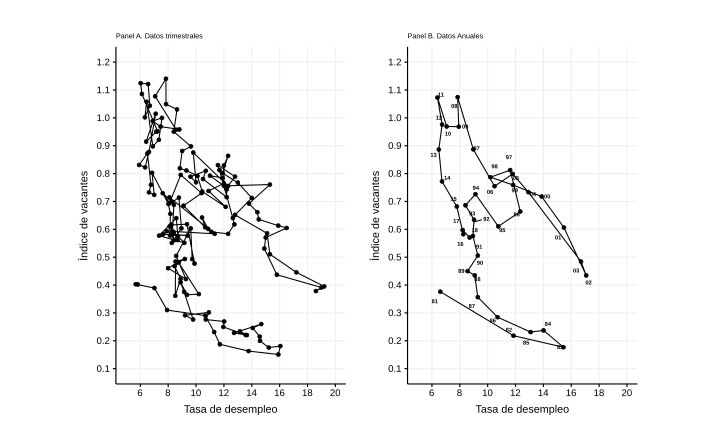
\includegraphics[width=\maxwidth]{tesis_files/figure-latex/beveridge-curve-1.pdf}
\caption{Curva de Beveridge 1981-2018}\label{fig:beveridge-curve}\textsc{}

\footnotesize\textsc{Notas} -- Curva de Beveridge 1981-2018, Montevideo. Los colores representan las décadas de 1980, 1990, 2000 y 2010. El ratio de los ejes expresado como y/x es igual a 15. Se observa una curva con pendiente negativa y traslados paralelos entre 1980 y 2000. El periodo de 1990 muestra una transición hacia un punto más alejado del origen. El periodo de 2010 muestra un traslado hacia el origen.

\textsc{Fuentes} -- Tasa de desempleo trimestral calculada por INE, índice de vacantes de elaboración propia.
\end{figure}
El primer hallazo del trabajo se observa en la Figura \ref{fig:beveridge-curve} Panel A, es una relación negativa entre vacantes y desempleo en linea con la evidencia la literatura y teoría económica. Se observa que la curva ha sufrido traslados tanto hacia afuera como hacia el origen lo que debería relacionararse a modificaciones estructurales de distinta indole o bien shocks. También parecen existir movimiento diagonales relacionados al ciclo económico.

En la Figura \ref{fig:beveridge-curve} Panel B observamos los promedio anuales del índice de vacantes y tasa de desempleo. Aquí queda un poco más claro que la década de los 80, esta en un cuadrante inferior hacia la izquierda en contraposición a la década del 2000 que es la más alejada del origen. Las observaciones de la década de los 90, se alejan del origen de forma oscilante, mientras las observaciones de los años 2010 se mueven de forma descendente y con una elevada pendiente moviendose entorno al 6-8\% de desempleo. Claramente es la década con menor variabilidad en la tasa de desempleo.
\begin{figure}
\includegraphics[width=\maxwidth]{tesis_files/figure-latex/td-vac-pib-1.pdf}
\caption{Producto-Vacantes y Producto-Desempleo (1981-2018)}\label{fig:td-vac-pib}\textsc{}

\footnotesize\textsc{Notas} -- Relación entre producto-vacantes y producto-desempleo, datos desde 1981 hasta 2018. Los colores representan las décadas de los años 1980 hasta 2010. La relación de los ejes medidos como y/x son respectivamente 1/70 y 1/6. En el panel A se observa el producto y el índice de vacantes, hasta el año 2012 la correlación es positiva, luego negativa. En el panel B observamos el producto y la tasa de desempleo. Las décadas de 1980 y 2000 muestran un comportamiento similar, una forma de U que hace referencia las crisis de 1982 y 2002.

\textsc{Fuentes} -- Tasa de desempleo corresponde a publicaciones trimestrales de INE. La serie de producto es elaborada por el BCU, la misma fue facilitada por CINVE. Índice de vacantes de elaboración propia.
\end{figure}
En la Figura \ref{fig:td-vac-pib} Panel A podemos observar la relación entre vacantes y PIB. En la década de 2010 hay una notoria caída de vacantes laborales que no se ve acompañada por el PBI, como puede observarse en los años 80 y 2000. La correlación entre PIB y vacantes se torna negativa a partir del año 2012. La tasa de variación negativa en que caen las vacantes laborales entre 2011 y 2018, es prácticamente la misma entre 1998-2002 y 1981-1983, sin embargo el nivel de actividad no cae en ningún momento por lo que no se observa el movimiento de U típico de 80-82 y 98-2002.

En la Figura \ref{fig:td-vac-pib} panel B observamos el mismo comportamiento de la CB en los años 90, una transición hacia un nuevo estado desde una década de crecimiento con alto desempleo, hacia otra con crecimiento y caída del desempleo, los años 2000. Además, los 80 y 2000 vuelven a compartir la forma de U, solo que esta vez es en sentido contrario. La década de 2010 muestra a diferencia del gráfico anterior un comportamiento similar a los 90, observandose crecimiento económico con crecimiento del desempleo, aunque el nivel de actividad no cae en ningún momento.

\hypertarget{quiebres-estructurales-1}{%
\section{Quiebres estructurales}\label{quiebres-estructurales-1}}

A continuación, ponemos a prueba la hipótesis de existencia de algún quiebre estructural en la relación vacantes y desempleo y buscamos, en caso de existir, la fecha de dichos quiebres.

Planteamos:
\begin{equation}
log(ind\_vac_i) = \beta_i + \beta_i\log(td_i) + \epsilon_i
\end{equation}
Y sometemos a prueba:
\begin{align}
H_0: \beta_i &= \beta_0 \ \ \ (i = 1, ..., n) \\
H_1: \beta_i &\not= \beta_0 \ \ \ (i = 1, ..., n)
\end{align}
Los resultados se pueden ver en el Cuadro \ref{tab:quiebres}, donde se han llevado a cabo los test de fluctuación generalizada. En la columna \emph{Test}, se identifican los test de quiebres estructural llevados a cabo siguiendo la nomenclatura usada por Zeileis et al. (\protect\hyperlink{ref-Zeileis2002}{2002}). La diferencia entre Rec-CUSUM y Rec-CUSUM(d) es que se permite la existencia de un rezago, ya que, Kramer et al. (\protect\hyperlink{ref-Society1988}{1988}) muestran que los test CUSUM no pierden sus propiedades al relajar algunos supuestos, como trabajar con modelos dinámicos. En todos los casos que no se utilizan rezagos de la tasa de vacantes, se rechaza la hipótesis nula de invariabilidad en los parámetros, por tanto, no se rechaza la existencia de algún quiebre estructural en la relación entre vacantes y tasa de desempleo. Los únicos test que no rechazan \(H_0\) son Score-CUSUM y OLS-CUSUM(d) modelos que incluyen un parámetro autoregresivo de vacantes. En todos los casos, siguiendo a Zeileis (\protect\hyperlink{ref-Zeileis2004}{2004}) se estimo la matriz de varianzas y covarianzas robusta ante la heteroscedasticidad y autocorrelación usando un estimador de kernel cuadrático HAC (Andrews, \protect\hyperlink{ref-Andrews1991}{1991}) con un filtrado VAR(1) y una elección automática del ancho de banda basado en una aproximación AR(1)\footnote{El kernel génerico es \(\omega_l = K(\frac{l}{B})\) con K la función de kernel y B el ancho de banda. El kernel espectral tiene la siguiente forma \(\omega_l = \frac{3}{z^2}(\frac{\sin(z)}{z} - \cos(z))\) siendo \(l\) el rezago y \(z = \frac{6\pi}{5}\frac{l}{B}\), ver Andrews (\protect\hyperlink{ref-Andrews1991}{1991})}.

En las Figuras de la sección \ref{efpAnexo} en el apéndice podemos observar las fluctuaciones del proceso empírico y su comparación con la fluctuación del proceso límite. Esto muestra en que periodo debería estar el o los quiebres en los parámetros, básicamente todos los test utilizados en el Cuadro \ref{tab:quiebres} comparten que la hipótesis nula de la no existencia de cambio estructural debería ser rechazada cuando el proceso empírico se vuelve improbablemente superior a las fluctuaciones del proceso límite (Zeileis et al., \protect\hyperlink{ref-Zeileis2002}{2002}).

Los test Score permiten observar variabilidad en la varianza, al sobrepasar el umbral esta es estadísticamente signifiticativa al 5\%. Tanto en el test Score-CUSUM como Score-MOSUM la varianza muestra fluctuaciones entre 1990 y 1995, y en torno a 2010-2011, sobrepasando el umbral. Por otra parte, el test Score-CUSUM con rezagos con p-valor 0.5, muestra una varianza al límite del umbral, pero sin sobrepasarlo. Es un indicio de que es posible plantear un modelo que no solo tome en cuenta los quiebres en la media condicional sino también en la varianza de los errores lo cual puede mejorar la estímación de los quiebres (Bai \& Perron, \protect\hyperlink{ref-BaiPerron2003}{2003}), por ello se estiman modelos de quiebres tanto de parámetros como varianza siguiendo a Zeileis et al. (\protect\hyperlink{ref-Zeileis2010}{2010}).

Planteamos los test de tipo F generalizados definiendo el tamaño mínimo del intervalo a considerar, en base a un parámetro de ancha de banda, h fijado en 0.15.

Utilizamos las tres variaciones propuestas por Andrews (\protect\hyperlink{ref-Andrews1993}{1993}) y Andrews \& Ploberger (\protect\hyperlink{ref-Andrews1994}{1994}), supF, aveF y expF. En el Cuadro \ref{tab:ftest} podemos observar el test, el valor del estadístico y el p-valor asociado. Se uso la misma matriz de variazas y covarianzas robusta igual que en el caso anterior. En los tres test, encontramos un quiebre estructural en torno a 1990-I, resultado en linea con Urrestarazu (\protect\hyperlink{ref-Urrestarazu1997}{1997}).



\begin{table}

\caption{\label{tab:vcovHAC-andrews}Coeficientes de cada periodo}
\centering
\resizebox{\linewidth}{!}{
\begin{threeparttable}
\begin{tabular}[t]{ccccccc}
\toprule
Periodo & Coeficiente & Estimación & Estándar error & Estadístico & p-valor & Significación\\
\midrule
1981 Q1--1990 Q2 & $\hat{\beta}_0$ & 1.33 & 0.55 & 2.41 & 0.02 & *\\
1981 Q1--1990 Q2 & $\hat{\beta}_1$ & -1.08 & 0.21 & -5.25 & 0.00 & ***\\
1981 Q1--1990 Q2 & $\hat{\sigma}^2$ & 0.03 & 0.01 & 2.66 & 0.01 & *\\
1990 Q3--1996 Q2 & $\hat{\beta}_0$ & 0.23 & 0.32 & 0.71 & 0.49 & \\
1990 Q3--1996 Q2 & $\hat{\beta}_1$ & -0.31 & 0.13 & -2.34 & 0.03 & *\\
\addlinespace
1990 Q3--1996 Q2 & $\hat{\sigma}^2$ & 0.01 & 0.00 & 2.98 & 0.01 & **\\
1996 Q3--2013 Q1 & $\hat{\beta}_0$ & 1.47 & 0.27 & 5.50 & 0.00 & ***\\
1996 Q3--2013 Q1 & $\hat{\beta}_1$ & -0.73 & 0.12 & -6.21 & 0.00 & ***\\
1996 Q3--2013 Q1 & $\hat{\sigma}^2$ & 0.01 & 0.00 & 3.06 & 0.00 & **\\
2013 Q2--2018 Q4 & $\hat{\beta}_0$ & 1.93 & 0.19 & 10.00 & 0.00 & ***\\
\addlinespace
2013 Q2--2018 Q4 & $\hat{\beta}_1$ & -1.15 & 0.09 & -12.23 & 0.00 & ***\\
2013 Q2--2018 Q4 & $\hat{\sigma}^2$ & 0.00 & 0.00 & 4.09 & 0.00 & ***\\
\bottomrule
\end{tabular}
\begin{tablenotes}
\item \textit{Notas:} 
\item \footnotesize Estimación para los cuatro periodos detectados mediante los test de quiebres estructural siguiendo a Bai \& Perron (\protect\hyperlink{ref-BaiPerron2003}{2003}) y Zeileis et al. (\protect\hyperlink{ref-Zeileis2010}{2010}). Se muestran los valores de los coeficientes estimados $\beta_0$, $\beta_1$ y $\sigma^2$ en la columna \textit{Estimación}, sus errores estándar en \textit{Estándar error} y el valor del estadístico en \textit{Estadístico}. \textit{P-valor} muestra los respectivos p-valores de cada prueba. \textit{Significación} muestra los niveles de significación donde . quiere decir no significativo al 5\% pero si al 10\%. Un * es estadísticamente significativo al 5\%, ** es significativo al 1\% mientras *** es significativo al 0.1\%. En todos los casos los coeficientes son estadísticamente significativos al 5\% a excepción de $\beta_0$ entre 1990 y 1996. Los signos de $\beta_1$ son negativos para todos los períodos. En el período 2013 el valos de $\sigma^2$ es diferente de 0, pero ha sido redondeado.
\end{tablenotes}
\end{threeparttable}}
\end{table}
Finalmente, pasamos a calcular todos los posibles periodos de quiebres estructurales de forma generalizada. Para ello se siguen los trabajos de Bai \& Perron (\protect\hyperlink{ref-BaiPerron2003}{2003}), Bai \& Perron (\protect\hyperlink{ref-BaiPerron1998}{1998}) y aplicaciones de Zeileis, Kleiber, Walter, \& Hornik (\protect\hyperlink{ref-Zeileis2003}{2003}), en especial a Zeileis et al. (\protect\hyperlink{ref-Zeileis2010}{2010}). Obtenemos tres quiebres estructurales en los años 1990-II, 1996-II y 2013-II usando como función objetivo la log-verosimilitud negativa.\footnote{Los quiebres son exactamente iguales si las variables se modelan en niveles o logaritmos. Es posible modelar otro cambio estructural eligiendo otra función objetivo como el BIC o RSS, sin embargo dicho intervalo es extremadamente amplio al computarlo con una matriz HAC, al elegir un máximo de 3 puntos de quiebres se obtienen los mismos resultados, si se fija un máximo de 4 se obtiene un quiebre adicional en 2004-I y se mantienen los restantes.} Por lo tanto, los 4 periodos de análisis son 1981-I.1990-II, 1990-III.1996-II, 1996-III.2013-I y 2013-II.2018.IV. En el Cuadro \ref{tab:vcovHAC-andrews} observamos que en todos los periodos los parámetros muestran el signo correcto según la teoría (negativo). En todos los casos son estadísticamente significativos al 5\%, usando una matriz HAC con ponderadores de Andrews. Sin embargo, usando ponderadores de Kernel en el segundo periodo el p-valor es 0.12. Dada la existencia de autocorrelación y heteroscedasticidad, la elección de la matriz de ponderadores es relevante y puede generar variaciones en la significatividad estadística de algunos parámetros. Por ello los Cuadros \ref{tab:vcovHAC-lumley}, \ref{tab:kernHAC} y \ref{tab:NeweyWest} muestran diferentes ponderaciones para los distintos periodos. Es de notar que el único momento que podría ser discutible es entre 1990-III.1996-II, en el cual dependiendo la elección de la matriz el parámetro de la tasa de desempleo puede resultar no significativo, sin embargo, si se estima para el mismo periodo un modelo lineal pero sin varianza de los errores, la tasa de desempleo es estadísticamente significativa, con el signo del coeficiente negativo. En el resto de los casos los coeficientes son estadísticamente significativos al nivel \(\alpha = 0.05\), al igual que las varianzas de cada periodo.

Las CB estimadas para los periodos obtenidos se pueden ver en la Figura \ref{fig:BCtest}. En todos los casos se mantiene una relación negativa entre vacantes y desempleo. A la vez que se observan cambios de nivel y pendiente. El primer periodo desde 1981-I hasta 1990-II muestra una curva comparativamente más cercana al origen que 1990-III a 1996-II donde se traslada de forma paralela, lo mismo vuelve a suceder en 1996-III a 2013-II (incluyendo un leve cambio de pendiente). El comportamiento se modifica a partir de 2013-III en donde la curva tiene un cambio tanto paralelo como de pendiente hacia el origen.
\begin{figure}
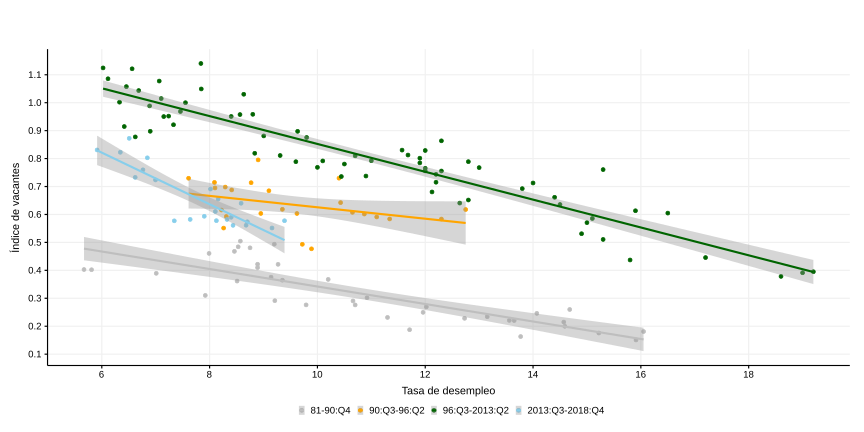
\includegraphics[width=\maxwidth]{tesis_files/figure-latex/BCtest-1.pdf}
\caption{Curva de Beveridge por periodo}\label{fig:BCtest}\textsc{}

\footnotesize\textsc{Notas} -- CB para los periodos obtenidos mediante los test de quiebre estructural siguiendo a Zeileis et al. (\protect\hyperlink{ref-Zeileis2010}{2010}) y Bai \& Perron (\protect\hyperlink{ref-BaiPerron2003}{2003}). Se utiliza el paquete fxregime, resultados similares se obtienen con strucchange. En todas las etapas, la relación entre vacantes y desempleo es negativa. Se observan traslados de la CB y movimientos de pendiente. La segunda época entre los años 90-96 muestra un traslado hacia fuera, lo mismo sucede entre 96-2013. PEn 2013-2018 se da un corrimiento al origen, indicios de un mercado laboral que podría ser más eficiente.

\textsc{Fuentes} -- Datos de vacantes laborales de elaboración propia. Tasa de desempleo obtenida de INE.
\end{figure}
\hypertarget{tvp-var-1}{%
\section{TVP-VAR}\label{tvp-var-1}}

Por último, realizamos una estimación multivariada de un vector autoregresivo con parámetros variables y volatilidad estocástica siguiendo a Primiceri (\protect\hyperlink{ref-Primiceri2005}{2005}), Lubik \& Matthes (\protect\hyperlink{ref-Lubik2016}{2016}) y Lubik \& Matthes (\protect\hyperlink{ref-Lubik2016b}{2015}), usando el algoritmo corregido por Del Negro \& Primiceri (\protect\hyperlink{ref-DelNegro2015}{2015}). Nos interesa analizar la variabilidad en los parámetros beta y la matriz de varianzas y covarianzas, sumado al efecto de un shock por parte del producto sobre vacantes y desempleo.

Usamos las primeras 36 observaciones, nueve años, desde 1981-I hasta 1989-IV para calibrar las distribuciones a priori, quedando un periodo efectivo desde 1990 hasta 2018. Simulamos 50 mil veces y elegimos un orden de rezagos igual a uno, es decir, un TVP-VAR(1).\footnote{Se corrieron 50 mil simulaciones con un orden de rezagos igual a dos y los resultados fueron los mismos. Por ello, se muestra un TVP-VAR(1) en la medida que se facilita la visualización.} Las series utilizadas de producto, tasa de desempleo e índice de vacantes son todas de frecuencia trimestral, lo cual (a excepción del PIB que se publica trimestralmente) va a generar series con menor variabilidad.

La restricción de identificación es que son los shocks desde el producto (shocks de productividad) los cuales afectan al desempleo y las vacantes laborales, con un rezago. Por lo tanto, el orden de exogeneidad de las variables es que el pib es la primer variable, seguido del índice de vacantes y la tasa de desempleo. El orden de la segunda y tercer variable, no es una restricción de identificación sino una normalización necesaria que puede modificar los resultados (Primiceri, \protect\hyperlink{ref-Primiceri2005}{2005}), sin embargo, en este caso el orden no genera diferencias. La estructura de identificación elegida para las innovaciones es básicamente una especificación de Cholesky. En la Figura \ref{fig:svar-parameters} observamos los desvíos estandar variables a lo largo del tiempo de los residuos del modelo, se gráfica la media (posterior) y los cuantiles 16 y 84\footnote{Normalidad}.

El gráfico muestra dos resultados, el primero es que las vacantes laborales son estables para el periodo. El segundo es que si bien la magnitud es leve, parecen existir dos periodos desde 1990 hasta 2005 y desde 2005 en adelante con una transición suave, donde el primero presenta una mayor varianza tanto para el pib como la tasa desempleo, mientras en el caso de las vacantes no se observan diferencias.\footnote{En los test de quiebre estructural si se definen cuatro posibles quiebres estructurales, el cuarto se genera en torno a 2004.} Las modificaciones en las varianzas comienzan previo a 2005, lo cual se relaciona con la crisis de la economía en 2002 y el posterior crecimiento ininterrumpido a partir del tercer trimestre de 2003.
\begin{landscape}
\begin{figure}
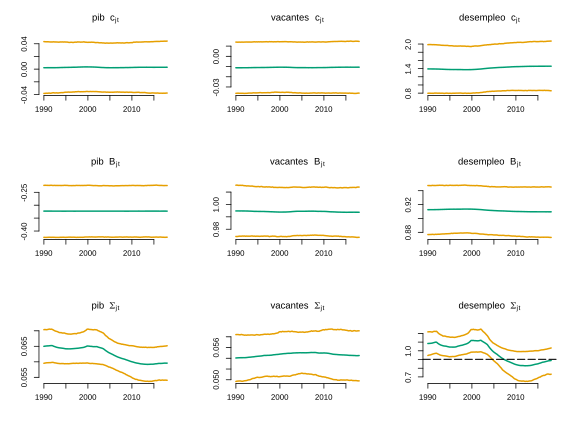
\includegraphics[width=\maxwidth]{tesis_files/figure-latex/svar-parameters-1.pdf}
\caption{Media posterior y volatilidades modelo TVP-VAR}\label{fig:svar-parameters}\textsc{}

\footnotesize\textsc{Notas} -- Se grafica las matrices $\hat{A}_{jt}$ y $\hat{\Sigma}_{jt}$ desde 1990 hasta 2018 para el producto, índice de vacantes y tasa de desempleo. Observamos los desvíos estandar de los residuos del modelo, la media (posterior) y los cuantiles 16 y 84. Parecen existir dos periodos desde 1990 hasta 2005 y desde 2005 en adelante, donde el primero presenta mayor varianza tanto para el pib como la tasa desempleo. En las vacantes, no se observan diferencias.

\textsc{Fuentes} -- Serie de producto facilitada por CINVE. Tasa de desempleo obtenida de INE. Índice de vacantes construcción propia.
\end{figure}
\end{landscape}
En la Figura \ref{fig:svar-parameters} se puede observar que los parámetros variables rezagados \(B_{j,t}\) y los interceptos \(c_{t}\) tienen poca variabilidad a lo largo del periodo de análisis\footnote{se muestra la estimación de un TVP-VAR(1) en vez de un TVP-VAR(2), dado que los resultados no se modifican y se facilita su visualización}. Este resultado es común en la literatura de TVP-VAR (Lubik \& Matthes, \protect\hyperlink{ref-Lubik2016b}{2015}), sin embargo, como se noto en el párrafo anterior si existe variabilidad en las innovaciones.

El resultado es robusto frente a diferentes especificaciones, con variables en niveles o en logaritmos los resultados no cambian. Adicionalmente se estimo un modelo bivariado con desempleo y vacantes, tanto en niveles como en logaritmos, obteniendo las mismas conclusiones. Se podría pensar en el uso de un modelo de parámetros fijos y volatilidad estocástica, sin embargo, en la medida que el TVP-VAR no impone la restricción de parámetros fijos pero se obtiene dicho resultado no parece necesario.
\begin{figure}
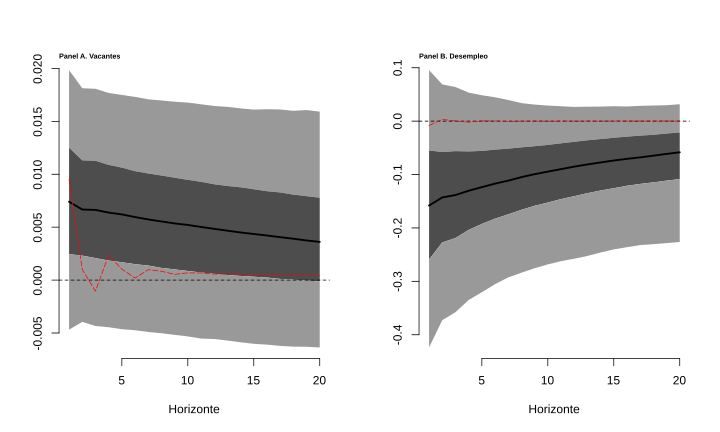
\includegraphics[width=\maxwidth]{tesis_files/figure-latex/FIR-1.pdf}
\caption{FIR}\label{fig:FIR}\textsc{}

\footnotesize\textsc{Notas} -- FIR desde producto hacia el índice de vacantes (A) y tasa de desempleo (B). La linea negra es la mediana, mientras las áreas grises refieren a los intervalos de confianza al 5-95\% y 25-75\%. Con color rojo la FIR de un VAR de parámetros fijos. Los signos de la mediana del TVP-VAR se ajusta a lo que se espera de un shocks desde el producto a vacantes y desempleo. En el primer caso un efecto positivo y en el segundo un efecto negativo. En el caso de un VAR los resultados son menos claro con valores en torno a cero.

\textsc{Fuentes} -- Serie de producto facilitada por CINVE. Tasa de desempleo obtenida de INE. Índice de vacantes construcción propia.
\end{figure}
Por último analizamos las FIR mediante la estimación de la mediana. Su visualización no es trivial, en la medida que en cada momento del tiempo existe una FIR. Una opción es visualizar distintos momentos y observar si existen diferencia (la que se elige), otra es mostrar una visualización en tres dimensiones. En nuestro caso, las FIR en los distintos momentos del tiempo se mantienen prácticamente iguales.

En la Figura \ref{fig:FIR} Panel A tenemos shocks desde el producto hacia las vacantes laborales el efecto es positivo en todo momento, esto tiene sentido en la medida que una innovación de productividad, debería generar que la demanda laboral de las empresas se vea aumentado, en la medida que crezca el nivel de producción de la economía. Al contrario en la Figura \ref{fig:FIR} Panel B observamos como el efecto del shock genera un efecto negativo en todo momento sobre la tasa de desempleo. Al mejorar la productividad de la economía, el desempleo debería disminuir en la medida que la economía es capaz de aumentar su producción, lo cual lleva a que las empresas aumenten su contratación (más o menos dependiendo de cuan sesgado sea hacia el uso de tecnología y capital). Los efectos de entrada o salida de personas a la PEA esta presente en ambos indicadores.

\hypertarget{cap:Discusion}{%
\chapter{Discusión}\label{cap:Discusion}}

\hypertarget{indicador}{%
\section{Indicador}\label{indicador}}

El índice de vacantes construido esta sujeto a comentarios y futuras mejoras, tanto en lo que refiere a las fuentes de información, los métodos de imputación utilizados así como la metodología utilizada para calcular y combinar las diferentes series individuales. Por ejemplo, en lo referido a la información la serie construida es de avisos laborales no de puestos de trabajo. En la medida que los puestos sigan una dinámica diferente que los avisos estaríamos representando incorrectamente la demanda laboral por parte de las empresas. Para corroborar este punto, se llevan a cabo dos pruebas: a) entre 1996 y 1998, se contabilizan todos los puestos publicados en la sección de avisos destacados.\footnote{No se contabilizan los avisos publicados en otras secciones por un tema de tiempo. Por lo cual, se asume que los avisos en dichas secciones corresponden a un puesto} En la Figura \ref{fig:molina96-98} se observa que puestos y avisos se mueven de forma conjunta, manteniendo una diferencia de nivel. b) Entre los años 2000 y 2009, se cuenta con la base de datos proporcionada por IECON. Dicha base surge del trabajo de Espino et al. (\protect\hyperlink{ref-Alma2011}{2011}) en el cual contabilizan todos los avisos y puestos laborales en las primeras 2 semanas de los meses 3, 5 o 6 y 9 de los respectivos años. En la Figura \ref{fig:iecon-avisos-puestos} se puede ver que ambas tienen una diferencia de nivel.

Además, para el periodo 1998-2014 se usan datos del ICDL al cual se le extrajeron los componentes estacionales, no estando disponible la serie original y, no se tiene detalles precisos de la metodología. Sin embargo, se pudo corroborar que el ICDL corresponde, al menos hasta 2012, con los avisos laborales en papel recogidos en \emph{Gallito}. El ICDL tiene base agosto 1998, dicho mes fue contabilizado completamente lo cual permite generar una aproximación a la cantidad de puestos. A futuro es posible ampliar las muestras entre 1998 y 2014, combinar dichos datos con los obtenidos por Espino et al. (\protect\hyperlink{ref-Alma2011}{2011}), generar una subserie para el periodo 1998-2014, comparar con el ICDL y potencialmente dejar de utilizarlo. Esto permitiría recobrar el componente estacional, pero para este trabajo dicho componente no es relevante y tampoco lo es en la medida que la CB se suele analizar de forma desestacionalizada. Si lo es para tener una medida más precisa de las publicaciones laborales por si sola y lograr una mejor desestacionalización para la serie completa entre 1980 y 2019.

Otro comentario es que la serie de avisos es de Montevideo aunque contiene información de otros departamentos. Observando la Figura \ref{fig:avisos-dpto} que corresponde a todos los avisos obtenidos mediante scraping en el año 2019, se puede ver que para Buscojobs, Computrabajo y Gallito las publicaciones correspondientes a Montevideo son de 82\%, 84\% y 95\% respectivamente. Por lo tanto, se puede mantener que es representativa de la capital. Es posible suponer que el porcentaje de publicaciones no de Montevideo se mantiene estable a lo largo del periodo y reponderar la serie de avisos. Sin embargo, se opta por trabajar con todos los datos.

A los posibles sesgos de información de otros departamentos se añade que la serie de \emph{Gallito} presenta un sesgo hacia puesto de baja calificación. En la Figura \ref{fig:ga13-18-comparacion} se observa que la mayor cantidad de avisos corresponden a puestos de auxiliar, técnico/especialista, ejecutivo comercial y peón. Si bien, esto no es una muestra del sesgo, puesto que los puestos de mayor jerarquía son por definición menor a los puestos de menor calificación, por lo cual una simple comparación porcentual no nos dice nada. Espino et al. (\protect\hyperlink{ref-Alma2011}{2011}) utilizando la información de puestos laborales para el periodo 2000-2009, utilizando la misma fuente de datos realizan un análisis pormenorizado de la información publicada en cada aviso laboral y lo comparan con la ECH, concluyendo que \emph{Gallito} tiene sesgo hacia puestos de baja calificación. Es posible extender el análisis de Espino et al. (\protect\hyperlink{ref-Alma2011}{2011}) y replicarlo para el periodo 2013-2018. Lo mismo puede realizarse para el año 2019 con la información recolectada en \emph{Buscojobs} y \emph{Computrabajo}.

Un punto marcado por Rama (\protect\hyperlink{ref-Rama1988}{1988}) es que la existencia de informalidad es una característica propia de los países subdesarrollados a la cual Uruguay no escapa. Ello se agrava para los años entre 1980 y 2005, debido a las graves crisis económicas de 1982 y 2001-2002. Las vacantes laborales publicadas en la prensa no captan los puestos generados en la informalidad. Una posible solución sería estimar la informalidad para el periodo considerado y ajustar una nueva serie de vacantes que tome en cuenta dicho factor.

¿Cuán representativo es un índice de vacantes laborales respecto de la demanda laboral? Se puede argumentar que tomar las vacantes laborales no es representativo de la demanda laboral. Sin embargo, Barnichon (\protect\hyperlink{ref-Barnichon2010}{2010}) construye un índice de vacantes utilizando tanto fuentes de avisos laborales en la prensa, como encuestas a empresas realizadas por el Bureu of Labor Statistics mediante el Job Openings and Labor Turnover Survey (JOLTS). Encuentra que las series siguen la misma dinámica, aunque la serie de JOLTS necesita ser reescalado.

Por último, si bien la serie de vacantes tiene una correlación positiva con el PIB para el periodo 1980-2019, se correlaciona negativamente si se toma desde 2013 en adelante. Esto genera dudas importantes sobre su construcción en los últimos cinco años. Sin embargo, aún si se sumaran de forma bruta todos los avisos recolectados de \emph{Gallito}, \emph{Computrabajo} y \emph{Buscojobs} la correlación negativa se mantiene. Vale recordar que \emph{Buscojobs} contiene la información publicada en el portal \emph{Uruguay Concursa}, por lo cual son cuatro fuentes de datos relevantes. Esto puede verificarse en base a las encuestas del uso de Internet realizadas por Cifra, en base a los datos recolectados las páginas más utilizadas por las personas que buscan trabajo son las utilizadas en este trabajo, a excepción de \emph{LinkedIn}. Es inverosímil pensar que agregando \emph{LinkedIn} cambie de forma tan relevante la dinámica de los avisos, en especial porque dicha página levanta publicaciones de los cuatro portales utilizados en este trabajo. Una potencial explicación es que el PIB mantiene su base 2005, lo cual genera que el sector Telecomunicaciones tenga un crecimiento exponencial al ser valuado a precios de 2005. Al modificar la base es posible que esto tenga un efecto importante y altere las estimaciones actuales del producto. Otra posible explicación es que la economía este pasando por un cambio importante en el cual pese al crecimiento las firmas demandan cada vez menos puestos laborales, en la medida que sustituyen trabajo por capital y utilizan nuevos procesos de producción. Si se añade que la serie principal de este trabajo, \emph{Gallito}, tiene sesgo hacia puestos de baja calificación (Espino et al., \protect\hyperlink{ref-Alma2011}{2011}) y estos son los más afectados por los nuevos procesos de producción y prestación de servicios, el efecto de crecimiento con menos solicitudes laborales se potencia.

\hypertarget{estimaciones}{%
\section{Estimaciones}\label{estimaciones}}

El resultado obtenido en la estimación TVP-VAR es común en la literatura de esta estrategia, la posibilidad de no encontrar variabilidad en intercepto y rezagos pese a que si debería existir y, si encontrar quiebres en las varianzas y covarianzas, sumado a la sensibilidad dada la elección de los priors (Lubik \& Matthes, \protect\hyperlink{ref-Lubik2016b}{2015}). Esto se agrava al trimestralizar la serie de desempleo y vacantes laborales, ya que se pierde variabilidad. Es posible calcular a partir de 1996 las vacantes de forma mensual, por lo cual sería interesante realizar un análisis bivariado desde 1996 en adelante entre vacantes y desempleo. También podría realizarse un análisis similar al de Lubik \& Matthes (\protect\hyperlink{ref-Lubik2016b}{2015}) y ver cuan sensible es la estimación a la elección de priors. Por último, debe notarse una leve disminución en la matriz de varianzas y covarianzas de producto y desempleo en torno a 2005 lo cual parece indicar dos etapas que coinciden con la salida de la crisis económica de 2002 y un periodo de alto crecimiento económico y bajo desempleo, cambios asociados al ciclo económico y un auge de commodities. En la medida que un TVP-VAR con volatilidad estocástica es una forma reducida de un DSGE, esto podría dar indicio de dos períodos diferentes a evaluar bajo dicha metodología. Por último, puede ser posible que las series no tengan quiebres continuos y si discretos, como se obtuvo, aunque esto es un tanto dudoso en la medida que no se rechaza la raíz unitaria de la serie de vacantes (ni de las sub series de vacantes) y desempleo como puede observarse en el Cuadro \ref{tab:test-ru-trim}.

A continuación nos centramos el los resultados de los quiebres estructurales, donde obtenemos 4 o 5 periodos de tiempo dependiendo si los quiebres se eligen utilizando el BIC o BIC corregido. Lo importante es que los quiebres previos no se modifican si se permite uno adicional. Los resultados indican distintas fases de la CB que pueden deberse a cambios por el ciclo económico (dadas las crisis y periodos de alto y bajo crecimiento o alteraciones de la PEA) como a factores estructurales de distinta índole como institucional, tecnológico o un \emph{mismatch} de habilidades.

El factor institucional debería jugar un factor relevante en los traslados de la CB resultado en linea con Nickell et al. (\protect\hyperlink{ref-Nickell2002}{2002}), Gujarati (\protect\hyperlink{ref-Gujarati1972}{1972}) y Bouvet (\protect\hyperlink{ref-Bouvet2012}{2012}). Comenzamos con el periodo 80-90 y 90-96. La década de los 80 se caracteriza por una elevada negociación por rama empresarial, en contraposición a la negociación por empresa en los 90, adicionalmente cae la sindicalización donde la cantidad de afiliados a sindicatos privados se reduce a la mitad en la medida que se dejo de convocar a partir de 1992 a los consejos de salarios. Sin embargo, también hay una importante ganancia de productividad en los 90, sumado a una caída de las horas trabajadas, desempleo elevado constantemente, aumento de la informalidad al aumentar la proporción de ocupados en el sector servicios y caída de trabajadores en el sector manufacturero y alto crecimiento hasta 1998. Aunque dicho crecimiento fue fomentado por la apertura de la economía uruguaya tanto de cuenta corriente como de capitales, la cual propicio que las empresas locales no fuesen capaces de competir con los productos importados y se vieran obligadas a cerrar (Antía, \protect\hyperlink{ref-Antia2001}{2001}), lo cual puede verse como shocks sectoriales al igual que los analizados por Blanchard \& Diamond (\protect\hyperlink{ref-Blanchard1989}{1989}), o shocks comunes como en Benati \& Lubik (\protect\hyperlink{ref-Benati2013}{2013}), lo cual no sería raro dado los shocks de crisis de tequila, crisis asiática y devaluación brasileña. Otra opción es pensar que las transformaciones económicas de los 90 generaron una disminución en la eficiencia del matching, similar a la planteada por Lubik (\protect\hyperlink{ref-Lubik2013}{2013}).

El traslado de la CB hacia el periodo 1996 a 2013 podemos pensar que fue debido a las políticas aplicadas en la primera mitad de los 90 propiciando una CB más alejada del origen, que podría ser un mercado con menos eficiencia. Y que los movimientos sobre la curva deberían estar dados por el ciclo económico, el cual tiene su etapa recesiva entre 1998 y 2003 y una fase fuertemente expansiva entre 2004 y 2012, dicha interpretación se ajusta a la tasa de crecimiento del producto y el bajo desempleo observado, es un shock de oferta agregada como en Blanchard \& Diamond (\protect\hyperlink{ref-Blanchard1989}{1989}). También podemos pensar en los desplazamientos de la fuerza laboral que pueden reducir la eficiencia del matching (Hobijn \& Şahin, \protect\hyperlink{ref-Hobijn2013}{2013}), el más notorio es la caída de la PEA en torno a 2004, movimiento demográfico dado por la crisis de 2002 que podrían alterar la CB (Bewley, \protect\hyperlink{ref-Bewley1979}{1979}). Sin embargo no hay que olvidar la cantidad de reformas estructurales, las cuales aumentaron el salario mínimo, convocan los consejos de salarios, fomentan la negociación por rama de actividad, regulan el trabajo del servicio doméstico, aprueban la ley de responsabilidad penal empresarial (Bergara \& Milnitsky, \protect\hyperlink{ref-Bergara2017}{2017}) y se da que la central obrera PIT-CNT cuadruplica sus afiliados entre 2005 y 2020. Son todos factores similares a los encontrados por Bouvet (\protect\hyperlink{ref-Bouvet2012}{2012}) y Nickell et al. (\protect\hyperlink{ref-Nickell2002}{2002}).

Por último, el traslado hacia el origen de la CB en 2013 podría deberse a cambios en los procesos de contratación, resultado observado por Elsby et al. (\protect\hyperlink{ref-Elsby2015}{2015}). Recordemos que a partir de 2008 los portales laborales comienzan a tener un flujo de avisos relevante, a la vez que aumenta sistemáticamente la penetración de Internet en los hogares. Dada la enorme caída en el índice de vacantes y el aumento leve del desempleo relativo a sus valores históricos, no debería ser extraño que la eficiencia del matching haya aumentado considerablemente guiado en parte por la disminución en el tiempo de búsqueda tanto del empleador como trabajador. Además, las reformas institucionales que han favorecido al trabajador deberían tener un efecto negativo en la medida que funcionan como un aumento de las fricciones, sin embargo en 2013 la curva se traslada hacia el origen, lo cual fortalece la hipótesis de que los procesos de contratación han generado una mejora del matching.

En conclusión, si bien las factores institucionales deberían estar jugando un papel relevante en los traslados de la CB, no es menos cierto que han habido modificaciones importantes asociadas a factores tecnológicos y factores de ciclo económico, especialmente en los últimos veinte años. Por lo cual, no es posible responder cual debería ser la causa detras de los movimientos de la CB.

\hypertarget{cap:Conclusiones}{%
\chapter{Conclusión}\label{cap:Conclusiones}}

Este trabajo ha creado una base de datos de cantidad de avisos laborales, con la cual se calcula un índice de vacantes laborales que busca reflejar la demanda laboral por parte de las empresas en Montevideo, en la medida que la capital concentra cerca del 50\% de la población y una parte importante de la producción la misma debería ser representativa de los movimientos de vacantes a nivel Nacional. Se ha logrado generar una serie desde 1980-I hasta 2019-IV siendo la única serie de vacantes laborales actualizada en Uruguay. Se ha escrito el código en lenguaje \emph{R}, código público y reproducible, para poder obtener la información de avisos laborales futuros, lo cual da pie a que el periodo de análisis se pueda seguir extendiendo de forma ininterrumpida, aumentado las fuentes de datos y dotando de una herramienta clave como la Curva de Beveridge a la política económica.

Es de interés que el índice de vacantes construido sea perfeccionado en trabajos futuros o se intente aplicar otras metodologías (por ejemplo Barnichon (\protect\hyperlink{ref-Barnichon2010}{2010})), se agreguen nuevas fuentes de información (como Linkedin) y se mejoren datos previos. En especial durante el periodo de 2000 a 2012 en el cual se utiliza una serie filtrada sin conocimiento detallado de la transformación aplicada. Adicionalmente, es posible reducir la frecuencia de las series de trimestral a mensual. O yendo aún más lejos, la serie de vacantes podría llegar a ser semanal y que se pruebe su utilidad como un indicador adelantado de la actividad.

Una vez perfeccionado el indicador, se podría calcular tanto la tendencia como el ciclo de la serie de vacantes mediante la aplicación del filtro de Hamilton y hacer un análisis conjunto con PIB y desempleo en el dominio de frecuencias, para poder analizar en que etapa del ciclo se encuentra el proxy de la demanda laboral.

Es de hacer notar que las caídas observadas en las vacantes laborales son de orden similar a las observadas en 1982 y 2002, sin embargo la tasa de desempleo en ningún momento ha llegado a niveles similares. La única forma en que la economía soporte tal nivel de caída en la demanda laboral, es que el matching en el mercado laboral haya aumentado de forma considerable. El factor institucional es imposible no este presente dada la cantidad de reformas de caracter estructural y modificaciones en las instituciones del mercado laboral. Pero no es el único, ademas de los factores cíclicos, un factor posiblemente relevante, son los portales laborales de Internet y el avance tecnológico que permiten una búsqueda y proceso de contratación a una velocidad comparativamente mayor que los procesos iniciados mediante la prensa en papel. Las agencias de contratación (y los mismos portales) pueden manejar enormes volúmenes de información sobre posibles candidatos que permiten una búsqueda sobre un universo mayor e incluso de forma selecta. Sería interesante, agregar al trabajo un análisis sobre los flujos laborales para poder corroborar la mejora en el proceso de matching.

Por último, utilizando la metodología TVP-VAR no observamos modificación en los parámetros asociados a la media condicional y las modificaciones en las matrices de varianzas y covarianzas son leves o nulas. Sin embargo, las FIR por un shock del producto a vacantes y desempleo tiene efectos significativos. La lectura sería que los traslados paralelos observados de la CB se deben a shocks con efectos significativos de signo opuesto. Si bien la economía ha tenido fuertes shocks externos, dada la cantidad de reformas que pueden catalogarse de estructurales, sería llamativo que la variabilidad en vacantes y desempleo pueda deberse solamente a innovaciones.

Es posible profundizar sobre los modelos TVP-VAR, haciendo un análisis de priors y sus efectos, a la vez que probar y/o combinar diferentes restricciones de identificación y realizar el análisis con las series mensuales.

Finalmente es de interés para la política económica identificar cuales son las causas que están detrás de los traslados de la CB en la medida que se puedan tomar acciones para mejorar la eficiencia del mercado laboral. Por lo que es necesario que trabajos futuros investiguen al respecto.

\backmatter

\hypertarget{referencias}{%
\chapter*{Referencias}\label{referencias}}
\addcontentsline{toc}{chapter}{Referencias}

\hypertarget{refs}{}
\leavevmode\hypertarget{ref-Abraham1983}{}%
Abraham, B. K. G. (1983). Structural/Frictional vs. Deficient Demand Unemployment: Some New Evidence. \emph{American Economic Review}, \emph{73}(4), 708--724.

\leavevmode\hypertarget{ref-Abraham1987}{}%
Abraham, K. G., \& Watcher, M. (1987). Help-Wanted Advertising , Job Vacancies , and Unemployment. \emph{Brookings Papers on Economic Activity}, \emph{1987}(1), 207--248.

\leavevmode\hypertarget{ref-ArgentinaBC2019}{}%
Albertini, J., Poirier, A., \& Trupkin, D. (2019). \emph{A Job Vacancy Rate for Argentina To cite this version : HAL Id : halshs-02146600 A Job Vacancy Rate for Argentina}. Retrieved from \url{https://halshs.archives-ouvertes.fr/halshs-02146600}

\leavevmode\hypertarget{ref-Andrews1994}{}%
Andrews, B. Y. D. W. K., \& Ploberger, W. (1994). Optimal Tests when a Nuisance Parameter is Present Only Under the Alternative, \emph{62}(6), 1383--1414.

\leavevmode\hypertarget{ref-Andrews1991}{}%
Andrews, D. W. .. K. .. (1991). Heteroskedasticity and Autocorrelation Consistent Covariance Matrix Estimation. \emph{Econometrica}, \emph{59}(3), 817--858.

\leavevmode\hypertarget{ref-Andrews1993}{}%
Andrews, D. W. K. (1993). Tests for Parameter Instability and Structural Change With Unknown Change Point. \emph{Econometrica}, \emph{61}(4), 821--856.

\leavevmode\hypertarget{ref-angel2000}{}%
Angel, E. (2000). \emph{Interactive computer graphics : A top-down approach with opengl}. Boston, MA: Addison Wesley Longman.

\leavevmode\hypertarget{ref-angel2001}{}%
Angel, E. (2001a). \emph{Batch-file computer graphics : A bottom-up approach with quicktime}. Boston, MA: Wesley Addison Longman.

\leavevmode\hypertarget{ref-angel2002a}{}%
Angel, E. (2001b). \emph{Test second book by angel}. Boston, MA: Wesley Addison Longman.

\leavevmode\hypertarget{ref-Antia2001}{}%
Antía, F. (2001). \emph{La economía uruguaya en 1985-2000: políticas económicas, resultados y desafíos}. Uruguay: Instituto de Economía, Facultad de Ciencias Económicas y Administración, Universidad de la República.

\leavevmode\hypertarget{ref-Bai1997}{}%
Bai, J. (1997). Estimation of a Change Point in Multiple Regression Models. \emph{Review of Economics and Statistics}, \emph{79}(4), 551--563. \url{http://doi.org/10.1162/003465397557132}

\leavevmode\hypertarget{ref-BaiPerron1998}{}%
Bai, J., \& Perron, P. (1998). Estimating and Testing Linear Models with Multiple Structural Changes. \emph{Econometrica}, \emph{66}(1), 47--78.

\leavevmode\hypertarget{ref-BaiPerron2003}{}%
Bai, J., \& Perron, P. (2003). Computation and analysis of multiple structural change models. \emph{Journal of Applied Econometrics}, \emph{18}(1), 1--22. \url{http://doi.org/10.1002/jae.659}

\leavevmode\hypertarget{ref-Barnichon2010}{}%
Barnichon, R. (2010). Building a composite Help-Wanted Index. \emph{Economics Letters}, \emph{109}(3), 175--178. \url{http://doi.org/10.1016/j.econlet.2010.08.029}

\leavevmode\hypertarget{ref-Barnichon2012}{}%
Barnichon, R., Elsby, M. W. L., Hobijn, B., \& Şahin, A. (2012). Monthly Labor Rewiew. \emph{Monthly Labor Review}, \emph{135-6}(September), 25--37.

\leavevmode\hypertarget{ref-Benati2007}{}%
Benati, L. (2007). Drift and breaks in labor productivity. \emph{Journal of Economic Dynamics and Control}, \emph{31}(8), 2847--2877. \url{http://doi.org/10.1016/j.jedc.2006.11.004}

\leavevmode\hypertarget{ref-Benati2013}{}%
Benati, L., \& Lubik, T. A. (2013). \emph{Working Paper Series The Time-Varying Beveridge Curve The Time-Varying Beveridge Curve}. The Federal Reserve Bank of Richmond.

\leavevmode\hypertarget{ref-Bergara2017}{}%
Bergara, M., \& Milnitsky, S. (2017). Uruguay: Incentivos e instituciones en una década de reformas. \emph{El Trimestre Económico}, \emph{85}(337), 5. \url{http://doi.org/10.20430/ete.v85i337.658}

\leavevmode\hypertarget{ref-Beveridge}{}%
Beveridge. (1944). \emph{William\_Beveridge\_Full-Employment.pdf} (pp. 1--429). Londres.

\leavevmode\hypertarget{ref-Bewley1979}{}%
Bewley, R. A. (1979). The dynamic behaviour of unemployment and unfilled vacancies in Great Britain: 19581971. \emph{Applied Economics}, \emph{11}(3), 303--308. \url{http://doi.org/10.1080/758531542}

\leavevmode\hypertarget{ref-Blanchard1989}{}%
Blanchard, O. J., \& Diamond, P. (1989). Beveridge, (1989), 76.

\leavevmode\hypertarget{ref-Blanchard2000}{}%
Blanchard, O., \& Wolfers, J. (2000). The role of shocks and institutions in the rise of European unemployment: The aggregate evidence. \emph{Economic Journal}, \emph{110}, 1--33. \url{http://doi.org/https://doi.org/10.1111/1468-0297.00518}

\leavevmode\hypertarget{ref-Bouvet2012}{}%
Bouvet, F. (2012). The beveridge curve in europe: New evidence using national and regional data. \emph{Applied Economics}, \emph{44}(27), 3585--3604. \url{http://doi.org/10.1080/00036846.2011.579062}

\leavevmode\hypertarget{ref-Brown1975}{}%
Brown, R. L., Durbin, J., \& Evans, J. M. (1975). Techniques for Testing the Constancy of Regression Relationships Over Time. \emph{Journal of the Royal Statistical Society: Series B (Methodological)}, \emph{37}(2), 149--163. \url{http://doi.org/10.1111/j.2517-6161.1975.tb01532.x}

\leavevmode\hypertarget{ref-DECON1993}{}%
Bucheli, M., Cassoni, A., Rossi, M., \& Diez de Medina, R. (1993). \emph{Recursos Humanos en el proceso de Ajuste: el caso uruguayo}. Report, Facultad de Ciencias Sociales, Departamento de Economía. Universidad de la República.

\leavevmode\hypertarget{ref-Canova1995}{}%
Canova, F. (2014). Stability, \emph{13}(3), 237--252.

\leavevmode\hypertarget{ref-KarterKohn1994}{}%
Carter, C. K., \& Kohn, R. (1994). On Gibbs sampling for state space models. \emph{Biometrika}, \emph{81}(3), 541--553. \url{http://doi.org/10.1093/biomet/81.3.541}

\leavevmode\hypertarget{ref-Celade1990}{}%
CELADE. (1990). Uruguay: estimación y proyecciones de la población económicamente activa por área, sexo y grupo de edades. 1975 - 2025.

\leavevmode\hypertarget{ref-Ceres2012}{}%
CERES. (2012). \emph{Índice De Demanda Laboral} (No. Icdl) (pp. 1--2).

\leavevmode\hypertarget{ref-Chew1986}{}%
Chew, R., \& Beng, C. S. (1986). The Relationship between Registered Unemployment and Notified Vacancies in Singapore : An Exploratory Study. \emph{Indian Journal of Industrial Relations}, \emph{21}(3), 335--347.

\leavevmode\hypertarget{ref-Chow1960}{}%
Chow, G. (1960). Tests of Equality Between Sets of Coefficients in Two Linear Regressions. \emph{Econometrica}, \emph{28}(3), 591--605.

\leavevmode\hypertarget{ref-Cogley2005}{}%
Cogley, T., \& Sargent, T. J. (2005). Drifts and volatilities: Monetary policies and outcomes in the post WWII US. \emph{Review of Economic Dynamics}, \emph{8}(2 SPEC. ISS.), 262--302. \url{http://doi.org/10.1016/j.red.2004.10.009}

\leavevmode\hypertarget{ref-DelNegro2015}{}%
Del Negro, M., \& Primiceri, G. E. (2015). Time Varying Structural Vector Autoregressions and Monetary Policy: Appendix to the Corrigendum. \emph{Review of Economic Studies}, \emph{82}(4), 1342--1345.

\leavevmode\hypertarget{ref-Diamond1982}{}%
Diamond, P. A. (1982). Aggregate Demand Management in Search Equilibrium. \emph{Journal of Political Economy}, \emph{90}(5), 881--894. \url{http://doi.org/10.1086/261099}

\leavevmode\hypertarget{ref-DickeyFuller1979}{}%
Dickey, D. A., \& Fuller, W. A. (1979). Distribution of the Estimators for Autoregressive Time Series With a Unit Root. \emph{Journal of the American Statistical Association}, \emph{74}(366), 427. \url{http://doi.org/10.2307/2286348}

\leavevmode\hypertarget{ref-Dicks-Mireaux1958}{}%
Dicks-Mireaux, J. C. R. D., \& A., L. (1958). The Excess Demand for Labour. A Study of Conditions in Great Britain, 1946-1956. \emph{Press, Oxford University}, \emph{10}(1), 1--33. \url{http://doi.org/164.73.224.2}

\leavevmode\hypertarget{ref-Durbin2013}{}%
Durbin, J., \& Koopman, S. J. (2013). \emph{Time Series Analysis by State Space Methods} (2nd ed.). Oxford University Press. \url{http://doi.org/10.1093/acprof:oso/9780199641178.001.0001}

\leavevmode\hypertarget{ref-Elsby2015}{}%
Elsby, M. W. L., Michaels, R., \& Ratner, D. (2015). The Beveridge Curve: A Survey. \emph{Journal of Economic Literature}, \emph{53}(3), 571--630. \url{http://doi.org/10.1257/jel.53.3.571}

\leavevmode\hypertarget{ref-Alma2011}{}%
Espino, A., Goinheix, S., \& Alves, G. (2011). \emph{La evolución de la demanda a través de la información sobre vacantes. Noviembre de 2011}. Montevideo. Retrieved from \url{https://ideas.repec.org/p/ulr/wpaper/dt-11-11.html}

\leavevmode\hypertarget{ref-MTSS2018}{}%
Estadística, U. D., Social, S., \& Trabajo, M. D. (2018). \emph{Caracterización de la Demanda Laboral Según Avisos Clasificados Informe Anual}. Retrieved from \url{https://www.gub.uy/ministerio-trabajo-seguridad-social/datos-y-estadisticas/estadisticas/informe-2018-caracterizacion-demanda-laboral-segun-avisos-clasificados}

\leavevmode\hypertarget{ref-Evans1977}{}%
Evans, A. (1977). Notes on the Changing Relationship between Registered Unemployment and Notified. \emph{Economica, New Series}, \emph{44}(174), 179--196.

\leavevmode\hypertarget{ref-Filgueira2003}{}%
Filgueira, F., \& Gelber, D. (2003). \emph{La informalidad en Uruguay: ¿Un mecanismo de adaptación del trabajo o del capital?} Montevideo: Universidad Católica del Uruguay.

\leavevmode\hypertarget{ref-Flinn1982}{}%
Flinn, J., \& Heckman, J. J. (1982). University of Wisconsin --- Madison University of Chicago, (September).

\leavevmode\hypertarget{ref-Frankel1994}{}%
Frankel, J. A., \& Wei, S. J. (1994). \emph{Yen bloc or dollar bloc? Exchange rate policies of the East Asian economies} (Vol. 3, pp. 295--333). Retrieved from \url{http://www.nber.org/chapters/c8537.pdf}

\leavevmode\hypertarget{ref-BankChile2002}{}%
García, P., Pastén, E., \& Bellani, D. (2002). \emph{Banco Central de Chile Documentos de Trabajo Central Bank of Chile Working Papers}.

\leavevmode\hypertarget{ref-Gujarati1972}{}%
Gujarati, D. (1972). The Behaviour of Unemployment and Unfilled Vacancies : Great Britain , 1958-1971. \emph{The Economic Journal}, \emph{82}(325), 195--204.

\leavevmode\hypertarget{ref-Hamilton1994}{}%
Hamilton, J. D. (1994). \emph{Time Series Analysis} (1st ed., Vol. 1, pp. 1--792). New Jersey: Princeton University Press.

\leavevmode\hypertarget{ref-Hansen1992}{}%
Hansen, B. E. (1992). Tests for parameter instability in regreessions with I(1) processes. \emph{Journal of Business and Economic Statistics}, \emph{20}(1), 45--59. \url{http://doi.org/10.1198/073500102753410381}

\leavevmode\hypertarget{ref-Harvey1989}{}%
Harvey, A. C. (1989). \emph{Forecasting, Structural Time Series Models and the Kalman Filter.} (1st ed., p. 537). Cambridge University Press. \url{http://doi.org/10.2307/2554700}

\leavevmode\hypertarget{ref-Hobijn2013}{}%
Hobijn, B., \& Şahin, A. (2013). Beveridge curve shifts across countries since the great recession. \emph{IMF Economic Review}, \emph{61}(4), 566--600. \url{http://doi.org/10.1057/imfer.2013.18}

\leavevmode\hypertarget{ref-hegy1990}{}%
Hylleberg, S., Engle, R. F., Granger, C. W., \& Yoo, B. S. (1990). Seasonal integration and cointegration. \emph{Journal of Econometrics}, \emph{44}(1-2), 215--238. \url{http://doi.org/10.1016/0304-4076(90)90080-D}

\leavevmode\hypertarget{ref-INE2019}{}%
INE. (2019). \emph{Actividad , Empleo y Desempleo Febrero 2019}. Montevideo: Instituto Nacional de Estadística.

\leavevmode\hypertarget{ref-Johansen1991}{}%
Johansen, S. (1991). Estimation and Hypothesis Testing of Cointegration Vectors in Gaussian Vector. \emph{Econometrica}, \emph{59}(6), 1551--1580.

\leavevmode\hypertarget{ref-Society1988}{}%
Kramer, W., Ploberger, W., \& Alt, R. (1988). Testing for Structural Change in Dynamic Models. \emph{Society, the Econometric}, \emph{56}(6), 1355--1369.

\leavevmode\hypertarget{ref-Kruger2015}{}%
Krüger, F. (2015). bvarsv : An R implementation of the Primiceri ( 2005 ) model for macroeconomic time series.

\leavevmode\hypertarget{ref-Kuan1995}{}%
Kuan, C. M., \& Hornik, K. (1995). The generalized fluctuation test: A unifying view. \emph{Econometric Reviews}, \emph{14}(2), 135--161. \url{http://doi.org/10.1080/07474939508800311}

\leavevmode\hypertarget{ref-KPSS1992}{}%
Kwiatkowski, D., Phillips, P. C., Schmidt, P., \& Shin, Y. (1992). Testing the null hypothesis of stationarity against the alternative of a unit root. How sure are we that economic time series have a unit root? \emph{Journal of Econometrics}, \emph{54}(1-3), 159--178. \url{http://doi.org/10.1016/0304-4076(92)90104-Y}

\leavevmode\hypertarget{ref-Lubik2013}{}%
Lubik, T. (2013). The Shifting and Twisting Beveridge Curve: An Aggregate Perspective. \emph{Ssrn}. \url{http://doi.org/10.2139/ssrn.2335720}

\leavevmode\hypertarget{ref-Lubik2016b}{}%
Lubik, T. A., \& Matthes, C. (2015). Time-Varying Parameter Vector Autoregressions: Specification, Estimation, and an Application. \emph{Economic Quarterly}, \emph{101}(4), 323--352. \url{http://doi.org/10.21144/eq1010403}

\leavevmode\hypertarget{ref-Lubik2016}{}%
Lubik, T., \& Matthes, C. (2016). Beveridge Curve Shifts and Time-Varying Parameter VARs. \emph{Economic Quarterly}, \emph{102}(03), 197--226. \url{http://doi.org/10.21144/eq1020302}

\leavevmode\hypertarget{ref-Moritz2017}{}%
Moritz, S., \& Bartz-Beielstein, T. (2017). imputeTS: Time series missing value imputation in R. \emph{R Journal}, \emph{9}(1), 207--218. \url{http://doi.org/10.32614/rj-2017-009}

\leavevmode\hypertarget{ref-Mortensen1994}{}%
Mortensen, D. T., \& Pissarides, C. A. (1994). Job Creation and Job Destruction in the Theory of Unemployment. \emph{The Review of Economic Studies}, \emph{61}(3), 397--415. \url{http://doi.org/10.2307/2297896}

\leavevmode\hypertarget{ref-Myers1966}{}%
Myers, J. G. (1966). \emph{Conceptual and Measurement Problems in Job Vacancies : A Progress Report on the NICB Study} (pp. 405--445). Retrieved from \url{http://www.nber.org/chapters/c1611}

\leavevmode\hypertarget{ref-Nakajima2011}{}%
Nakajima, J. (2011). Time-Varying Parameter VAR Model with Stochastic Volatility: An Overview of Methodology and Empirical Applications. \emph{Monetary and Economic Studies}, \emph{29}(November 2011), 107--142. Retrieved from \url{https://ideas.repec.org/p/ime/imedps/11-e-09.html}

\leavevmode\hypertarget{ref-Nickell2002}{}%
Nickell, S., Nunziata, L., Ochel, W., \& Quintini, G. (2002). \emph{The Beveridge Curve , Unemployment and Wages in the OECD from the 1960s to the 1990s} (pp. 1--61). Retrieved from \url{http://www.nuffield.ox.ac.uk/users/nickell/papers/TheBeveridgeCurve.pdf}

\leavevmode\hypertarget{ref-Osborn1988}{}%
Osborn, D. R., Chui, A. P., Smith, J. P., \& Birchenhall, C. R. (1988). Seasonality and the Order of Integration for Consumption. \emph{Oxford Bulletin of Economics and Statistics}, \emph{50}(4), 361--377. \url{http://doi.org/10.1111/j.1468-0084.1988.mp50004002.x}

\leavevmode\hypertarget{ref-Petrongolo2001}{}%
Petrongolo, B., \& Pissarides, C. A. (2001). Looking into the Black Box: A Survey of the Matching Function. \emph{Journal of Economic Literature}, \emph{39}(2), 390--431. \url{http://doi.org/10.1257/jel.39.2.390}

\leavevmode\hypertarget{ref-PhillipsPerron1988}{}%
Phillips, P. C., \& Perron, P. (1988). Testing for a unit root in time series regression. \emph{Biometrika}, \emph{75}(2), 335--346. \url{http://doi.org/10.1093/biomet/75.2.335}

\leavevmode\hypertarget{ref-Pissarides1985}{}%
Pissarides, C. A. (1985). Short-run equilibrium dynamics of unemployment, vacancies, and real wages. \emph{American Economic Review}, \emph{75}(4), 676--690. \url{http://doi.org/10.2307/1821347}

\leavevmode\hypertarget{ref-Pissarides2000}{}%
Pissarides, C. A. (2000). Pissarides, Christopher A.-Equilibrium unemployment theory-MIT Press (2000).pdf.

\leavevmode\hypertarget{ref-Ploberger1989}{}%
Ploberger, W., Krämer, W., \& Alt, R. (1989). A modification of the CUSUM test in the linear regression model with lagged dependent variables. \emph{Empirical Economics}, \emph{14}(2), 65--75. \url{http://doi.org/10.1007/BF01980587}

\leavevmode\hypertarget{ref-Poterba1986}{}%
Poterba, J. M., \& Summers, L. H. (1986). Reporting Errors and Labor Market Dynamics. \emph{Econometrica}, \emph{54}(6), 1319. \url{http://doi.org/10.2307/1914301}

\leavevmode\hypertarget{ref-Primiceri2005}{}%
Primiceri, G. E. (2005). Time Varying Structural Vector Autoregressions and Monetary Policy. \emph{The Review of Economic Studies}, \emph{72}(3), 821--852. \url{http://doi.org/10.2139/ssrn.352960}

\leavevmode\hypertarget{ref-Rama1988}{}%
Rama, M. (1988). ¿Qué es el pleno empleo? \emph{SUMA}, \emph{3}, 43--68.

\leavevmode\hypertarget{ref-Rodenburg2007}{}%
Rodenburg, P. (2007). The Remarkable Place of the UV- Curve in Economic Theory. \emph{Social Sciences}, (October 2014), 37--41. \url{http://doi.org/10.1080/09672567.2011.546080}

\leavevmode\hypertarget{ref-Sax2013}{}%
Sax, C., \& Steiner, P. (2013). Temporal disaggregation of time series. \emph{R Journal}, \emph{5}(2), 80--87. \url{http://doi.org/10.32614/rj-2013-028}

\leavevmode\hypertarget{ref-Sims2002}{}%
Sims, C. A. (2002). \emph{``Comment on Cogley and Sargent's `Evolving Post-World War II U.S. Inflation Dynamics.'''}. (B. S. Bernanke \& K. Rogoff, Eds.) (16th ed., pp. 373--379). Cambridge: MIT Press.

\leavevmode\hypertarget{ref-Kim1998}{}%
S. Kim, N. Sheppard, \& Chibb, S. (1998). Stochastic Volatility: likelihood inference and comparison with ARCH models. \emph{Review of Economic Studies}, \emph{65}, 361--393.

\leavevmode\hypertarget{ref-Stock1996}{}%
Stock, J. H., \& Watson, M. W. (1996). Evidence on structural instability in macroeconomic time series relations. \emph{Journal of Business and Economic Statistics}, \emph{14}(1), 11--30. \url{http://doi.org/10.1080/07350015.1996.10524626}

\leavevmode\hypertarget{ref-Stock1998}{}%
Stock, J. H., \& Watson, M. W. (1998). Median unbiased estimation of coefficient variance in a time-varying parameter model. \emph{Journal of the American Statistical Association}, \emph{93}(441), 349--358. \url{http://doi.org/10.1080/01621459.1998.10474116}

\leavevmode\hypertarget{ref-Quinones2001}{}%
Supervielle, M., \& Quiñones, M. (2002). Las nuevas funciones del Sindicalismo en el cambio del milenio. \url{http://doi.org/10.1017/CBO9781107415324.004}

\leavevmode\hypertarget{ref-Urrestarazu1997}{}%
Urrestarazu, M. (1997). \emph{Desempleo de Segmentación en Montevideo (1981 - 1995)}.

\leavevmode\hypertarget{ref-Zeileis2004}{}%
Zeileis, A. (2004). Journal of statistical software. \emph{Journal of Statistical Software}, \emph{11}(10). \url{http://doi.org/10.1002/wics.10}

\leavevmode\hypertarget{ref-Zeileis2005}{}%
Zeileis, A. (2005). A unified approach to structural change tests based on ML scores, F statistics, and OLS residuals. \emph{Econometric Reviews}, \emph{24}(4), 445--466. \url{http://doi.org/10.1080/07474930500406053}

\leavevmode\hypertarget{ref-Zeileis2003}{}%
Zeileis, A., Kleiber, C., Walter, K., \& Hornik, K. (2003). Testing and dating of structural changes in practice. \emph{Computational Statistics and Data Analysis}, \emph{44}(1-2), 109--123. \url{http://doi.org/10.1016/S0167-9473(03)00030-6}

\leavevmode\hypertarget{ref-Zeileis2002}{}%
Zeileis, A., Leisch, F., Hornik, K., \& Kleiber, C. (2002). Strucchange: An R package for testing for structural change in linear regression models. \emph{Journal of Statistical Software}, \emph{7}, 1--38. \url{http://doi.org/10.18637/jss.v007.i02}

\leavevmode\hypertarget{ref-Zeileis2010}{}%
Zeileis, A., Shah, A., \& Patnaik, I. (2010). Testing, monitoring, and dating structural changes in exchange rate regimes. \emph{Computational Statistics and Data Analysis}, \emph{54}(6), 1696--1706. \url{http://doi.org/10.1016/j.csda.2009.12.005}

\markboth{References}{References}

\noindent

\setlength{\parindent}{-0.20in}
\setlength{\leftskip}{0.20in}
\setlength{\parskip}{8pt}

\appendix

\hypertarget{apuxe9ndice}{%
\chapter{Apéndice}\label{apuxe9ndice}}

\hypertarget{modelo-buxe1sico-de-buxfasqueda-y-emparejamiento}{%
\section{Modelo básico de búsqueda y emparejamiento}\label{modelo-buxe1sico-de-buxfasqueda-y-emparejamiento}}

En esta sección se describe el modelo básico de búsqueda y emparejamiento desarrollado en Pissarides (\protect\hyperlink{ref-Pissarides2000}{2000}).
\begin{equation} \label{eq1}
mL = m(uL, vL)
\end{equation}
La ecuación \eqref{eq1} muestra el número de match durante una unidad de tiempo
\begin{equation} \label{eq2}
q(\theta) = m(\frac{u}{v}, 1)
\end{equation}
Ecuación \eqref{eq2} es la tasa a la cual una vacante se completa.
\begin{equation} \label{eq3}
\frac{1}{q(\theta)}
\end{equation}
Ecuación 3 es la duración media de las vacantes.
\begin{equation} \label{eq4}
\lambda(1-u)L\delta t
\end{equation}
Ecuación \eqref{eq4} es el número promedio de trabajadores que pasan al desempleo durante un intervalo de tiempo
\begin{equation} \label{eq5}
mL\delta t = u\theta q(\theta)\delta t
\end{equation}
Ecuación \eqref{eq5} es el número promedio de trabajadores que pasan al empleo durante un intervalo de tiempo. Siendo \(\theta q(\theta)\delta t\) la probabilidad de transición del desempleo.

Al restar los dos flujos correspondiente a la ecuación 4 y 5, tenemos la evolución.
\begin{equation} \label{eq6}
\frac{\delta u}{\delta t} = \lambda(1-u)-\theta q(\theta)u
\end{equation}
Usando que en estado estacionario (EE) la variación debe ser cero, y despejando se obtiene la ecuación \eqref{eq7} que representa la Curva de Beveridge.
\begin{equation} \label{eq7}
u = \frac{\lambda}{\lambda+\theta q(\theta)}
\end{equation}
En el caso del modelo básico esta es la primera ecuación clave.

\subsection{Creación de trabajo}

J es el valor presente descontado del beneficio esperado de un puesto ocupado. V es el valor presente descontado del beneficio esperado de una vacante. Bajo un mercado de capitales perfectos, usando horizonte infinito y sin cambios dinámicos esperados en los parámetros V satisface la ecuación de Bellman.
\begin{equation} \label{eq8}
rV = - pc + q(\theta)(J-V)
\end{equation}
Bajo el supuesto de mercado de capitales perfecto, el puesto es un activo que pertenece a la firma y su valor es tal que el costo de capital rV es igual a la tasa de retorno esperado del activo. El costo de la vacante por unidad de tiempo es pc, la misma cambia de estado de acuerdo a un proceso de Poisson con tasa \(q(\theta)\), dicho cambio de estado genera un retorno neto \(J-v\), el cual es constante por estar en EE, ya que, V o J no varían.

Al aplicar la condición de cero beneficio (ZPC), las rentas de las vacantes laborales son cero, por lo tanto, \(V=0\). Despejando se obtiene:
\begin{equation} \label{eq9}
J = \frac{pc}{q(\theta)}
\end{equation}
La ecuación \eqref{eq9} es la segunda más importante para resolver el equilibrio del modelo. Establece que en equilibrio, la estrechez del mercado es tal, que el beneficio esperado de un nuevo puesto laboral es igual al costo esperado de contratar a un trabajador.

rJ es el flujo del costo de capital de un puesto ocupado.
\begin{equation} \label{eq10}
rJ = p - w - \lambda J
\end{equation}
El puesto ocupado genera un retorno neto de p- w, siendo p el producto real y w el costo del trabajo. El trabajador enfrenta un riesgo \{\(\lambda\)\} (shock negativo) que conlleva perder J.

Usando las ecuaciones \eqref{eq10} y \eqref{eq9} llegamos a la condición marginal para la demanda laboral. Es decir, la curva de creación laboral (job creation, JC).
\begin{equation} \label{eq11}
p - w  - \frac{(r+\lambda)pc}{q(\theta)} = 0
\end{equation}
\subsection{Trabajadores}

La ecuación \eqref{eq12} representa el activo dado por el capital humano y su valuación llevada a cabo por el mercado U.
\begin{equation} \label{eq12}
rU = z + \theta q(\theta)(W-U)
\end{equation}
\begin{equation} \label{eq13}
rW = w + \lambda(U-W)
\end{equation}
\subsection{Negociación}
\begin{equation} \label{eq14}
w_i = argmax (W_{i} - U)^{\beta} (I_{i}-V)^{1-\beta}
\end{equation}
A partir de la negociación a la Nash surge la última ecuación clave del modelo, la ecuación \eqref{eq15} del salario agregado en equilibrio. Esta remplaza la curva de oferta laboral de los modelos walrasianos. Y vale remarcar que este modelo es fija (linea vertical), ya que, la fuerza laboral es constante, es decir, los trabajadores buscan vacantes con una intensidad constante, y trabajan un número de horas fijas cuando están ocupados. En el plano (\(\theta\), w) la curva tiene pendiente positiva.
\begin{equation} \label{eq15}
w = (1 - \beta)z + \beta p(1 + c\theta)
\end{equation}
\subsection{Definición del Equilibrio}

El equilibrio del modelo es una asignación de (u, \(\theta\), v) que satisface la condición de equilibrio de los flujos representando por la BC \eqref{eq7}, la condición de creación de trabajo (JC) ecuación \eqref{eq11} y la ecuación de salario \eqref{eq15}.
\begin{figure}[h!]
    \centering
    {%
        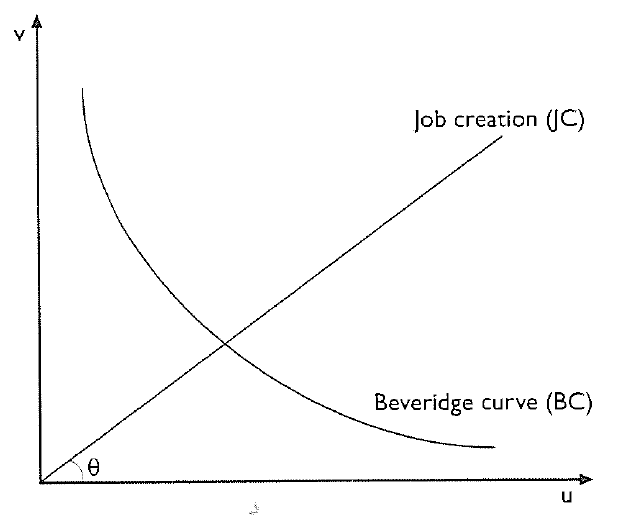
\includegraphics[width=0.4\textwidth]{JC_BC_(v,u).png}%
        \label{fig:a}%
    }%
    \hfill%
    {%
        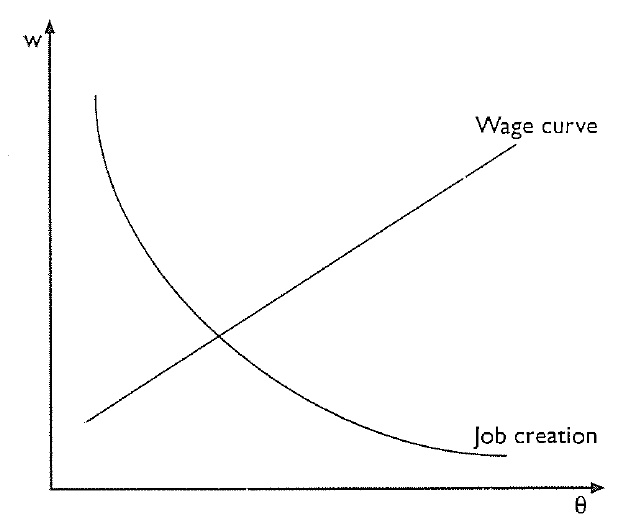
\includegraphics[width=0.4\textwidth]{WC_JC_(w,theta).png}%
        \label{fig:b}%
    }%
    \caption{Equilibrio del mercado laboral. Curva de Beveridge y Curva de Creación laboral}
\end{figure}
\newpage

\hypertarget{tvp-var-2}{%
\section{TVP-VAR}\label{tvp-var-2}}
\begin{itemize}
\tightlist
\item
  Algoritmo, resumen en base a Krüger (\protect\hyperlink{ref-Kruger2015}{2015}):
\end{itemize}
Usando \(B^T= \{B_t\}_{t=1}^T\); \(A^T= \{A_t\}_{t=1}^T\); \(\Sigma^T= \{\Sigma_t\}_{t=1}^T\). Sea \(\theta = [B^T, A^T, V]\) y sea \(V = [Q, S, W]\) una colección de las matrices de varianzas y covarianzas (VCV) de los shocks iid \(\{\nu_t,\zeta_t, \eta_t\}\).
\begin{enumerate}
\def\labelenumi{\arabic{enumi}.}
\tightlist
\item
  Inicializar \(A^T, \Sigma^T, s^T, V\)
\item
  Muestrear \(B^T\) de \(p(B^T|\theta^{-B^T}, \Sigma^T)\), usando el algoritmo de Carter \& Kohn (\protect\hyperlink{ref-KarterKohn1994}{1994}) (CK)
\item
  Muestrear Q de \(p(Q|B^T)\), que se distribuye \(\mathcal{IW}\).
\item
  Muestrear \(A^T\) de \(p(A^T|\theta^{-A^T}, \Sigma^T)\), usando CK
\item
  Muestrear S de \(p(S|\theta^S, \Sigma^T)\)
\item
  Muestrear las variables discretas auxiliares \(s^T\) de \(p(s^T|\Sigma^T, \theta)\) usando el algoritmo de S. Kim, N. Sheppard, \& Chibb (\protect\hyperlink{ref-Kim1998}{1998}).
\item
  Extraer \(\Sigma^T\) de \(p(\Sigma^T|\theta, s^T)\) usando CK
\item
  Muestrear W desde \(p(W|\Sigma^T)\)
\item
  Volver a la etapa 2.
\end{enumerate}


\begin{table}

\caption{\label{tab:priorsTVP}Distribuciones a priori}
\centering
\resizebox{\linewidth}{!}{
\begin{threeparttable}
\begin{tabular}[t]{cccc}
\toprule
Parámetros & Descripción & Familia de priors & Coeficientes\\
\midrule
$B_0$ & Betas iniciales & $\mathcal{N}(\hat{B}_{MCO}, k_B \times\hat{V}(\hat{B}_{MCO}))$ & $k_B = 4$\\
$A_0$ & Covarianza inicial & $\mathcal{N}(\hat{A}_{MCO}, k_A \times \hat{V}(\hat{A}_{MCO}))$ & $k_A = 4$\\
$log \space \sigma_0$ & log volatilidad inivial & $\mathcal{N}(log \space \sigma_{MCO}, k_{\sigma} \times \mathbb{I}_n$ & $k_{\sigma} = 1$\\
$Q$ & $VCV$ de shocks en $B_t$ & $\mathcal{IW}(k^2_Q \times pQ \times \hat{V}(\hat{B}_{MCO}, \space pQ)$ & $k_Q = 0.01, \ pQ = 40$\\
$W$ & $VCV$ de shocks en $log\space \sigma_t$ & $\mathcal{IW}(k^2_W \times pW \times \mathbb{I}_n, \space pW)$ & $k_W=0.01, pW=n+1$\\
\addlinespace
$S_j,\space j=1,...n-1$ & VCV de shocks en $A_t$ & $\mathcal{IW}(k^2_S\times pS_j\times\hat{V}(\hat{A}_{j,MCO}), pS_j)$ & $k_S = 0.01\space,pS_j=j+1$\\
\bottomrule
\end{tabular}
\begin{tablenotes}
\item \textit{Notas:} 
\item \footnotesize Resúmen con las priors utilizadas en el TVP-VAR por Primiceri (\protect\hyperlink{ref-Primiceri2005}{2005}) siguiendo a Krüger (\protect\hyperlink{ref-Kruger2015}{2015}). $\mathcal{IW}$ y $\mathcal{N}$ refieren a las distribuciones inversa de Wishart y Normal. $\hat{A}_{MCO}\space, \hat{V}(\hat{A}_{MCO})\space,\hat{B}_{MCO}\space, \hat{V}(\hat{B}_{MCO})$ se obtienen entrenando una muestra via mínimos cuadrados ordinarios (MCO).
\end{tablenotes}
\end{threeparttable}}
\end{table}
\newpage

\hypertarget{quiebres-estructurales-2}{%
\section{Quiebres estructurales}\label{quiebres-estructurales-2}}

Se asume regresores no estocásticos que convergen a una matriz finita (Q), y \(\Vert x_i\Vert = O(1)\):
\begin{equation}
\frac{1}{n}\sum_{i=1}^nx_ix_i^T \to Q
\end{equation}\footnote{Si bien son condiciones estrictas que no permiten trabajar con procesos con tendencia o que sean dinámicos, pueden ser levantadas. Por ejemplo Hansen (\protect\hyperlink{ref-Hansen1992}{1992}), plantea trabajar con series I(1), mientras Kramer et al. (\protect\hyperlink{ref-Society1988}{1988}) plantean que los test CUSUM mantienen sus niveles de significancia asintótica en modelos dinámicos.}
Los residuos MCO son \(\hat{u_i} = y_i - x_i^T\hat{\beta}\), la varianza estimada \(\hat{\sigma}^2 = \frac{1}{n-k}\sum_i^n\hat{u}_i^2\).
Los residuos recursivos son:
\begin{equation}
\tilde{u}_i = \frac{y_i-x_i^T\hat{\beta}^{(i-1)}}{\sqrt{1+x_i^T(X^{i-1^T}X^{i-1})^{-1}x_i}} \space\space\space\space\space\space i = k+1, ... n
\end{equation}
Donde \(\hat{\beta}^{i-1}\) denota todas las observaciones hasta la observación \(i-1\), lo mismo para \(X^i\). La varianza estimada es \(\tilde{\sigma}^2 = \frac{1}{n-k}\sum_{i=k+1}^n(\tilde{u}_i-\bar{\tilde{u_i}})^2\).
A continuación detallamos los procesos de fluctuación utilizados:
Los procesos CUSUM contienen la suma acumulada de residuos estandarizados, Brown et al. (\protect\hyperlink{ref-Brown1975}{1975}) escribieron el programa TIMVAR donde recomienda la utilización de los residuos recursivos por sobre la suma acumulada de residuos o residuos al cuadrado:
\begin{equation}
W_n(t) = \frac{1}{\tilde\sigma\sqrt \eta}\sum_{i=k+1}^{k+\lfloor t\eta\rfloor}\tilde u_i \space\space\space\space\space 0 \leq t \leq1
\end{equation}
Con \(\eta = n-k\) es el número de residuos recursivos y \(\lfloor t\eta\rfloor\) la parte entera de \(t\eta\). Bajo la hipótesis nula, el proceso límite, sobre el cual se calculan los límites, del proceso empírico \(W_n(t)\) is un proceso de Wiener o un proceso de movimiento Browniano estándar\footnote{Se mantiene el teorema del límite central funcional $W_n \Rightarrow W$ con $n \to \infty$ donde $\Rightarrow$ refiere a convergencia débil de las medidas de probabilidad asociadas.}. Bajo la hipótesis alternativa si existe un único cambio estructural en \(t_0\) los residuos recursivos van a tener media cero hasta \(t_0\). Y para un \(t \geq t_0\) moverse alejados de su media\footnote{Los test CUSUM mantienen sus propiedades en modelos dinámicos Brown et al. (\protect\hyperlink{ref-Brown1975}{1975}) prueban modelos dinámicos y Kramer et al. (\protect\hyperlink{ref-Society1988}{1988}) prueban (Teorema I) que pese a que los residuos recursivos no son normales ni independientes Ploberger et al. (\protect\hyperlink{ref-Ploberger1989}{1989}) en un modelo dinámico, esto no importa asintóticamente puesto que las propiedades se mantienen}.

Ploberger et al. (\protect\hyperlink{ref-Ploberger1989}{1989}) recomienda la utilización de la suma acumulada de residuos MCO:
\begin{equation}
W_n^0(t) = \frac{1}{\hat{\sigma}\sqrt n}\sum_{i=1}^{\lfloor nt\rfloor}\hat{u_i}\space\space\space\space\space 0 \leq t \leq 1
\end{equation}
Donde el proceso límite es un proceso de puente Browniano estándar \(W^0(t) = W(t) - tW(1)\), en \(t_0\) vale 0 y retorna a 0 en \(t = 1\). Si existiera un cambio estructural (único) el trayecto debería tener un salto en torno a \(t_0\).

Los procesos MOSUM, refieren a la suma móvil de residuos, por tanto, el proceso empírico contiene la suma de un número fijo de residuos en una ventana temporal que se mueve a lo largo de todo el periodo y cuyo largo queda determinado por un parámetro de ancho de banda, \(h \in(0,1)\). Al igual que en el caso anterior tenemos dos casos, recursivo y MCO. Los residuos recursivos MOSUM son:
\begin{align}
M_t(t|h) &= \frac{1}{\tilde\sigma\sqrt n}\sum_{i=k+\lfloor N_{\eta}t\rfloor + 1}^{k + \lfloor N_{\eta}t\rfloor + \lfloor \eta h\rfloor}\tilde{u_i} \space\space\space\space\space 0\leq t\leq1-h \\
&= W_n\frac{\lfloor N_{\eta}t\rfloor+\lfloor\eta h\rfloor}{\eta}-W_n\frac{\lfloor N_{\eta}t\rfloor}{\eta}
\end{align}
Con \(N_{\eta} = (\eta - \lfloor\eta h\rfloor/(1-h)\). Mientras los residuos MCO del proceso MOSUM son:
\begin{align}
M_n^0(t|h) &= \frac{1}{\hat{\sigma}\sqrt n}\sum_{i=\lfloor N_{n}t\rfloor + 1}^{\lfloor N_{n}t \rfloor + \lfloor nh\rfloor}\hat{u_i} \space\space\space\space\space\space 0 \leq t \leq 1-h \\
&= W_n^0\frac{\lfloor N_nt\rfloor + \lfloor nh \rfloor}{n} - \frac{\lfloor N_nt\rfloor}{n}
\end{align}
Donde \(N_n = (n - \lfloor nh\rfloor)/(1-h)\). Si, bajo la hipótesis nula, asumimos sucede un único quiebre estructural en \(t_0\), los trayectos tanto de MOSUM-MCO como MOSUM-recursivo deberían tener un quiebre en torno a \(t_0\).

Los límites o frontera de las fluctuaciones de los procesos empíricos (efp) unidimensionales basados en residuos se hacen con respecto a un límite \(b(t)\) y su contraparte \(-b(t)\), el cual el proceso límite cruza con probabilidad \(\alpha\). Sea cruzando \(b(t)\) o \(-b(t)\) para cualquier momento t se concluye que las fluctuaciones es improbablemente grande y la hipótesis nula puede ser rechaza a un nivel de significación \(\alpha\).

Los límites de los procesos MOSUM son constantes \(b(t) = \lambda\), en el caso del proceso recursivo CUSUM son \(b(t) = \lambda(1 + 2t)\), y para CUSUM MCO es \(b(t) = \lambda\)\footnote{En el caso del proceso MOSUM al ser estacionario el proceso límite, tiene sentido que $b(t) = \lambda$. En el caso de los procesos CUSUM los procesos límite no son estacionarios, el movimiento Browniano y de puente Browniano. La elección de los límites se debe a su solución cerrada para las probabilidades de exceder el límite.}.

Por último, dentro de los procesos de fluctuación empíricos tenemos procesos basados en estimadores. En lugar de definir los procesos de fluctuación de acuerdo a los residuos, se definen en base a los parámetros estimados de los regresores, parámetros poblaciones. Los dos procesos siguientes son k-variados.
La estimación recursiva sigue a Ploberger et al. (\protect\hyperlink{ref-Ploberger1989}{1989}):
\begin{equation}
Y_n(t) = \frac{\sqrt i}{\hat{\sigma}\sqrt n}(X^{(i)^T} X^{i})^{\frac{1}{2}}(\hat{\beta}^{(i)} - \hat{\beta}^{(n)})
\end{equation}
Con \(i = \lfloor k + t(n-k)\rfloor\) y \(t \in [0,1]\). Por último la estimación MCO, denotado procesos de estimaciones móviles (ME) es:
\begin{equation}
Z_n(t|h) = \frac{\sqrt{\lfloor nh\rfloor} }{\hat{\sigma}\sqrt{n}}(X^{(\lfloor nt \rfloor , \lfloor nh\rfloor)^T}X^{(\lfloor nt \rfloor , \lfloor nh\rfloor)})^{\frac{1}{2}}(\hat{\beta}^{(\lfloor nt \rfloor , \lfloor nh\rfloor)}-\hat{\beta}^{(n)}) \space\space\space 0 \leq t \leq 1-h
\end{equation}
En ambos casos el proceso límite es un proceso de puente Browniano k-dimensional.
Bajo la hipótesis alternativa de único quiebre, el estimador recursivo debería tener un pico, mientras el estimador de movimiento debería tener un quiebre en torno al punto \(t_0\).

El límite de los efp en este caso, esta dado por \(\Vert efp_i(t) \Vert\), donde \(\Vert . \Vert\) denota un funcional que es aplicado componente a componente. Se trabaja con los funcionales `máximo' y `rango'. Por tanto, la hipótesis nula es rechazada si \(\Vert efp_i \Vert\) es mayor que una constante \(\lambda\) la cual depende del nivel de confianza escogido, \(\alpha\), para cualquier \(i = 1,...k\).

Por último, se trabaja con dos estadísticos para poner a prueba la hipótesis nula. El estadístico \(S_r\) se utilizada para los procesos basados en residuos, mientras el estadístico \(S_e\) se utiliza para los procesos basados en estimaciones:
\begin{align}
S_r &= \max_t\frac{efp(t)}{f(t)}, \\
S_e &= \max \Vert efp(t) \Vert
\end{align}
Con f(t) dependiendo de la forma del límite, \(b(t) = \lambda f(t)\). De donde provienen los distintos cálculos de los p-valores para cada test puede consultarse la sección A en Zeileis et al. (\protect\hyperlink{ref-Zeileis2002}{2002}).

Los estadísticos F difieren de los test anteriores en que se especifica la hipótesis nula a contrastar, se define una hipótesis alternativa de un quiebre en un momento particular.
\begin{equation}
\beta_i = \begin{cases} 
\beta_A &(1 \leq i \leq i_0) \\
\beta_B &(i_0 < i \leq n)
\end{cases}
\end{equation}
Con \(i_0\) es algún punto en el intervalo \((k, n-k)\). El test original de Chow (\protect\hyperlink{ref-Chow1960}{1960}) necesita que se especifique el momento del quiebre en particular en la hipótesis alternativa, o sea, debe ser conocido. Su planteamiento es realizar dos regresiones, una restringida y otra sin restringir.Se ajustan dos regresiones para cada submuestra definida por \(i_0\) y se rechaza \(H_0\) cuando:

\[
F_{i_0} = \frac{\hat{u}^T\hat{u}-\hat{e}^T\hat{e}} {\hat{e}^T\hat{e}/(n-2k)}
\]
el estadístico sobrepasa cierto nivel de tabla. Donde \(\hat{e}=(\hat{u}_A,\hat{u}_B)\) son los residuos del modelo completo sin restringir. Para examinar la igualdad entre los conjuntos de coeficientes in dos regresiones lineal, se obtienen la suma cuadrado de los residuos asumiendo igualdad (bajo \(H_0\)) y la suma de los cuadrados sin asumir igualdad. El ratio de la diferencia entre las dos sumas y la última suma, ajustado por los correspondientes grados de libertad se distribuye como el estadístico F bajo \(H_0\) Chow (\protect\hyperlink{ref-Chow1960}{1960})\footnote{Los resultados de Chow (\protect\hyperlink{ref-Chow1960}{1960}) se pueden resumir en sus ecuaciones 50 y 51 y, son generalizables al caso de más de dos regresiones.}. Específicamente, \(F_{i_0} \sim \chi^2_k\) y \(F_{i_0}/k \sim \chi^2_{k, n-2k}\). La desventaja del planteamiento de Chow, es que el punto de quiebre debe ser conocido a priori, sin embargo, dicha limitación puede ser levantada. Es posible plantear un test F para todos los potenciales puntos de quiebre en casi toda la muestra o en un intervalo de la misma, cumpliendo que \(k < \underline i \leq \overline i \leq n-k\). Rechazando \(H_0\) si cualquier estadístico, \(F_i\) sobrepasa los valores de tabla. Por ejemplo, si pensamos que existe una cambio estructural entre 1990 y 2010 que genero una alteración en los parámetros del modelo, podemos definir dicho intervalo y correr test F de forma iterativa, buscando algún quiebre en cualquiera de dichos años. El beneficio es mayúsculo, no necesitamos asumir un punto y obtenemos donde se genera el quiebre. Sin embargo, seguimos obteniendo solamente un quiebre, pero dicho problema se puede resolver utilizando un algoritmo que minimice una función objetivo y basado en el principio de optimalidad de Bellman encuentre una partición óptima Bai \& Perron (\protect\hyperlink{ref-BaiPerron1998}{1998}), Bai \& Perron (\protect\hyperlink{ref-BaiPerron2003}{2003}), Zeileis et al. (\protect\hyperlink{ref-Zeileis2010}{2010}).

Al igual que los efp, es posible plantear límites para el estadístico F. Asumiendo \(H_0\), los límites se pueden calcular de tal forma que la probabilidad asintótica de alguna forma de agregación de los distintos estadísticos F calculados sobre los intervalos considerados \(\underline i \leq i \leq \bar{i}\), superen dicho umbral con una significación \(\alpha\). Andrews (\protect\hyperlink{ref-Andrews1993}{1993}), Andrews \& Ploberger (\protect\hyperlink{ref-Andrews1994}{1994}) plantean tres funcionales a utilizar: el supremo, la media o exponencial, con lo cual plantean tres opciones para poner a prueba la hipótesis nula:
\begin{align}
supF &= \sup_{\underline i \leq i \leq \bar{i}} F_i \\
aveF &= \frac{1}{\bar{i} - \underline i + 1}\sum_{i = \underline i}^{\bar{i}}F_i \\
expF &= log \left( \frac{1}{\bar{i}-\underline i + 1}\sum_{i = \underline i}^{\bar{i}}exp(0.5\times F_i) \right)
\end{align}
Si sucede que el funcional de los estadísticos F cruza dicho umbral, entonces existe evidencia de un cambio estructural con una significación \(\alpha\). Sin embargo, el problema con los test F, es que nos dan información de un solo quiebre en los parámetros, cuando podrían existir varios. Bai \& Perron (\protect\hyperlink{ref-BaiPerron1998}{1998}) plantean el problema, solución teórica y propiedades dentro de un marco general que engloba a un modelo estructural completo y parcial\footnote{La diferencia entre un modelo estructural completo es que todos los parámetros pueden tener quiebres en la muestra, mientras un modelo estructural parcial permite a un subconjunto de los parámetros tener quiebres, mientras el resto son estimados con la muestra completa asumiéndolos invariables}, Bai \& Perron (\protect\hyperlink{ref-BaiPerron2003}{2003}) implementan dicha solución utilizando la ecuación de Bellman de programación dinámica y la función objetivo de MCO, mientras Zeileis et al. (\protect\hyperlink{ref-Zeileis2010}{2010}) amplía la solución para cuasi-máxima verosimilitud y una función objetivo de minimización de la log-verosimilitud negativa.

Siguiendo a Bai \& Perron (\protect\hyperlink{ref-BaiPerron2003}{2003}), se considera el siguiente modelo matricial con m quiebres y m+1 regímenes\footnote{Si \(p = 0\) estamos frente a un modelo estructural puro, donde todos los coeficientes pueden variar. La varianza de \(u_i\) no es necesario que sea constante, de hecho puede cambiar en el mismo momento en que cambian los parámetros y mejorar la precisión de los quiebres en los estimadores, sin embargo, Bai \& Perron (\protect\hyperlink{ref-BaiPerron2003}{2003}) lo tratan como un parámetro molesto `nuisance parameter'.}
\begin{equation}
Y = X\beta + \bar{Z}\delta + U
\end{equation}
donde \(Y = (y_1, ...y_T)'\), \(X = (x1, ... x_T)'\), \(U = (u_1, ...u_T)'\), \(\delta = (\delta_1',...\delta_{m+1}')'\) y \(\bar{Z}\) es la matriz diagonal con particiones de \(Z\) en \((T_1, ...T_m)\), es decir, \(\bar{Z} = diag(Z_1, ... Z_{m+1})\) con \(Z_i = (z_{T_{i-1}}, ..., z_{T_{i}})'\). Los puntos de quiebre \((T_1, ...T_m)\), son tratados como desconocidos. Se busca estimar los coeficientes conjuntamente con los quiebres.

Los valores de los parámetros verdaderos se denotan con 0. Es decir, \(\delta^0 = (\delta_{1}'^0,...\delta_{m+1}'^0)'\) y \((T_1^0, ...T_m^0)\) denotan los verdaderos valores de los parámetros y de los quiebres. La matriz \(\bar{Z}^0\) es la que particiona diagonalmente \(Z\) en \((T_1^0, ...T_m^0)\). Por lo cual, el proceso generador de datos se asume:
\begin{equation}
Y = X\beta^0 + \bar{Z}^0\delta^0 + U
\end{equation}
Usando el método de estimación es MCO. Para cada m-partición \((T_1, ...T_m)\) los estimadores MCO asociados de \(\beta\) y \(\delta_j\) son obtenidos mediante la minimización de la suma cuadrado de los residuos (RSS):

\[
(Y - X\beta - \bar{Z}\delta)'(Y - X\beta - \bar{Z}\delta) = \sum_{i=1}^{m+1}\sum_{t = T_{i-1}+1}^{T_i}[y_t-x_t'\beta-z_t'\delta_i]^2
\]
Siendo \(\hat{\beta}(\{T_j\})\) y \(\hat{\delta}(\{T_j\})\) las estimaciones en cada m-partición \((T_1, .. T_m)\) denotada \(\{T_j\}\). Substituyendo estos últimos en la función objetivo y denotando RSS como \(S_T(T_1, ... T_m)\) los puntos de quiebre estimados \((\hat{T}_1, ..., \hat{T}_m)\) son tal que:

\[
(\hat{T}_1, ..., \hat{T}_m) = arg\min_{T_1,...T_m}S_T(T_1, ... T_m)
\]
La minimización se realiza sobre todas las particiones \((T_1, ...T_m)\) de forma tal que \(T_i - T_{i-1} \geq q\). Por lo tanto, los estimadores de punto de quiebre son minimizadores globales de la función objetivo\footnote{Notar que se puede elegir cualquier función objetivo a minimizar}. Las estimaciones de los parámetros de regresión, son las estimaciones asociadas con cada m-partición \(\{{\hat{T}_j}\}\), es decir, \(\hat{\beta} = \hat{\beta}({\hat{\{T_j\}}})\), \(\hat{\delta} = \hat{\delta}({\hat{\{T_j\}}})\). Ya que los puntos de quiebre son parámetros discretos y pueden tomar únicamente un número finito de valores, se pueden estimar mediante una grilla de valores (grid search), sin embargo dicho algoritmo tiene complejidad \(O(T^m)\).

Para poder computar dichos estimadores, Bai \& Perron (\protect\hyperlink{ref-BaiPerron2003}{2003}) utilizan el principio de optimalidad de Bellman o principio de programación dinámica cuya complejidad es \(O(T^2)\) independientemente de la cantidad particiones que se realicen. Una vez que los RSS de los segmentos relevantes\footnote{Los segmentos relevantes refieren a los segmentos plausibles de ser estimados, ver sección 3.1 Bai \& Perron (\protect\hyperlink{ref-BaiPerron2003}{2003})} han sido calculados, se utiliza el enfoque de programación dinámica para evaluar que partición logra una minimización global sobre RSS.

Sea \(RSS(\{T_{r,n}\})\) la suma de cuadrados de residuos asociada con la partición optima conteniendo \(r\) quiebres usando las primeras n observaciones. La partición óptima resuelve el siguiente problema recursivo:

\[
RSS(\{T_{m,T}\}) = \min_{mh\leq j\leq T-h}[RSS(\{T_{m-1,j}\}) + RSS(\{j+1, T\})]
\]

Se evalúa primero, el primer quiebre óptimo para todas las submuestras desde \(h\) hasta \(T-mh\). Se guardan un conjunto de \(T-(m+1)h+1\) particiones óptimas y sus RSS, donde cada partición corresponde a una submuestra terminando en \(2h\) hasta \(T-(m-1)h\).
Segundo, se buscan las particiones óptimas con dos quiebres, las cuales terminan en el periodo \(3h\) hasta \(T-(m-2)h\). Para cada uno de estas posibles fechas de término, se busca en que partición de un quiebre guardada previamente puede ser insertada para obtener un RSS mínimo. Se devuelve un conjunto de \(T-(m+1)h+1\) con dos quiebres óptimos. El algoritmo continua de forma secuencial hasta que el conjunto \(T-(m+1)h+1\) de \((m-1)\) particiones óptimas se obtiene con finalización desde \((m-1)h\) hasta \(T-2h\). Por último, se busca cual de esas \((m-1)\) particiones óptimas genera un mínimo global en RSS cuando se combina con un segmento adicional.

Por último, Zeileis et al. (\protect\hyperlink{ref-Zeileis2010}{2010}) extiende el trabajo de Bai \& Perron (\protect\hyperlink{ref-BaiPerron2003}{2003}), para trabajar con modelos de tipo de cambio, como Frankel \& Wei (\protect\hyperlink{ref-Frankel1994}{1994}) en los cuales la varianza del error \(\sigma^2\)es de crucial interés. Esto lleva a la inclusión del error de la varianza como un regresor adicional en vez de un parámetro molesto y, la estimación del modelo por máxima verosimilitud o cuasi-máxima verosimilitud, en lugar de MCO. La inclusión de \(\sigma^2\) no debe ser visto como relevante solo para modelos de tipo cambio, como nota Bai \& Perron (\protect\hyperlink{ref-BaiPerron2003}{2003}) su inclusión puede mejorar la estimación de los quiebres estructurales.

El modelo planteado es cuasi-normal y tiene densidad:
\[
f(y|x,\beta, \sigma^2) = \phi((y-x^T\beta)/\sigma)/\sigma
\]
Donde \(\phi(.)\) es la función de densidad de una normal estándar. Con \(\theta = (\beta^T, \sigma^2)^T\) de largo \(k = c +2\), siendo c la cantidad de regresores, más intercepto y varianza.

El algoritmo para encontrar quiebres es exactamente el mismo que Bai \& Perron (\protect\hyperlink{ref-BaiPerron2003}{2003}), con la diferencia que en vez de usar estimaciones MCO se usan estimaciones QML y la función objetivo \(RSS\) se cambia por la log-verosimilitud negativa \(-logf(y_i|x_i, \theta)\)

\newpage

\hypertarget{datos}{%
\section{Datos}\label{datos}}
\begin{figure}
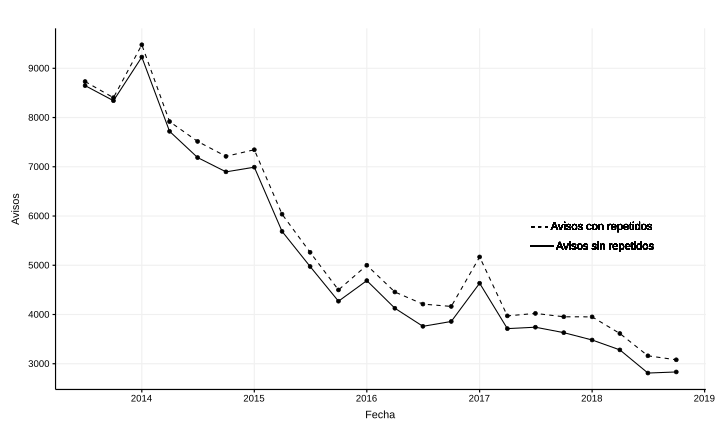
\includegraphics[width=\maxwidth]{tesis_files/figure-latex/ga13-18-comparacion-1.pdf}
\caption{Avisos diario El País}\label{fig:ga13-18-comparacion}\textsc{}

\footnotesize\textsc{Notas} -- Series de avisos laborales de \textit{Gallito} entre 2013 y 2018. Las series refieren a los avisos publicados filtrados por link (id) de aviso y a la cantidad de publicaciones sin filtrar. Se observa una diferencia de nivel relativamente estable.

\textsc{Fuentes} -- Avisos publicados en el portal web \textit{Gallito}. Datos confidenciales facilitados por diario El País. Procesamiento propio.
\end{figure}


\begin{figure}
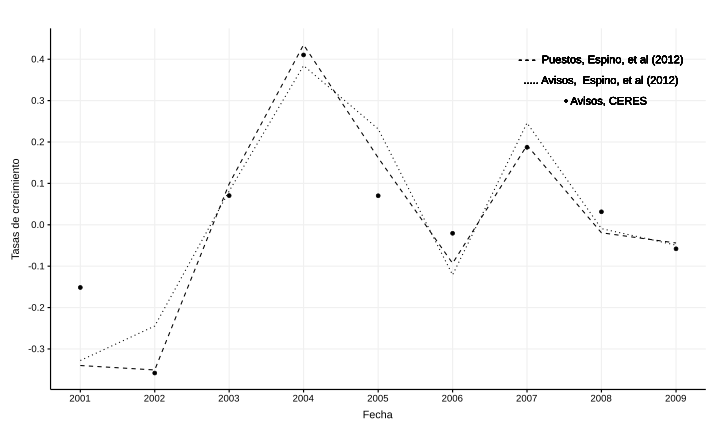
\includegraphics[width=\maxwidth]{tesis_files/figure-latex/iecon-ceres-1.pdf}
\caption{Comparación tasas de crecimiento}\label{fig:iecon-ceres}\textsc{}

\footnotesize\textsc{Notas} -- Tasas de crecimiento de series de vacantes laborales anualizadas entre los años 2000 a 2009 correspondientes a Espino et al. (\protect\hyperlink{ref-Alma2011}{2011}) y CERES (\protect\hyperlink{ref-Ceres2012}{2012}). La línea punteada corresponde a los avisos recolectados en Espino et al. (\protect\hyperlink{ref-Alma2011}{2011}) mientras la línea cortada corresponde a los puestos laborales. Los puntos corresponden a los datos transformados a partir de CERES (\protect\hyperlink{ref-Ceres2012}{2012}). Se observa una elevada correlación lineal entre las tasas de crecimiento de avisos en el orden del 90\% que corrobora que el ICDL esta construido a partir de publicaciones laborales de \textit{Gallito}.

\textsc{Fuentes} -- Los datos de Espino et al. (\protect\hyperlink{ref-Alma2011}{2011}) han sido facilitado por los autores y la información de CERES (\protect\hyperlink{ref-Ceres2012}{2012}) ha sido facilitada por CERES. Las series son de elaboración propia.
\end{figure}
\begin{figure}
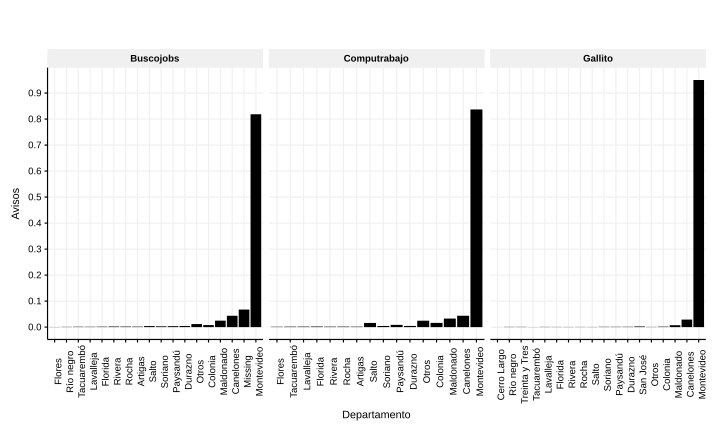
\includegraphics[width=\maxwidth]{tesis_files/figure-latex/avisos-dpto-1.pdf}
\caption{Avisos recolectados mediante scraping}\label{fig:avisos-dpto}\textsc{}

\footnotesize\textsc{Notas} -- Proporción de avisos laborales publicados en cada portal web laboral para cada departamento de Uruguay. Entre el 80\%-95\% de los avisos laborales corresponde al departamento de Montevideo, evidenciando que existe un sesgo pequeño de avisos laborales de otros departamentos.

\textsc{Fuentes} -- Datos recolectados mediante scraping web de los portales laborales \textit{Buscojobs}, \textit{Computrabajo}, \textit{Gallito} durante el último trimestre de 2018 y todo 2019.
\end{figure}
\begin{figure}
\includegraphics[width=\maxwidth]{tesis_files/figure-latex/gallito-13-18-1.pdf}
\caption{Avisos laborales \textit{Gallito} por nivel jerárquico}\label{fig:gallito-13-18}\textsc{}

\footnotesize\textsc{Notas} -- Proporción de avisos laborales en \textit{Gallito} entre 2013-2018 por nivel jerárquico. Cerca de un 40\% de los avisos corresponden a auxiliares, un 15\% a técnico o especialista, un 10\% a peón y cerca de un 2\% a puestos de gerente.

\textsc{Fuentes} -- Datos del portal laboral \textit{Gallito}, facilitados por el diario El País. Procesamiento propio.
\end{figure}
\newpage

\hypertarget{resultados}{%
\section{Resultados}\label{resultados}}

\hypertarget{uxedndice-de-vacantes-buscojobs-y-computrabajo}{%
\subsection{Índice de vacantes, Buscojobs y Computrabajo}\label{uxedndice-de-vacantes-buscojobs-y-computrabajo}}
\begin{figure}
\includegraphics[width=\maxwidth]{tesis_files/figure-latex/serie-buscojobs-1.pdf}
\caption{Serie trimestral \textit{Buscojobs}}\label{fig:serie-buscojobs}\textsc{}

\footnotesize\textsc{Notas} -- Serie trimestral de avisos laborales publicados en el portal \textit{Buscojobs}, construcción y elaboración propia

\textsc{Fuentes} -- Los datos fueron obtenidos a través del portal \textit{Waybackmachine}, scraping de \textit{Buscojobs} y finalmente imputando los valores faltantes.
\end{figure}
\begin{figure}
\includegraphics[width=\maxwidth]{tesis_files/figure-latex/serie-computrabajo-1.pdf}
\caption{Serie trimestral \textit{Computrabajo}}\label{fig:serie-computrabajo}\textsc{}

\footnotesize\textsc{Notas} -- Serie trimestral de avisos laborales publicados en el portal \textit{Computrabajo}, construcción y elaboración propia.

\textsc{Fuentes} -- Los datos fueron obtenidos a través del portal \textit{Waybackmachine}, scraping de \textit{Computrabajo} y finalmente imputando los valores faltantes.
\end{figure}
\hypertarget{caracterizaciuxf3n-de-las-series}{%
\subsection{Caracterización de las series}\label{caracterizaciuxf3n-de-las-series}}

Se han realizado distintos test de raíz unitaria regular (RU) y raíz unitaria estacional sobre la serie de vacantes, tasa de desempleo y sobre las series que componen el índice de vacantes. En el Cuadro \ref{tab:test-ru-trim} del anexo, todas las series trimestrales utilizadas en el análisis son PGD que requieren una diferencia regular para ser estacionarios, a excepción del portal web \emph{Buscojobs}\footnote{Cuando se realizan los mismos test con \emph{Buscojobs} con frecuencia mensual, el test ADF y PP siguen planteando que el PGD no necesita diferencias regulares para ser estacionario. El test KPSS da como resultado la necesidad de una diferencia para que el proceso sea estacionario, ver Cuadro \ref{tab:test-ru-mensual}}.

Posteriormente analizamos si la tasa de desempleo y el índice de vacantes están cointegrados. Dado que las series se correlacionan negativamente se plantea la relación entre las vacantes y la inversa de la tasa de desempleo. En todos los casos no se rechaza la hipótesis nula de no cointegración (ver anexo).







\begin{table}

\caption{\label{tab:test-ru-trim}Test de raíces unitarias series trimestrales}
\centering
\resizebox{\linewidth}{!}{
\begin{threeparttable}
\begin{tabular}[t]{ccccc}
\toprule
Serie & Test RU regular & Diferencias & Test RU estacional & Diferencias\\
\midrule
\textit{Gallito} 80-19 & ADF-KPSS-PP & 1 & HEGY-OCSB-CH & 0\\
\textit{Urr-Mol} 80-01 & ADF-KPSS-PP & 1 & HEGY-OCSB-CH & 1-0-0\\
\textit{Computrabajo} 03-19 & ADF-KPSS-PP & 1 & HEGY-OCSB-CH & 1-0-0\\
\textit{Buscojobs} & ADF-KPSS-PP & 0 & HEGY-OCSB-CH & 1-0-0\\
Serie Final & ADF-KPSS-PP & 1 & HEGY-OCSB-CH & 0\\
\addlinespace
PEA & ADF-KPSS-PP & 1 & HEGY-OCSB-CH & 0\\
Tasa Desempleo & ADF-KPSS-PP & 1 & HEGY-OCSB-CH & 0\\
PIB & ADF-KPSS-PP & 1 & HEGY-OCSB-CH & 0\\
Índice de Vacantes & ADF-KPSS-PP & 1 & HEGY-OCSB-CH & 0\\
\bottomrule
\end{tabular}
\begin{tablenotes}
\item \textit{Notas:} 
\item \footnotesize Test de raíces unitarias regulares y estacionales. Los test de raíces unitarias regulares son: ADF es el test de Dickey-Fuller aumentado Dickey \& Fuller (\protect\hyperlink{ref-DickeyFuller1979}{1979}), el test KPSS corresponde a Kwiatkowski, Phillips, Schmidt, \& Shin (\protect\hyperlink{ref-KPSS1992}{1992}) y el test PP refiere a Phillips \& Perron (\protect\hyperlink{ref-PhillipsPerron1988}{1988}). En la medida que las hipótesis nulas en los tres test no son iguales, la columna \textit{Diferencias} refiere a la cantidad de diferencias regulares necesarias para que el proceso estócastico sea estacionario en covarianza. En todos los casos a excepción de \textit{Buscojobs} los test coinciden en que es necesaria una diferencia regular. Los test de raíces unitarias estacionales son: HEGY corresponde a Hylleberg, Engle, Granger, \& Yoo (\protect\hyperlink{ref-hegy1990}{1990}), OCSB a Osborn, Chui, Smith, \& Birchenhall (\protect\hyperlink{ref-Osborn1988}{1988}) y CH al test de Canova (\protect\hyperlink{ref-Canova1995}{2014}). A excepción de las series de Urr-mol (Urrestarazu-Molina), \textit{Computrabajo} y \textit{Buscojobs} donde los test difieren en sus conclusiones, los test coinciden en que no es necesaria una diferencia estacional para el resto de las series.
\end{tablenotes}
\end{threeparttable}}
\end{table}
El Cuadro \ref{tab:test-ru-trim} columna 2 muestra los resultados de la aplicación de los test Dickey Fuller Aumentado (ADF) (Dickey \& Fuller, \protect\hyperlink{ref-DickeyFuller1979}{1979}), Kwiatkowski--Phillips--Schmidt--Shin (KPSS) (Kwiatkowski et al., \protect\hyperlink{ref-KPSS1992}{1992}) y Phillips-Perron (PP) (Phillips \& Perron, \protect\hyperlink{ref-PhillipsPerron1988}{1988}). El test ADF y PP usan la hipótesis nula que la serie tiene una raíz unitaria versus una hipótesis alternativa de una raíz estacionaria. En el test KPSS la hipótesis nula es que la serie tiene una raíz estacionaria contra una hipótesis alternativa de raíz unitaria. La columna diferencias refiere a la cantidad de diferencias regulares necesarias para que la realización del proceso estócastico se vuelva estacionario. El resultado es que la serie de vacantes es un proceso integrado I(1), al igual que dos de las tres series que la componen, la serie de avisos de \emph{Gallito} (años 80 a 2019) y la serie de \emph{Computrabajo} (2003 a 2019), mientras \emph{Buscojobs} resulta ser I(0). Tanto el PIB como la tasa de desempleo, resultan procesos integrados de orden uno.

La columna test estacional, muestra los test de raíz unitaria estacional realizados. El test de Hylleberg et al. (\protect\hyperlink{ref-hegy1990}{1990}) (HEGY) pone aprueba la hipótesis nula de que las raíces del polinomio autoregresivo caen dentro del circulo unitario versus la alternativa que caen fuera. El test Osborn et al. (\protect\hyperlink{ref-Osborn1988}{1988}) (OCSB) utiliza la hipótesis nula de raíz unitaria estacional versus la alternativa de estacionariedad. Mientras el test Canova (\protect\hyperlink{ref-Canova1995}{2014}) (CH) plantea la hipótesis nula de la no existencia de raíz unitaria en las frecuencias estacionales versus la alternativa de raíz unitaria en una frecuencia estacional o en un conjunto de frecuencias estacionales. La última columna de la tabla refiere a la cantidad de diferencias estacionales necesarias para que el proceso se vuelva estacionario, los tres test llevan a las mismas conclusiones tanto para el PIB, tasa de desempleo e índice de vacantes, no son necesarias diferencias estacionales. Sin embargo, en el caso de la serie de \emph{Buscojobs} y \emph{Computraajo} los resultados difieren, para ambas el test HEGY plantea la existencia de raíz unitaria en frecuencias estacional mientras los test OCSB y CH la descartan.

Por último el Cuadro \ref{tab:test-ru-mensual} realiza lo mismos test pero con un subconjunto de series de frecuencia mensual. Las series de \emph{Gallito} y \emph{Computrabajo}, muestran resultados sin ambigüedades, son procesos I(1) mientras \emph{Buscojobs} es un proceso I(1) para KPSS pero I(0) para ADF y PP, notar que cuando la serie es trimestralizada los tres test coinciden. Los test de raíz unitaria estacional plantean que no es necesario realizar diferencias estacionales tanto para \emph{Computrabajo} como \emph{Buscojobs}, por el contrario, la serie de \emph{Gallito} según HEGY y CH necesita una diferencia estacional, no así para OCSB. Dicho resultado difiere cuando la serie es trimestralizada, en donde los tres test coinciden en la no existencia de raíz unitaria estacional.
\begin{table}

\caption{\label{tab:test-ru-mensual}Test de raíces unitarias series mensuales}
\centering
\resizebox{\linewidth}{!}{
\begin{threeparttable}
\begin{tabular}[t]{ccccc}
\toprule
Serie & Test RU regular & Diferencias & Test RU estacional & Diferencias\\
\midrule
Gallito 13-19 & ADF-KPSS-PP & 1 & HEGY-OCSB-CH & 1-0-1\\
Computrabajo 03-19 & ADF-KPSS-PP & 1 & HEGY-OCSB-CH & 0-0-0\\
Buscojobs 07-19 & ADF-KPSS-PP & 0-1-0 & HEGY-OCSB-CH & 0-0-0\\
\bottomrule
\end{tabular}
\begin{tablenotes}
\item \textit{Notas:} 
\item \footnotesize Test de raíces unitarias regulares y estacionales. Los test de raíces unitarias regulares son: ADF es el test de Dickey-Fuller aumentado Dickey \& Fuller (\protect\hyperlink{ref-DickeyFuller1979}{1979}), el test KPSS corresponde a Kwiatkowski, Phillips, Schmidt, \& Shin (\protect\hyperlink{ref-KPSS1992}{1992}) y el test PP refiere a Phillips \& Perron (\protect\hyperlink{ref-PhillipsPerron1988}{1988}). En la medida que las hipótesis nulas en los tres test no son iguales, la columna \textit{Diferencias} refiere a la cantidad de diferencias regulares necesarias para que el proceso estócastico sea estacionario en covarianza. En todos los casos a excepción de \textit{Buscojobs} los test coinciden en que es necesaria una diferencia regular. Los test de raíces unitarias estacionales son: HEGY corresponde a Hylleberg, Engle, Granger, \& Yoo (\protect\hyperlink{ref-hegy1990}{1990}), OCSB a Osborn, Chui, Smith, \& Birchenhall (\protect\hyperlink{ref-Osborn1988}{1988}) y CH al test de Canova (\protect\hyperlink{ref-Canova1995}{2014}). A excepción de la serie de \textit{Gallito} donde los test difieren en sus conclusiones, los test coinciden en que no es necesaria una diferencia estacional para el resto de las series.
\end{tablenotes}
\end{threeparttable}}
\end{table}
\hypertarget{cointegraciuxf3n}{%
\subsection{Cointegración}\label{cointegraciuxf3n}}

Dada la correlación negativa entre vacantes y desempleo, y el orden de integración igual a 1 no es esperable que exista una relación de largo plazo entre las series, cuando un proceso aumenta el otra disminuye, por lo cual los residuos de una regresión lineal entre ambas serán diferentes de un proceso I(0), lo que si debería pasar es que la velocidad de las series, es decir, sus tasas de crecimiento tengan una relación estable.
se lleva a cabo el test de cointegración de Phillips-Ouliaris entre el índice de vacantes y la tasa de desempleo. Dado que el test no es invariante a la formulación de la ecuación de regresión, se realizan dos test utilizando como variable dependiente al índice de vacantes y luego la tasa de desempleo. En ambos casos, no se rechaza la hipótesis nula de no cointegración al 10\%.
Una vez que se toman logaritmos y se diferencian las series, se rechaza la hipótesis nula de no cointegración al 1\% indicando que las tasas de crecimiento del índice de vacantes laborales y la tasa de desempleo están cointegradas. El resultado se mantiene para la aceleración de las series. Por lo tanto, tanto la velocidad como la aceleración de las vacantes laborales y la tasa de desempleo muestran una relación estable en el largo plazo, lo cual era esperable.

Se realiza el mismo procedimiento pero esta vez probando la hipótesis nula de no cointegración entre PIB y vacantes, posteriormente PIB y desempleo. En ambos casos no se rechaza la hipótesis nula de no cointegración al 10\%. Realizamos el mismo procedimiento con la tasa de crecimiento del PIB y vacantes, luego con la tasa de crecimiento del PIB y tasa de desempleo. En ambos se rechaza la hipótesis nula de no cointegración al 1\%, el procedimiento devuelve el mismo resultado si se usa la tasa de variación de vacantes o desempleo.

Finalmente siguiendo a Johansen (\protect\hyperlink{ref-Johansen1991}{1991}), se plantean los test de traza y valor propio para las series del PIB, tasa de desempleo e índice de vacantes, el resultado es que no se rechaza la hipótesis nula de no cointegración al 10\%\footnote{Sin embargo, si se utiliza la tasa de crecimiento del PIB, se rechaza la hipótesis nula de no cointegración al 1\%, y no se rechaza que exista 1 relación de cointegración. Finalmente, si se utilizan solamente las tasas de crecimiento de las variables, no se rechaza la existencia de 3 relaciones de cointegración. Dichos resultados son robustos frente a la especificación de los vectores de cointegración con tendencia, constante o ninguna. Es decir, existe una relación estable de largo plazo entre las tasas de crecimiento del PIB, índice de vacantes y tasa de desempleo.}.

\hypertarget{efpAnexo}{%
\subsection{Procesos de fluctuación empíricos}\label{efpAnexo}}
\begin{figure}
\includegraphics[width=\maxwidth]{tesis_files/figure-latex/testCUSUM-1.pdf}
\caption{Test CUSUM}\label{fig:testCUSUM}\textsc{}

\footnotesize\textsc{Notas} -- Procesos de fluctuación empíricos bajo el marco de test de fluctuación generalizados. Se visualizan el proceso empírico y su frontera (con color rojo). El proceso supera la frontera indicando la posible existencia de un quiebre estructural en la media incondicional.

\textsc{Fuentes} -- Los datos utilizados son el índice de vacantes de construcción propia y la tasa de desempleo generada por el INE.
\end{figure}
\begin{figure}
\includegraphics[width=\maxwidth]{tesis_files/figure-latex/TestRecursivos-1.pdf}
\caption{Test score}\label{fig:TestRecursivos}\textsc{}

\footnotesize\textsc{Notas} -- Procesos de fluctuación empíricos bajo el marco de test de fluctuación generalizados. Se visualizan el proceso empírico y su frontera (con color rojo). El proceso supera la frontera indicando la posible existencia de un quiebre estructural en la media incondicional. Adicionalmente se gráfica el proceso empírico y frontera para la varianza, y la misma cruza los límites indicado posibles quiebres.

\textsc{Fuentes} -- Los datos utilizados son el índice de vacantes de construcción propia y la tasa de desempleo generada por el INE.
\end{figure}
\begin{figure}
\includegraphics[width=\maxwidth]{tesis_files/figure-latex/TestRecursivos-2.pdf}
\caption{Test score}\label{fig:TestRecursivos}\textsc{}

\footnotesize\textsc{Notas} -- Procesos de fluctuación empíricos bajo el marco de test de fluctuación generalizados. Se visualizan el proceso empírico y su frontera (con color rojo). El proceso supera la frontera indicando la posible existencia de un quiebre estructural en la media incondicional. Adicionalmente se gráfica el proceso empírico y frontera para la varianza, y la misma cruza los límites indicado posibles quiebres.

\textsc{Fuentes} -- Los datos utilizados son el índice de vacantes de construcción propia y la tasa de desempleo generada por el INE.
\end{figure}
\begin{figure}
\includegraphics[width=\maxwidth]{tesis_files/figure-latex/testMOSUM-1.pdf}
\caption{Test MOSUM}\label{fig:testMOSUM}\textsc{}

\footnotesize\textsc{Notas} -- Procesos de fluctuación empíricos bajo el marco de test de fluctuación generalizados. Se visualizan el proceso empírico y su frontera (con color rojo). El proceso supera la frontera indicando la posible existencia de un quiebre estructural en la media incondicional.

\textsc{Fuentes} -- Los datos utilizados son el índice de vacantes de construcción propia y la tasa de desempleo generada por el INE.
\end{figure}
\begin{figure}
\includegraphics[width=\maxwidth]{tesis_files/figure-latex/testME-1.pdf}
\caption{test ME}\label{fig:testME}\textsc{}

\footnotesize\textsc{Notas} -- Procesos de fluctuación empíricos bajo el marco de test de fluctuación generalizados. Se visualizan el proceso empírico y su frontera (con color rojo). El proceso supera la frontera indicando la posible existencia de un quiebre estructural en la media incondicional.

\textsc{Fuentes} -- Los datos utilizados son el índice de vacantes de construcción propia y la tasa de desempleo generada por el INE.
\end{figure}
\begin{figure}
\includegraphics[width=\maxwidth]{tesis_files/figure-latex/testME-2.pdf}
\caption{test ME}\label{fig:testME}\textsc{}

\footnotesize\textsc{Notas} -- Procesos de fluctuación empíricos bajo el marco de test de fluctuación generalizados. Se visualizan el proceso empírico y su frontera (con color rojo). El proceso supera la frontera indicando la posible existencia de un quiebre estructural en la media incondicional.

\textsc{Fuentes} -- Los datos utilizados son el índice de vacantes de construcción propia y la tasa de desempleo generada por el INE.
\end{figure}
\hypertarget{test-de-quiebres-estructurales}{%
\subsection{Test de quiebres estructurales}\label{test-de-quiebres-estructurales}}


\begin{table}[!h]

\caption{\label{tab:quiebres}Test de quiebres estructurales}
\centering
\begin{threeparttable}
\begin{tabular}[t]{>{\centering\arraybackslash}p{5cm}>{\centering\arraybackslash}p{2.5cm}>{\centering\arraybackslash}p{2.5cm}>{\centering\arraybackslash}p{2.5cm}}
\toprule
Test & Estadístico & p-valor & Significación\\
\midrule
Rec-CUSUM & 5.36 & 0.00 & ***\\
OLS-CUSUM & 4.69 & 0.00 & ***\\
Score-CUSUM & 3.94 & 0.00 & ***\\
Rec-CUSUM(d) & 1.96 & 0.00 & ***\\
OLS-CUSUM(d) & 1.23 & 0.10 & ***\\
\addlinespace
Score-CUSUM(d) & 1.58 & 0.05 & .\\
Rec-MOSUM & 4.57 & 0.01 & *\\
OLS-MOSUM & 3.22 & 0.01 & *\\
Score-MOSUM & 3.33 & 0.01 & *\\
fluctuation & 4.80 & 0.00 & ***\\
\addlinespace
ME & 19.64 & 0.01 & *\\
\bottomrule
\end{tabular}
\begin{tablenotes}
\small
\item \textit{Notas:} 
\item \footnotesize Test de quiebres estructurales de fluctuación generalizada, basados en residuos y estimadores. La columna \textit{Test} presenta los test realizados siguiendo la nomenclatura usada por Zeileis et al. (\protect\hyperlink{ref-Zeileis2002}{2002}). \textit{Estadístico} muestra el valor de los estadísticos, \textit{p-valor} refiere a dicho valor para cada prueba. \textit{Significación} muestra los niveles de significación donde . quiere decir no significativo al 5\% pero si al 10\%. Un * es estadísticamente significativo al 5\%, ** es significativo al 1\% mientras *** es significativo al 0.1\%. Todos los test son estadísticamente significativos al 5\% a excepción del test Score-CUSUM(d).
\end{tablenotes}
\end{threeparttable}
\end{table}


\begin{table}[!h]

\caption{\label{tab:ftest}Test de estadístico F}
\centering
\begin{threeparttable}
\begin{tabular}[t]{>{\centering\arraybackslash}p{3cm}>{\centering\arraybackslash}p{3cm}>{\centering\arraybackslash}p{3cm}>{\centering\arraybackslash}p{3cm}}
\toprule
Test & Estadístico & p-valor & Significación\\
\midrule
expF & 23.36 & 0 & ***\\
aveF & 15.18 & 0 & ***\\
supF & 54.42 & 0 & ***\\
\bottomrule
\end{tabular}
\begin{tablenotes}
\small
\item \textit{Notas:} 
\item \footnotesize Test de estadísticos F. Donde expF refiere al test exponencial, el test aveF refiere al test F utilizando la media mientras el test supF utiliza el supremo, para los tres casos ver Andrews (\protect\hyperlink{ref-Andrews1993}{1993}) y Andrews \& Ploberger (\protect\hyperlink{ref-Andrews1994}{1994}). La columna \textit{Test} presenta los test realizados siguiendo la nomenclatura usada por Zeileis et al. (\protect\hyperlink{ref-Zeileis2002}{2002}). \textit{Estadístico} muestra el valor de los estadísticos, \textit{p-valor} refiere a dicho valor para cada prueba. \textit{Significación} muestra los niveles de significación donde . quiere decir no significativo al 5\% pero si al 10\%. Un * es estadísticamente significativo al 5\%, ** es significativo al 1\% mientras *** es significativo al 0.1\%. En todos los test se rechaza la hipótesis nula de no existencia de quiebre estructural utilizando un ancha de banda $h = 0.15$.
\end{tablenotes}
\end{threeparttable}
\end{table}
\newpage

\hypertarget{matrices-robustas}{%
\subsection{Matrices robustas}\label{matrices-robustas}}
\begin{table}

\caption{\label{tab:vcovHAC-lumley}Coeficientes de cada periodo}
\centering
\resizebox{\linewidth}{!}{
\begin{threeparttable}
\begin{tabular}[t]{ccccccc}
\toprule
Periodo & Coeficiente & Estimación & Estándar error & Estadístico & p-valor & Significación\\
\midrule
1981 Q1--1990 Q2 & $\hat{\beta}_0$ & 1.33 & 0.61 & 2.17 & 0.04 & *\\
1981 Q1--1990 Q2 & $\hat{\beta}_1$ & -1.08 & 0.23 & -4.62 & 0.00 & ***\\
1981 Q1--1990 Q2 & $\hat{\sigma}^2$ & 0.03 & 0.01 & 2.63 & 0.01 & *\\
1990 Q3--1996 Q2 & $\hat{\beta}_0$ & 0.23 & 0.38 & 0.61 & 0.55 & \\
1990 Q3--1996 Q2 & $\hat{\beta}_1$ & -0.31 & 0.16 & -1.92 & 0.07 & .\\
\addlinespace
1990 Q3--1996 Q2 & $\hat{\sigma}^2$ & 0.01 & 0.00 & 2.39 & 0.03 & *\\
1996 Q3--2013 Q1 & $\hat{\beta}_0$ & 1.47 & 0.28 & 5.33 & 0.00 & ***\\
1996 Q3--2013 Q1 & $\hat{\beta}_1$ & -0.73 & 0.12 & -5.90 & 0.00 & ***\\
1996 Q3--2013 Q1 & $\hat{\sigma}^2$ & 0.01 & 0.00 & 3.10 & 0.00 & **\\
2013 Q2--2018 Q4 & $\hat{\beta}_0$ & 1.93 & 0.19 & 10.33 & 0.00 & ***\\
\addlinespace
2013 Q2--2018 Q4 & $\hat{\beta}_1$ & -1.15 & 0.09 & -12.48 & 0.00 & ***\\
2013 Q2--2018 Q4 & $\hat{\sigma}^2$ & 0.00 & 0.00 & 4.06 & 0.00 & ***\\
\bottomrule
\end{tabular}
\begin{tablenotes}
\item \textit{Notas:} 
\item \footnotesize Estimación para los cuatro periodos detectados mediante los test de quiebres estructurales. Se muestran los valores de los coeficientes estimados, sus respectivos errores estándar, estadísticos de la hipótesis y p-valor. Significación refiere a los niveles de significación, '.' quiere decir no significativo al 5\% pero si al 10\%. Un * es estadísticamente significativo al 5\%, ** es significativo al 1\% mientras *** es significativo al 0.1\%.
\end{tablenotes}
\end{threeparttable}}
\end{table}
\begin{table}

\caption{\label{tab:kernHAC}Coeficientes de cada periodo}
\centering
\resizebox{\linewidth}{!}{
\begin{threeparttable}
\begin{tabular}[t]{ccccccc}
\toprule
Periodo & Coeficiente & Estimación & Estándar error & Estadístico & p-valor & Significación\\
\midrule
1981 Q1--1990 Q2 & $\hat{\beta}_0$ & 1.33 & 0.64 & 2.06 & 0.05 & *\\
1981 Q1--1990 Q2 & $\hat{\beta}_1$ & -1.08 & 0.26 & -4.10 & 0.00 & ***\\
1981 Q1--1990 Q2 & $\hat{\sigma}^2$ & 0.03 & 0.01 & 3.50 & 0.00 & **\\
1990 Q3--1996 Q2 & $\hat{\beta}_0$ & 0.23 & 0.44 & 0.52 & 0.61 & \\
1990 Q3--1996 Q2 & $\hat{\beta}_1$ & -0.31 & 0.19 & -1.62 & 0.12 & \\
\addlinespace
1990 Q3--1996 Q2 & $\hat{\sigma}^2$ & 0.01 & 0.00 & 1.90 & 0.07 & .\\
1996 Q3--2013 Q1 & $\hat{\beta}_0$ & 1.47 & 0.56 & 2.61 & 0.01 & *\\
1996 Q3--2013 Q1 & $\hat{\beta}_1$ & -0.73 & 0.26 & -2.84 & 0.01 & **\\
1996 Q3--2013 Q1 & $\hat{\sigma}^2$ & 0.01 & 0.01 & 1.55 & 0.13 & \\
2013 Q2--2018 Q4 & $\hat{\beta}_0$ & 1.93 & 0.10 & 18.70 & 0.00 & ***\\
\addlinespace
2013 Q2--2018 Q4 & $\hat{\beta}_1$ & -1.15 & 0.05 & -22.39 & 0.00 & ***\\
2013 Q2--2018 Q4 & $\hat{\sigma}^2$ & 0.00 & 0.00 & 4.89 & 0.00 & ***\\
\bottomrule
\end{tabular}
\begin{tablenotes}
\item \textit{Notas:} 
\item \footnotesize Estimación para los cuatro periodos detectados mediante los test de quiebres estructurales. Se muestran los valores de los coeficientes estimados, sus respectivos errores estándar, estadísticos de la hipótesis y p-valor. Significación refiere a los niveles de significación, '.' quiere decir no significativo al 5\% pero si al 10\%. Un * es estadísticamente significativo al 5\%, ** es significativo al 1\% mientras *** es significativo al 0.1\%.
\end{tablenotes}
\end{threeparttable}}
\end{table}
\begin{table}

\caption{\label{tab:NeweyWest}Coeficientes de cada periodo}
\centering
\resizebox{\linewidth}{!}{
\begin{threeparttable}
\begin{tabular}[t]{ccccccc}
\toprule
Periodo & Coeficiente & Estimación & Estándar error & Estadístico & p-valor & Significación\\
\midrule
1981 Q1--1990 Q2 & $\hat{\beta}_0$ & 1.33 & 0.66 & 2.00 & 0.05 & .\\
1981 Q1--1990 Q2 & $\hat{\beta}_1$ & -1.08 & 0.27 & -4.01 & 0.00 & ***\\
1981 Q1--1990 Q2 & $\hat{\sigma}^2$ & 0.03 & 0.01 & 3.27 & 0.00 & **\\
1990 Q3--1996 Q2 & $\hat{\beta}_0$ & 0.23 & 0.38 & 0.60 & 0.55 & \\
1990 Q3--1996 Q2 & $\hat{\beta}_1$ & -0.31 & 0.16 & -1.96 & 0.06 & .\\
\addlinespace
1990 Q3--1996 Q2 & $\hat{\sigma}^2$ & 0.01 & 0.00 & 2.34 & 0.03 & *\\
1996 Q3--2013 Q1 & $\hat{\beta}_0$ & 1.47 & 0.59 & 2.50 & 0.01 & *\\
1996 Q3--2013 Q1 & $\hat{\beta}_1$ & -0.73 & 0.27 & -2.71 & 0.01 & **\\
1996 Q3--2013 Q1 & $\hat{\sigma}^2$ & 0.01 & 0.01 & 1.49 & 0.14 & \\
2013 Q2--2018 Q4 & $\hat{\beta}_0$ & 1.93 & 0.09 & 22.45 & 0.00 & ***\\
\addlinespace
2013 Q2--2018 Q4 & $\hat{\beta}_1$ & -1.15 & 0.04 & -28.75 & 0.00 & ***\\
2013 Q2--2018 Q4 & $\hat{\sigma}^2$ & 0.00 & 0.00 & 5.28 & 0.00 & ***\\
\bottomrule
\end{tabular}
\begin{tablenotes}
\item \textit{Notas:} 
\item \footnotesize Estimación para los cuatro periodos detectados mediante los test de quiebres estructurales. Se muestran los valores de los coeficientes estimados, sus respectivos errores estándar, estadísticos de la hipótesis y p-valor. Significación refiere a los niveles de significación, '.' quiere decir no significativo al 5\% pero si al 10\%. Un * es estadísticamente significativo al 5\%, ** es significativo al 1\% mientras *** es significativo al 0.1\%.
\end{tablenotes}
\end{threeparttable}}
\end{table}
\newpage

\hypertarget{discusiuxf3n}{%
\section{Discusión}\label{discusiuxf3n}}
\begin{figure}
\includegraphics[width=\maxwidth]{tesis_files/figure-latex/molina96-98-1.pdf}
\caption{Avisos y puestos laborales \textit{Gallito} 1996-1998}\label{fig:molina96-98}\textsc{}

\footnotesize\textsc{Notas} -- Publicaciones Gallito, series de avisos y puestos laborales de frecuencia mensual, construcción propia. Se observa una diferencia de nivel entre las series de puestos y avisos laborales, ambas siguen el mismo movimiento. La serie de puestos se construyo contabilizando todos los puestos solicitados en la sección de avisos destacados, en el resto de las secciones todos los avisos se contabilizaron con un puesto.

\textsc{Fuentes} -- Datos obtenidos de los avisos clasificados semanales de \textit{Gallito}, recolección propia.
\end{figure}

\begin{figure}
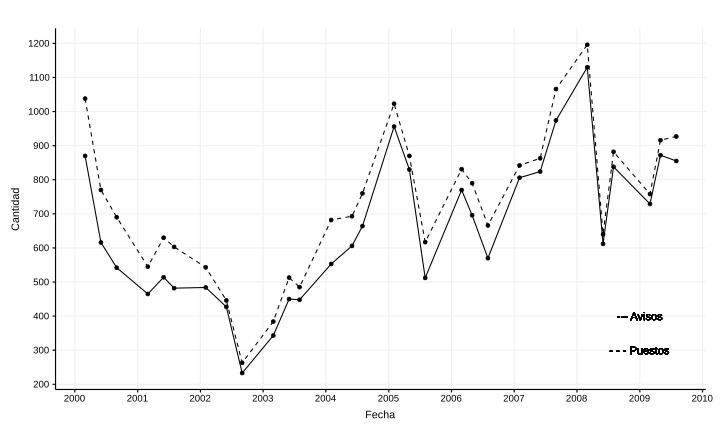
\includegraphics[width=\maxwidth]{tesis_files/figure-latex/iecon-avisos-puestos-1.pdf}
\caption{Serie \textit{Gallito} 2000-2009}\label{fig:iecon-avisos-puestos}\textsc{}

\footnotesize\textsc{Notas} -- Serie de puestos y avisos laborales con frecuencia anual. Serie anual construida en base a los datos de las primeras dos semanas de los meses de marzo, junio y septiembre durante el periodo 2000-2009, construcción propia. Se observa un comovimiento entre avisos y puestos, donde la diferencia es de nivel.

\textsc{Fuentes} -- Datos de Espino et al. (\protect\hyperlink{ref-Alma2011}{2011}), suministrado por autores.
\end{figure}
\newpage

\hypertarget{pea}{%
\subsection{PEA}\label{pea}}
\begin{figure}
\includegraphics[width=\maxwidth]{tesis_files/figure-latex/PeaMontevideo-1.pdf}
\caption{PEA Montevideo 1980-2018}\label{fig:PeaMontevideo}\textsc{}

\footnotesize\textsc{Notas} -- Procesos de fluctuación empíricos bajo el marco de test de fluctuación generalizados. Se visualizan el proceso empírico y su frontera (con color rojo). El proceso supera la frontera indicando la posible existencia de un quiebre estructural en la media incondicional.

\textsc{Fuentes} -- Los datos utilizados son el índice de vacantes de construcción propia y la tasa de desempleo generada por el INE.
\end{figure}

% Index?

\end{document}
